%!TEX TS-program = pdflatex
%!TEX encoding = utf8 
\documentclass[11pt, oneside, openany]{book}
\usepackage[T1]{fontenc}
\usepackage[utf8]{inputenc}
\usepackage[english]{babel}

% ==========================
% = Mathematics & Theorems =
% ==========================
\usepackage{amsmath}
\usepackage{mathtools}
\usepackage{amsthm}
\usepackage{thmtools}

% ===================================================
% = Fonts & Microtypography (NeurIPS / Academic Times) =
% ===================================================
\usepackage{newtxtext}
\usepackage{newtxmath}
\usepackage{bm}
\usepackage{microtype}

% =====================
% = Graphics & Tables =
% =====================
\usepackage{graphicx}
\usepackage{booktabs}
\usepackage{tabularx}
\usepackage{pgfplots}
\pgfplotsset{compat=1.18}
\usepackage{tikz}
\usetikzlibrary{arrows.meta, shadows, positioning, calc, matrix, shapes.geometric, backgrounds, fit}

% ======================================
% = Colors (Sober Academic / NeurIPS)  =
% ======================================
\usepackage{xcolor}
% Deep scholarly navy for links and subtle structure
\definecolor{neuripsblue}{RGB}{14, 38, 92}
\definecolor{darkcharcoal}{RGB}{33, 37, 41}
\definecolor{subtlegray}{RGB}{115, 125, 135}
\definecolor{boxbg}{RGB}{248, 249, 250}
\definecolor{boxborder}{RGB}{210, 215, 222}
% Preserve legacy red as a deep sober burgundy for TikZ diagrams if needed
\definecolor{USred}{RGB}{136, 24, 30}
\definecolor{usred}{RGB}{136, 24, 30}

% =====================
% = Important Data =
% =====================
\title{Mathematical Foundations of Energy-Based Models and Joint Embedding Architectures}
\newcommand{\mysubtitle}[1]{\newcommand{\guardasubtitle}{#1}}
\mysubtitle{From Representation Collapse to World Models}
\author{\large Pedro Rivas Vega}
\date{\today}
\newcommand{\tutores}[1]{\newcommand{\guardatutores}{#1}}
\tutores{Prof. Eduardo S\'anchez Karhunen\\}
\newcommand{\departamento}[2]{\newcommand{\guardadepartamento}{#2}}
\departamento{CCIA}{Computer Science and Artificial Intelligence\\}

% ======================
% = Title Pages =
% ======================
\makeatletter
\edef\maintitle{\@title}
\renewcommand\maketitle{%
  \begin{titlepage}
      \thispagestyle{empty}
      \begin{center}
          \vspace*{0.3cm}
          
          % University seal centered and proportional
          \leavevmode
\includegraphics[height=3.0cm, keepaspectratio]{sello.pdf}\\[0.6cm]
          
          {\scshape\Large Universidad de Sevilla}\\[0.2cm]
          {\scshape\large Facultad de Matem\'aticas}\\[0.15cm]
          {\small\color{subtlegray} Departamento de Ciencias de la Computaci\'on e Inteligencia Artificial}
          
          \vspace{2.0cm}
          
          % Title and Subtitle
          {\LARGE\bfseries\color{neuripsblue} Mathematical Foundations of Energy-Based Models\\[0.25cm] and Joint Embedding Architectures \par}
          \vspace{0.6cm}
          {\large\color{darkcharcoal} \guardasubtitle \par}
          
          \vspace{1.8cm}
          
          % Author
          {\Large\bfseries \@author \par}
          
          \vfill
          
          % Bottom metadata
          \rule{0.6\textwidth}{0.4pt}\\[0.6cm]
          \textbf{\small Supervised by:}\\[0.15cm]
          {\small Prof. Eduardo S\'anchez Karhunen}\\[0.1cm]
          {\small\color{subtlegray} Department of Computer Science and Artificial Intelligence}
          
          \vspace{0.8cm}
          {\small\color{subtlegray} Seville, 2026}
          \vspace*{0.3cm}
      \end{center}
  \end{titlepage}
  
  \pagestyle{tfg}
  \renewcommand{\chaptermark}[1]{\markright{\thechapter.\space ##1}}
  \renewcommand{\sectionmark}[1]{}
  \renewcommand{\subsectionmark}[1]{}
}
\makeatother

% =========================
% = Layout & Typography =
% =========================
\usepackage{enumitem}
\setlist{noitemsep, topsep=3pt}
\usepackage{url}
\usepackage[font=small, labelfont=bf, labelsep=period]{caption}
\usepackage[bottom]{footmisc}
\usepackage{float}

% Highlight boxes (sober academic style)
\usepackage[most]{tcolorbox}
\newtcolorbox{mybox}{
    colback=boxbg,
    colframe=boxborder,
    arc=2pt,
    boxrule=0.6pt,
    fontupper=\small\rmfamily,
    left=10pt, right=10pt, top=7pt, bottom=7pt
}

% ===================================
% = Theorems & Mathematical Styles  =
% ===================================
\declaretheoremstyle[
    spaceabove=7pt plus 2pt minus 1pt,
    spacebelow=7pt plus 2pt minus 1pt,
    headfont=\normalfont\bfseries,
    notefont=\normalfont\bfseries,
    notebraces={(}{)},
    bodyfont=\normalfont\itshape,
    postheadspace=0.6em,
    headindent=0pt,
    headpunct={.}
]{thm_important}

\declaretheoremstyle[
    spaceabove=6pt plus 2pt minus 1pt,
    spacebelow=6pt plus 2pt minus 1pt,
    headfont=\normalfont\bfseries,
    notefont=\normalfont\bfseries,
    notebraces={(}{)},
    bodyfont=\normalfont,
    postheadspace=0.6em,
    headindent=0pt,
    headpunct={.}
]{thm_definition}

\declaretheoremstyle[
    spaceabove=6pt plus 2pt minus 1pt,
    spacebelow=6pt plus 2pt minus 1pt,
    headfont=\normalfont\itshape,
    notefont=\normalfont,
    notebraces={(}{)},
    bodyfont=\normalfont,
    postheadspace=0.6em,
    headindent=0pt,
    headpunct={.},
    numbered=no,
    qed=\qedsymbol
]{thm_proof}

\declaretheorem[name=Theorem, style=thm_important, numberwithin=chapter]{theorem}
\declaretheorem[name=Lemma, style=thm_important, numberwithin=chapter]{lemma}
\declaretheorem[name=Proposition, style=thm_important, numberwithin=chapter]{proposition}
\declaretheorem[name=Corollary, style=thm_important, numberwithin=chapter]{corollary}

\declaretheorem[name=Definition, style=thm_definition, numberwithin=chapter]{definition}
\declaretheorem[name=Remark, style=thm_definition, numberwithin=chapter]{remark}
\declaretheorem[name=Example, style=thm_definition, numberwithin=chapter]{example}

\let\proof=\undefined
\declaretheorem[name=Proof, style=thm_proof]{proof}

% Math Operators
\DeclareMathOperator*{\argmin}{arg\,min}
\DeclareMathOperator*{\argmax}{arg\,max}
\DeclareMathOperator{\Tr}{Tr}
\DeclareMathOperator{\tr}{tr}
\DeclareMathOperator{\rank}{rank}
\DeclareMathOperator{\Ker}{Ker}
\DeclareMathOperator{\Var}{Var}
\DeclareMathOperator{\Cov}{Cov}
\DeclareMathOperator{\diag}{diag}
\DeclareMathOperator{\sg}{sg}
\DeclareMathOperator{\idm}{idm}
\DeclareMathOperator{\SIGReg}{SIGReg}
\DeclareMathOperator{\softmax}{softmax}

% ============================
% = Page Composition =
% ============================
\usepackage[
    a4paper,
    top=3.0cm,
    bottom=3.0cm,
    left=3.2cm,
    right=3.2cm,
    headheight=15pt,
    headsep=15pt,
    footskip=30pt
]{geometry}

\linespread{1.08}
\parskip=4pt plus 1.5pt minus 1pt
\frenchspacing

\setlength{\intextsep}{\bigskipamount}
\setlength{\textfloatsep}{\bigskipamount}

% ========================================
% = Title Formatting (NeurIPS / Academic) =
% ========================================
\usepackage[explicit]{titlesec}

% Chapter formatting: clean, authoritative academic style
\titleformat{\chapter}[hang]
  {\normalfont\LARGE\bfseries\boldmath}
  {\thechapter.\hspace{0.75em}}{0pt}
  {#1}
  [\vspace{0.4ex}\rule{\textwidth}{0.4pt}]

\titleformat{name=\chapter,numberless}[hang]
  {\normalfont\LARGE\bfseries\boldmath}
  {}{0pt}
  {#1}
  [\vspace{0.4ex}\rule{\textwidth}{0.4pt}]

\titlespacing*{\chapter}{0pt}{10pt}{25pt}
\titlespacing*{name=\chapter,numberless}{0pt}{10pt}{25pt}

% Section formatting: NeurIPS style (bold serif, clean hierarchy)
\titleformat{\section}
  {\normalfont\Large\bfseries\boldmath}{\thesection}{0.75em}
  {#1}
\titlespacing*{\section}{0pt}{2.8ex plus 1ex minus .2ex}{1.4ex plus .2ex}

% Subsection formatting
\titleformat{\subsection}
  {\normalfont\large\bfseries\boldmath}{\thesubsection}{0.75em}
  {#1}
\titlespacing*{\subsection}{0pt}{2.2ex plus .8ex minus .2ex}{1.1ex plus .2ex}

% Subsubsection formatting
\titleformat{\subsubsection}
  {\normalfont\normalsize\bfseries\boldmath}{\thesubsubsection}{0.75em}
  {#1}
\titlespacing*{\subsubsection}{0pt}{1.8ex plus .6ex minus .2ex}{0.8ex plus .2ex}

% =======================
% = Page Headers =
% =======================
\usepackage{fancyhdr}
\usepackage{emptypage}
\fancypagestyle{plain}{%
    \fancyhf{}%
    \renewcommand{\headrulewidth}{0pt}
    \renewcommand{\footrulewidth}{0pt}
    \fancyfoot[C]{\small\thepage}
}
\fancypagestyle{tfg}{%
    \fancyhf{}%
    \renewcommand{\headrulewidth}{0.4pt}
    \renewcommand{\footrulewidth}{0pt}
    \fancyhead[LE]{\small\thepage\qquad\textsc{\MakeLowercase{\maintitle}}}
    \fancyhead[RO]{\small\textsc{\MakeLowercase{\rightmark}}\qquad\thepage}%
    \fancyfoot[C]{}%
}

% ============================
% = Hyperlinks & References =
% ============================
\usepackage[
    colorlinks=true,
    linkcolor=neuripsblue,
    citecolor=neuripsblue,
    urlcolor=neuripsblue,
    bookmarksnumbered=true,
    pdfencoding=auto,
    unicode=true
]{hyperref}
\usepackage{cleveref}

% =============================
% = Document starts here =
% =============================
\begin{document}

\maketitle

\frontmatter

\chapter*{Abstract}
\addcontentsline{toc}{chapter}{Abstract}
\markright{Abstract}

Self-Supervised Learning (SSL) has emerged as a cornerstone of modern machine learning, demonstrating that representations of the world can be learned from uncurated data without external human labels. While autoregressive generative models have achieved unprecedented reasoning capabilities in discrete, symbolic domains like natural language, extending these successes to continuous sensory data without the computational burden of pixel-level generative reconstruction requires learning compatibility functions directly in a shared latent space $\mathcal{Z} \subseteq \mathbb{R}^{d}$. This dissertation investigates the mathematical foundations of \textbf{Joint Embedding Architectures} (JEAs) unified under the theoretical framework of \textbf{Energy-Based Models} (EBMs).

The central theoretical challenge articulating this entire work is \textbf{representation collapse}, where encoders minimize energy trivially by mapping observations to a constant or compressing them into a degenerate lower-dimensional subspace. Through spectral and geometric analysis, we trace the formal evolution of anti-collapse mechanisms: (i) Siamese networks, where we prove via gradient flow that positive alignment acts as a contraction operator; (ii) contrastive methods, whose sample complexity scales exponentially as $\mathcal{O}((1/\epsilon)^d)$ due to the metric entropy of the unit sphere $\mathbb{S}^{d-1}$; and (iii) non-contrastive matrix regularizations (Barlow Twins, VICReg), which penalize cross-correlation and covariance but rely on Jaynes' Bridge---a reduction where zero covariance guarantees mutual statistical independence only under an unverified multivariate Gaussian hypothesis. Furthermore, we analyze how temporal extensions (World Models and V-JEPA) attempt to mitigate collapse using empirical heuristics such as Exponential Moving Averages (EMA) and stop-gradient operations that lack a unified statistical foundation.

To resolve these theoretical shortcomings, this thesis examines the mathematical formulation of \textbf{LeWorldModel} and its isotropic probabilistic regularizer, \textbf{SIGReg}. Grounded in the classical \textbf{Cram\'er-Wold Theorem} and the differentiable \textbf{Epps-Pulley test} on the empirical characteristic function, SIGReg projects representations along random one-dimensional directions to actively enforce that $\mathcal{Z} \sim \mathcal{N}(\vec{0}, I_d)$. Because the standard isotropic Gaussian is the maximum entropy distribution under variance constraints, this formulation rigorously guarantees statistical independence, fully closing Barlow's Redundancy Reduction Principle in its original mathematical sense without negative sampling, matrix inversions, or heuristic architectural dynamics.

\vspace{0.8cm}
\noindent\textbf{Keywords:} Self-Supervised Learning, Joint Embedding Architectures, Energy-Based Models, Representation Collapse, Barlow's Principle, Cram\'er-Wold Theorem, Characteristic Function, World Models.

\tableofcontents

\mainmatter

\chapter[Introduction and Foundations of Representation Learning]{Introduction and Foundations of\\ Representation Learning}
\label{chap:1}

If one observes learning as it occurs in nature, in the cognitive development of a child, in the acquisition of language, in the gradual formation of common sense, it becomes reasonable to conjecture that the majority of knowledge is acquired through pure observation of the world, without external labels or rewards. Only a small fraction arises from supervised interaction with a teacher, and an even smaller portion from deliberate trial and error. This hierarchy: observation, supervision, exploration, mirrors Yann LeCun's ``Cake Analogy,'' which placed \textbf{Self-Supervised Learning} (SSL) as the essential substance of any efficient cognitive system. The underlying hypothesis is that, from this process of unsupervised observation, abstract concepts emerge within the network's internal representation space, not as replicas of sensory stimuli, but as abstractions of their invariant relational structure.

This hypothesis has been verified with extraordinary success on natural language. Language constitutes a symbolic proxy for the real world: its domain is discrete, its dimensionality manageable, and the task of predicting the next token implicitly encodes the semantic and logical structure of reality. On this foundation, Large Language Models (LLMs) have demonstrated that SSL at scale produces emergent reasoning capabilities of unprecedented power. The question that opens this thesis is therefore unavoidable: \textit{how can this same reasoning be extended to data far closer to the physical world (vision, video, spatial data, interaction data) which are continuous, high-dimensional, and lack a natural token structure?}

To address it, this thesis explores a paradigm that has lingered since the nineteen-nineties, quiet and parallel to the discriminative and generative approaches that have dominated the history of machine learning: \textbf{Joint Embedding Architectures} (JEAs). Rather than reconstructing the world or classifying it, JEAs learn to project correlated observations into a shared latent space where semantic compatibility replaces superficial similarity. This principle, first articulated in the context of Bromley and LeCun's Siamese networks in 1993, remained at the margins of research for decades. Today, driven by computational scale and theoretical maturity, it stands as one of the most promising building blocks for systems capable of reasoning, predicting the consequences of their actions, and acting autonomously in the physical world. The theoretical framework that unifies them is that of \textbf{Energy-Based Models} (EBMs): unnormalized compatibility functions whose partition function is analytically intractable in the continuous visual domain---in sharp contrast to the discrete, tractable softmax of LLMs---and whose optimal form is grounded, as this thesis demonstrates, in Jaynes' Principle of Maximum Entropy.

The journey this thesis proposes is an \textit{evolutionary one}: from the first Siamese networks and the problem of trivial representation collapse---the central problem articulating the entire work---through contrastive solutions, the non-contrastive matrix regularizations of Barlow Twins and VICReg, the ad-hoc mechanisms of V-JEPA, and finally \textbf{LeWorldModel}: a theoretical synthesis that reduces all anti-collapse regularization to a single scalar functional grounded in the Cram\'er-Wold Theorem and the Epps-Pulley test, rigorously closing Barlow's redundancy reduction circle within predictive architectures. The thesis concludes by looking toward the future with a question the paradigm itself raises---and perhaps with a certain historical vertigo. LeCun's convolutional networks, formulated in the nineteen-eighties, waited nearly four decades for computational scale to vindicate them. Will the JEAs, born in that same era, follow the same trajectory? Are we witnessing, once again, the quiet beginning of the next revolution?

Machine learning has undergone a fundamental transition in its object of study, shifting from optimizing supervised decision boundaries to constructing abstract representations of data. In this chapter, we introduce the foundations of Representation Learning and present the reasons why the JEA paradigm circumvents the formal limitations of traditional generative and discriminative approaches.

\section{Latent Space and Dimensionality Reduction}
\label{sec:1.1}

The central objective of Representation Learning is to construct a parametric model $f_{\theta} \colon \mathcal{X} \to \mathcal{Z}$ that projects data from a high-dimensional observation space $\mathcal{X} \subset \mathbb{R}^{D}$ (where $D$ is the number of pixels, frequencies, or ``raw'' features) into a space $\mathcal{Z} \subseteq \mathbb{R}^{d}$, with $d \ll D$, which we call the \textbf{latent space}, \textbf{embedding space}, or \textbf{representation space}. The key element is that this model is not manually engineered; rather, its parameters $\theta$ are iteratively optimized, generating representations in $\mathcal{Z}$ that encode abstract concepts (e.g., identity, category, or causal relationships) not explicitly present in the raw input data.

\begin{definition}[Latent Space, Encoder, and Embedding Mapping]
\label{def:1.1}
Let $\mathcal{X}$ be the input space and $(\mathcal{Z}, d_{\mathcal{Z}})$ be the latent space, taken as the Euclidean space $\mathbb{R}^{d}$ endowed with the standard Euclidean distance $d_{\mathcal{Z}}(a,b) = \lVert a - b \rVert_{2}$. We define the \textbf{encoder} as a parameterized mapping $f_{\theta} \colon \mathcal{X} \to \mathcal{Z}$, where $\theta \in \Theta$ represents the set of parameters (e.g., weights of a neural network). For each element $x \in \mathcal{X}$, its image $z = f_{\theta}(x) \in \mathcal{Z}$ is called the \textbf{embedding} of $x$.
\end{definition}

Geometrically, we denote by $\mathcal{Z} = f_{\theta}(\mathcal{X})$ the set of all representations generated by the network. This set $\mathcal{Z} \subseteq \mathbb{R}^{d}$ inhabits a $d$-dimensional Euclidean vector space, where $d$ is the number of neurons in the output layer of the encoder (\Cref{app:A}).

\section{Three Paradigms: Discriminative, Generative, and Joint Embedding}
\label{sec:1.2}

Before examining why Joint Embedding Architectures constitute an appropriate foundation for representation learning---and thus for constructing the space $\mathcal{Z}$---it is instructive to analyze the context in which they are framed relative to more traditional approaches.

\subsection{The Discriminative Approach}
\label{sec:1.2.1}

Discriminative models aim to estimate the conditional probability distribution of a target variable or label $y \in \mathcal{Y}$ conditioned on an input datum $x \in \mathcal{X}$:
\begin{equation}
\label{eq:1.1}
p(y \mid x) = \frac{p(x,y)}{p(x)},
\end{equation}
where $p(x,y)$ denotes the joint density of labels and data, and $p(x)$ is the marginal density of the observations. To illustrate this paradigm, consider two typical application scenarios:
\begin{itemize}
    \item \textbf{Image classification:} The input space $\mathcal{X} = [0,1]^{H \times W \times C}$ represents images of dimension $H \times W$ with $C$ color channels, while the label space is discrete and finite, $\mathcal{Y} = \{1, 2, \dots, K\}$, where $K$ represents mutually exclusive categories. The objective is to estimate the probability $p(y = k \mid x)$ for each class $k \in \mathcal{Y}$.
    \item \textbf{Regression (e.g., real estate valuation):} The input space $\mathcal{X} \subset \mathbb{R}^{D}$ encodes $D$ physical and/or historical features of a property (surface area, age, geographic location, number of rooms), while the output space is continuous, $\mathcal{Y} = \mathbb{R}^{+}$, corresponding to its market price. In this case, the model estimates the expected value of the property conditioned on its features, i.e., the conditional expectation $\mathbb{E}[y \mid x]$.
\end{itemize}

Although discriminative modeling forms the pillar of traditional supervised learning \cite{goodfellow2016deep} and is highly effective at solving specific prediction tasks, it exhibits fundamental limitations for learning general data representations \cite{bengio2013representation}. First, its standard supervised formulation relies on a human supervisor to supply labels in $\mathcal{Y}$, a limiting factor in terms of scalability and cost (both computational and human) \cite{lecun2022path}. Second, from an information-theoretic perspective consistent with the Information Bottleneck principle \cite{tishby2000information}, optimizing a model exclusively to predict a target variable forces the gradients to discard all variability and geometric structure of $\mathcal{X}$ that is not strictly useful for solving the task at hand. Discarding features that could prove valuable for secondary or future tasks motivated the search for self-supervised paradigms capable of extracting regularities directly from the intrinsic structure of the data \cite{bengio2013representation}, initially giving way to generative modeling.

\subsection{The Generative Approach}
\label{sec:1.2.2}

The generative approach aims to model the data probability distribution in a way that allows generating or reconstructing samples in the original space $\mathcal{X}$. This paradigm underlies the success of modern foundation models, whether autoregressive architectures (such as GPT) used in natural language processing or diffusion models used for image generation. However, forcing the system to generate or reconstruct the environment can be inefficient.

To reason and ``think'' about the world, it does not seem strictly necessary to recreate it at the pixel level or in full physical detail; operating on abstract representations of its concepts should suffice. Indeed, generative models develop and utilize such abstract representations in their intermediate layers to guide the process. Yet the paradigm forces them to materialize these abstractions into explicit reconstructions in the original space $\mathcal{X}$, introducing severe inefficiencies. For instance, to decide whether it is safe to cross a street, one must predict the future trajectory and behavior of an approaching vehicle; it is inefficient for the model to be forced to concretize that prediction by determining, for example, the exact motion of the background foliage. Generative modeling compels the expenditure of significant computational resources on representing such stochastic details, rather than concentrating solely on the semantic and structural dynamics of the scene in latent space. This inefficiency motivated the search for alternatives that completely bypass physical reconstruction.

\subsection{The Joint Embedding Architectures (JEA) Paradigm}
\label{sec:1.2.3}

The Joint Embedding Architectures paradigm completely bypasses the reconstruction phase. Instead, the system takes two correlated inputs $x, y \in \mathcal{X}$ (e.g., two transformations of the same image, or two consecutive video frames), projects them through two encoders $f_{\theta} \colon \mathcal{X} \to \mathcal{Z}$ and $g_{\phi} \colon \mathcal{X} \to \mathcal{Z}$, and minimizes the distance between their representations in $\mathcal{Z}$:
\begin{equation}
\label{eq:1.2}
\mathcal{L}_{\text{JEA}}(x,y) = \lVert f_{\theta}(x) - g_{\phi}(y) \rVert_{2}^{2},
\end{equation}
where $\theta, \phi \in \Theta$ are the parameters of each encoder, which may be shared ($\theta = \phi$) or independent depending on the specific architecture.

\begin{figure}[H]
\centering
\begin{tikzpicture}[node distance=1.5cm, auto, >=Stealth]
    \node (x) [draw, rectangle, minimum width=2.5cm, minimum height=1cm] {Input $x$};
    \node (y) [draw, rectangle, minimum width=2.5cm, minimum height=1cm, below=of x] {Input $y$};
    \node (fx) [draw, rectangle, minimum width=2cm, minimum height=1cm, right=of x, xshift=1cm] {Encoder $f_{\theta}$};
    \node (gy) [draw, rectangle, minimum width=2cm, minimum height=1cm, right=of y, xshift=1cm] {Encoder $g_{\phi}$};
    \node (zx) [circle, draw, right=of fx, xshift=1cm] {$z_x$};
    \node (zy) [circle, draw, right=of gy, xshift=1cm] {$z_y$};
    \node (loss) [draw, diamond, minimum width=1.5cm, minimum height=1.5cm, right=of zx, yshift=-1.1cm, xshift=1cm] {Loss}; 

    \draw[->] (x) -- (fx);
    \draw[->] (y) -- (gy);
    \draw[->] (fx) -- (zx);
    \draw[->] (gy) -- (zy);
    \draw[->] (zx) -| (loss);
    \draw[->] (zy) -| (loss);
    \draw[dashed, <->] (fx) -- node[left] {Shared $\theta$ (optional)} (gy);
\end{tikzpicture}
\caption{Conceptual diagram of a Joint Embedding Architecture (JEA). The encoders $f_\theta$ and $g_\phi$ project correlated inputs into the latent space $\mathcal{Z}$; the loss penalizes the distance between their representations. Parameter sharing (indicated by the dashed line) is optional and depends on the specific architecture.}
\label{fig:1.1}
\end{figure}

In general, the encoders $f_{\theta}$ and $g_{\phi}$ may have different parameters. However, in most practical implementations, both encoders share the same weights ($\theta = \phi$). This guarantees that the projection function is identical for both branches, so that identical inputs necessarily produce the same embedding.

By not requiring a decoder operating in $\mathbb{R}^{D}$, JEAs do not invest model capacity in task-irrelevant details such as those discussed earlier. The encoder acts as a filter that retains only semantically relevant information, structuring the space $\mathcal{Z}$ so that geometric similarity reflects semantic similarity.

Nevertheless, this paradigm raises critical questions. First, does the optimization process guarantee that the obtained representation faithfully recovers the true degrees of freedom of the physical world (the generating latent variables), or does it risk distorting them so that they lose their structure? This is the problem of \textbf{representation collapse} \cite{jing2022understanding}. Second, is it possible to optimally plan and control an agent within this space without degrading its real-world performance? \Cref{chap:6} introduces the temporal dimension by incorporating a planning window within these latent spaces and analyzes the JEPA-style solutions developed to avoid collapse. Subsequently, \Cref{chap:7} explores the isotropic regularization solution (SIGReg) proposed in 2025 \cite{balestriero2025lejepa} as an evolution overcoming VICReg-style matrix methods, paving the way toward planning in the space $\mathcal{Z}$.

In this thesis, we address the historical and conceptual trajectory that has consolidated the Joint Embedding Architectures paradigm. The guiding thread is the resolution of the paradigm's most persistent obstacle: \textit{representation collapse}, wherein the network minimizes energy to zero by mapping all inputs to a trivial constant $f_{\theta}(x) = c$. The central notion is that of \textbf{compatibility}: an unnormalized measure quantifying the degree of semantic correspondence between two input variables, whose formalization via energy functions is developed in the next chapter, where Energy-Based Models (EBMs) are formally introduced as a unifying framework for compatibility learning, comparing discrete and continuous scenarios and laying the physical foundations of Jaynes' Principle of Maximum Entropy.

% =========================================================================
% CHAPTER 2
% =========================================================================
\chapter{Energy-Based Models and Compatibility Learning}
\label{chap:2}

\section{Introduction to Energy-Based Models and the Energy Landscape}
\label{sec:2.1}

Energy-Based Models (EBMs) provide a flexible mathematical framework for designing artificial intelligence systems \cite{lecun2006tutorial}. In the context of this work, they constitute the formal foundation of Joint Embedding Architectures (JEAs). Unlike probabilistic models, which require strict normalization, EBMs evaluate the compatibility between variables by assigning them an unnormalized scalar termed ``energy.'' Intuitively, low energy indicates that the combination of variables is highly plausible or compatible, whereas high energy denotes incompatibility. This metric can be visualized as an ``energy landscape'' where valleys (local minima) represent configurations of interest, and peaks (energy maxima) represent ``implausible'' configurations or noise. If the model fails and maps every combination to the same energy (for instance, zero), the energy landscape flattens completely. This destructive phenomenon is known as \textbf{representation collapse}.

\subsection{The Energy Function and Its Probabilistic Independence}
\label{sec:2.1.1}

In prediction and representation learning tasks (such as JEAs), the model operates on the joint space of configurations, defined as the product space $\mathcal{C} = \mathcal{X} \times \mathcal{Y}$, where $x \in \mathcal{X}$ represents the observed variable or system input (e.g., image context or video frame) and $y \in \mathcal{Y}$ is the prediction or target variable to be evaluated. The centerpiece of the model is the conditional energy function:
\begin{equation}
\label{eq:2.1}
E_{\theta}(x,y) \in \mathbb{R},
\end{equation}
where $\theta$ denotes the trainable parameters of the model (neural network weights). The scalar $E_{\theta}(x,y)$ directly measures the discrepancy between $x$ and $y$. This energy is characterized by its complete independence from Kolmogorov's axioms:
\begin{itemize}
    \item \textbf{Non-negativity:} Unlike probability densities, $E_{\theta}(x,y)$ can take negative real values.
    \item \textbf{Normalization:} It does not require the integral over the prediction space to sum to unity: $\int_{\mathcal{Y}} E_{\theta}(x,y')\,dy' \neq 1$.
\end{itemize}

This flexibility allows JEAs to focus exclusively on the energy surface, avoiding the computation of complex normalization constants and channeling model capacity into the semantic dynamics of the data within their representations.

\subsection{Inference in Energy-Based Models}
\label{sec:2.1.2}

Performing inference in an EBM consists of searching for the state $y$ that minimizes the energy for a given observed input $x$. Unlike the probabilistic approach, which computes expectations or integrals over the entire output space, unnormalized inference reduces to an optimization or global minimum search problem:
\begin{equation}
\label{eq:2.2}
y^{*} = \argmin_{y \in \mathcal{Y}} E_{\theta}(x,y).
\end{equation}

In \Cref{fig:2.1}, this idea is illustrated for image classification. Given an observed input $x$ (an image of a dog), the model evaluates the energy $E_{\theta}(x,y)$ for each candidate class $y$. The inferred response is the class that produces the minimum energy value (represented by the shortest bar).

\begin{figure}[H]
    \centering
    \begin{tikzpicture}[
        >=stealth,
        textfont/.style={font=\small\sffamily, align=center},
        labelsbox/.style={draw, align=left, inner sep=1.5ex, font=\small\sffamily, text depth=0pt}
    ]
        \node (img) {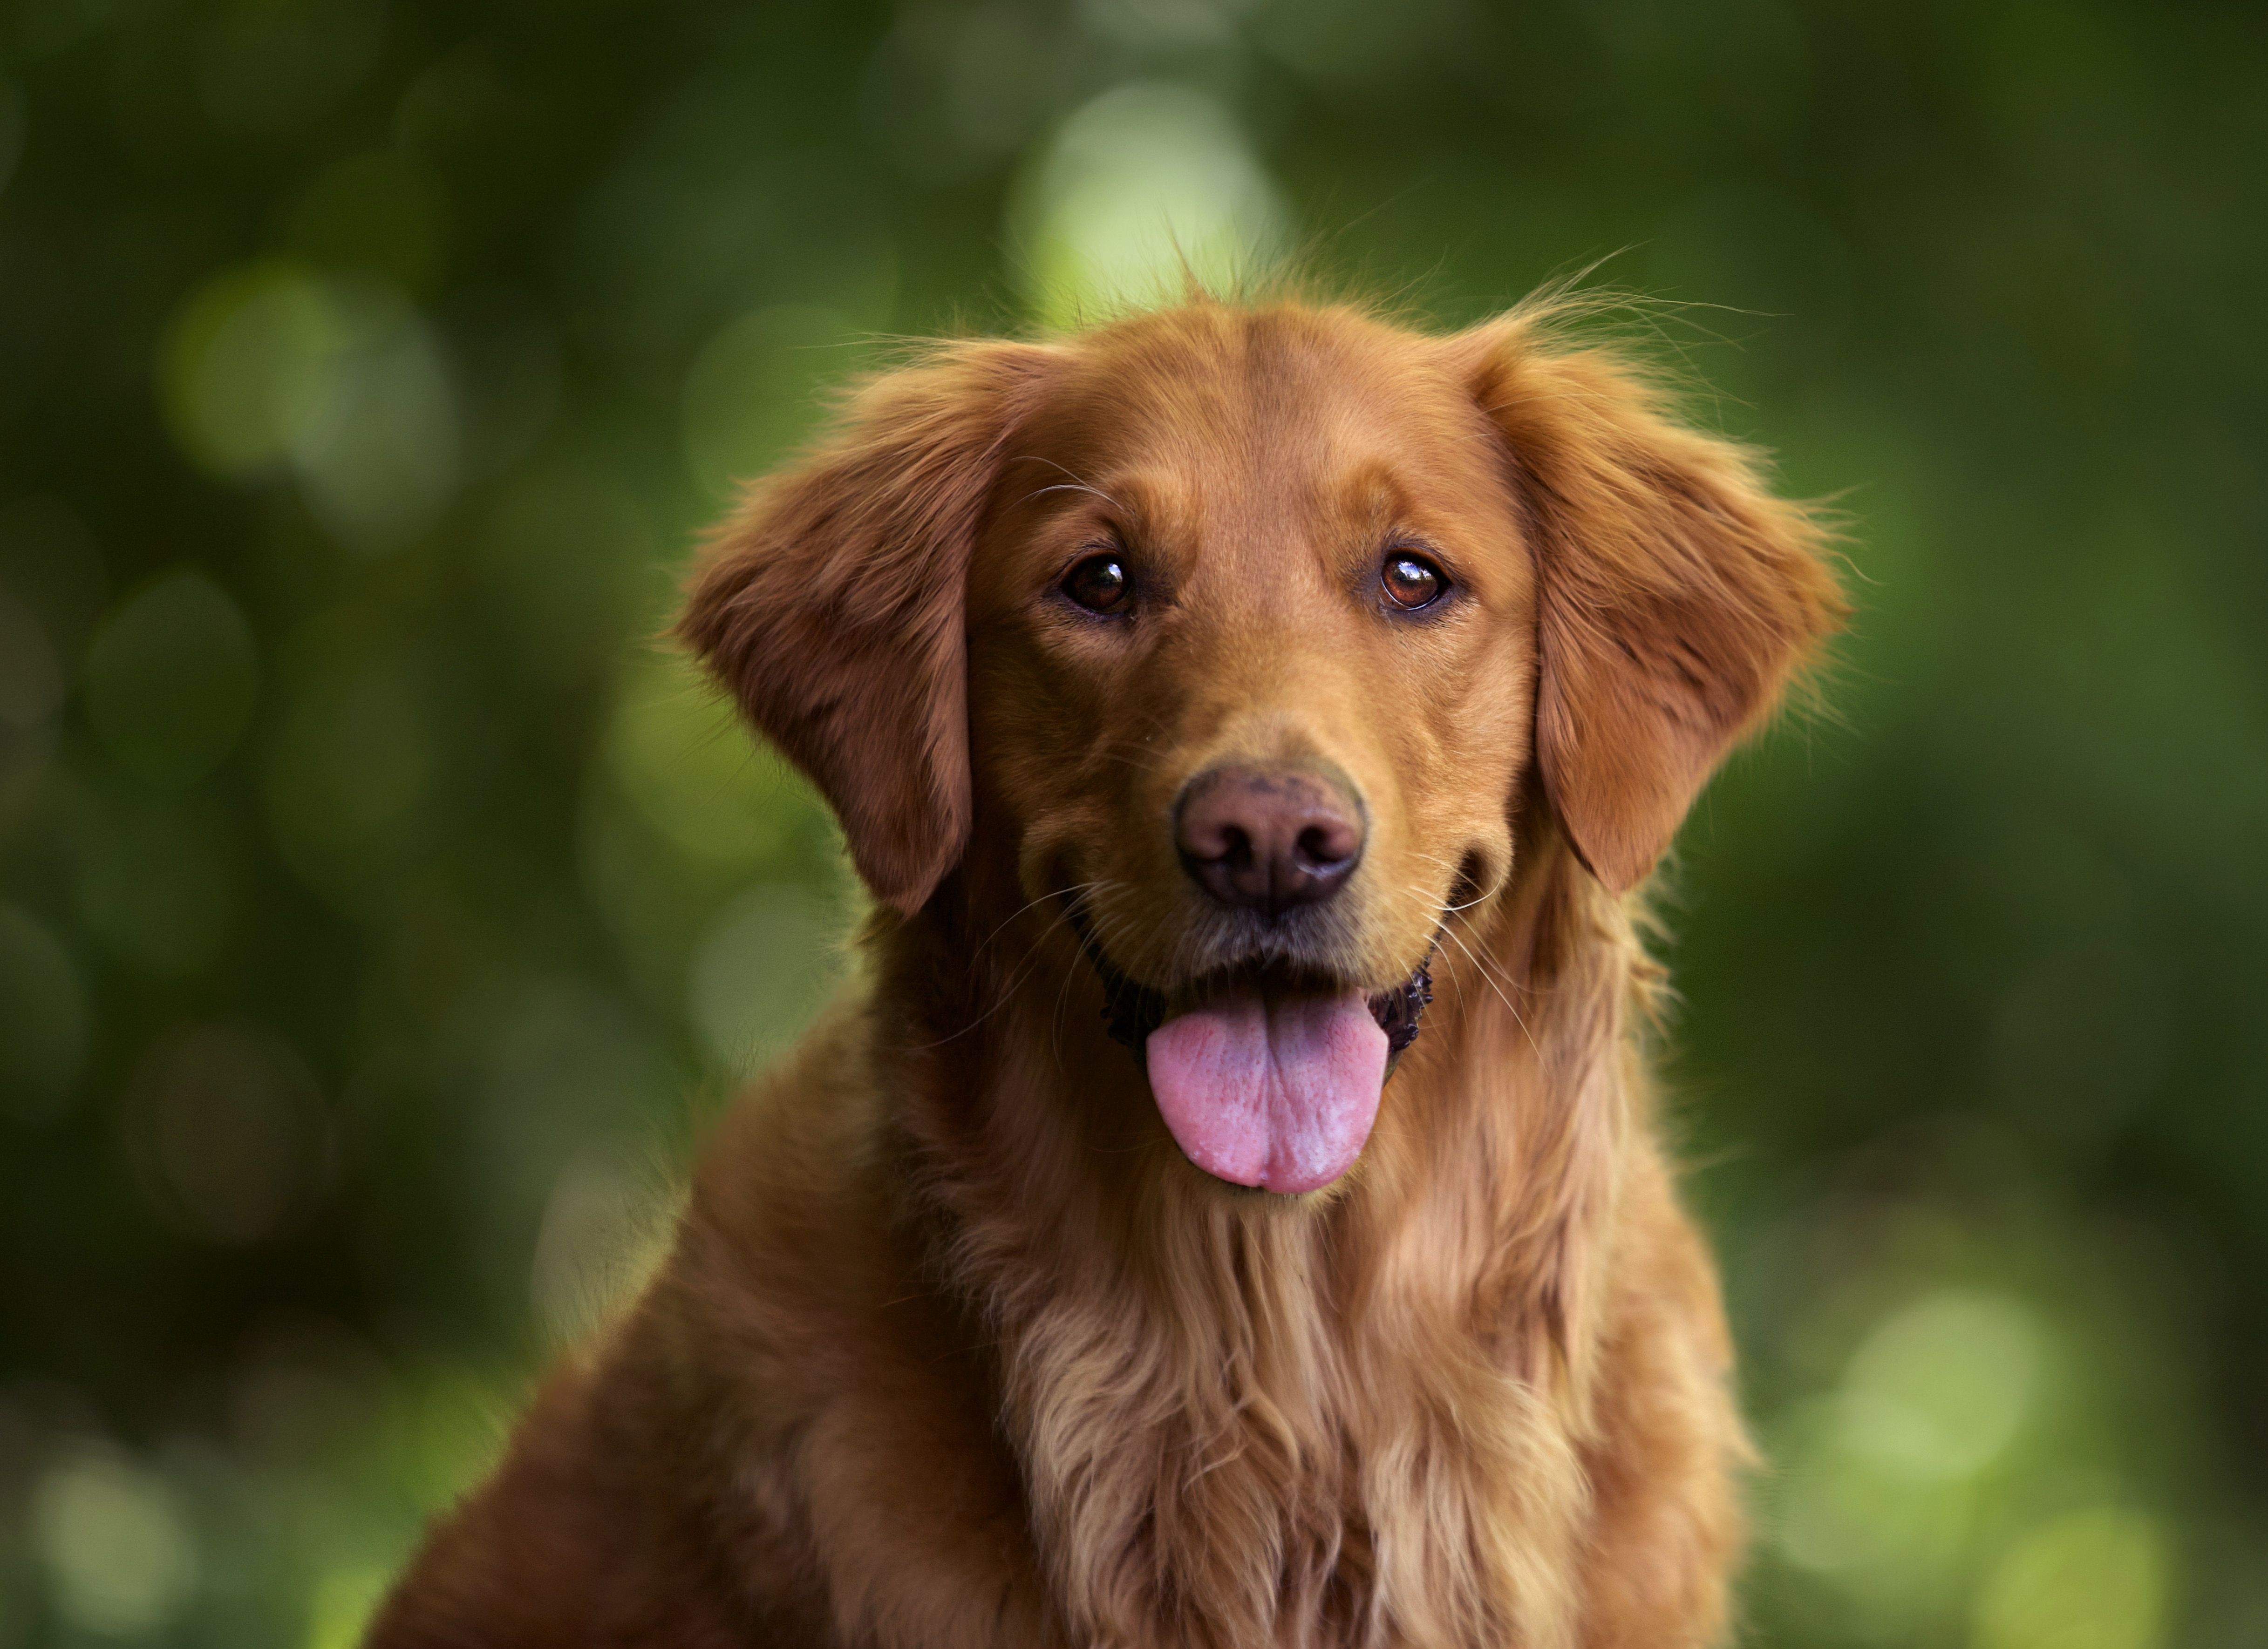
\includegraphics[width=1.6cm]{selective-focus-shot-adorable-golden-retriever-outdoors.jpg}};
        \node[above=0.15cm of img, textfont] (x_text) {$x$\\Observed input};

        \node[right=1.8cm of img, labelsbox] (y_box) {
            Human \\ Animal \\ Airplane \\ Car \\ Truck
        };
        \node[above=0.15cm of y_box, textfont] (y_text) {$y$\\Candidate class};

        \node[draw, rounded corners, minimum width=6.2cm, minimum height=0.9cm,
              above=0.9cm of $(x_text.north)!0.5!(y_text.north)$,
              font=\small\sffamily] (ef) {Energy Function\quad $E_\theta(x, y)$};

        \draw[->, thick] (x_text) -- (x_text |- ef.south);
        \draw[->, thick] (y_text) -- (y_text |- ef.south);
        \draw[->, thick] (ef.north) -- ++(0, 0.8cm) coordinate (out_arrow);

        \begin{scope}[shift={($(ef.north)+(0, 0.9cm)$)}]
            \tikzset{bar/.style={draw, fill=gray!70, minimum height=0.18cm,
                     inner sep=0pt, anchor=west}}
            \node[left, font=\scriptsize\sffamily] at (0, 1.0) {Human};
            \node[bar, minimum width=1.3cm] at (0.1, 1.0) {};
            \node[left, font=\scriptsize\sffamily] at (0, 0.75) {\textbf{Animal}};
            \node[bar, minimum width=0.25cm] at (0.1, 0.75) {};
            \node[left, font=\scriptsize\sffamily] at (0, 0.5) {Airplane};
            \node[bar, minimum width=1.6cm] at (0.1, 0.5) {};
            \node[left, font=\scriptsize\sffamily] at (0, 0.25) {Car};
            \node[bar, minimum width=1.0cm] at (0.1, 0.25) {};
            \node[left, font=\scriptsize\sffamily] at (0, 0.0) {Truck};
            \node[bar, minimum width=0.8cm] at (0.1, 0.0) {};
            \draw[->, thick] (0.1, -0.15) -- (2.0, -0.15);
            \node[below, font=\scriptsize\sffamily] at (1.05, -0.15) {$E_\theta(x, y)$};
        \end{scope}
    \end{tikzpicture}
    \caption{Energy in the context of EBMs for a classification task. Given the observed input $x$ (image of a dog), the model evaluates the energy $E_\theta(x, y)$ for each candidate class $y$. The inferred answer is $y = \text{Animal}$, as it has the minimum associated energy value among candidate classes (shortest bar). Notice that it requires no probabilistic normalization.}
    \label{fig:2.1}
\end{figure}

\section{The Boltzmann-Gibbs Measure and Inverse Temperature}
\label{sec:2.2}

To perform probabilistic inference or train EBMs via maximum likelihood, it is necessary to transform the energy function $E_{\theta}(x,y)$ into a conditional probability distribution $p_{\theta}(y \mid x)$ over the prediction space $\mathcal{Y}$. This correspondence is established through the conditional Boltzmann-Gibbs measure:
\begin{equation}
\label{eq:2.3}
p_{\theta}(y \mid x) = \frac{\exp(-\beta E_{\theta}(x,y))}{Z(x;\theta)},
\end{equation}
where $\beta > 0$ is the inverse temperature (or selection intensity, $\beta = 1/T$) controlling the dispersion of the landscape, and $Z(x;\theta)$ is the conditional partition function normalizing the measure (if $\mathcal{Y}$ is discrete, the integral becomes a summation):
\begin{equation}
\label{eq:2.4}
Z(x;\theta) = \int_{\mathcal{Y}} \exp(-\beta E_{\theta}(x,y'))\,dy'.
\end{equation}

The temperature parameter $\beta$ directly modulates probabilistic concentration in the valleys of the energy landscape. As illustrated in \Cref{fig:2.2}, a low value of $\beta$ (high temperature) smooths the distribution, making it more uniform, whereas a high value of $\beta$ (low temperature) strongly concentrates the conditional probability mass in the global energy minima of $\mathcal{Y}$.

\begin{figure}[htbp]
    \centering
    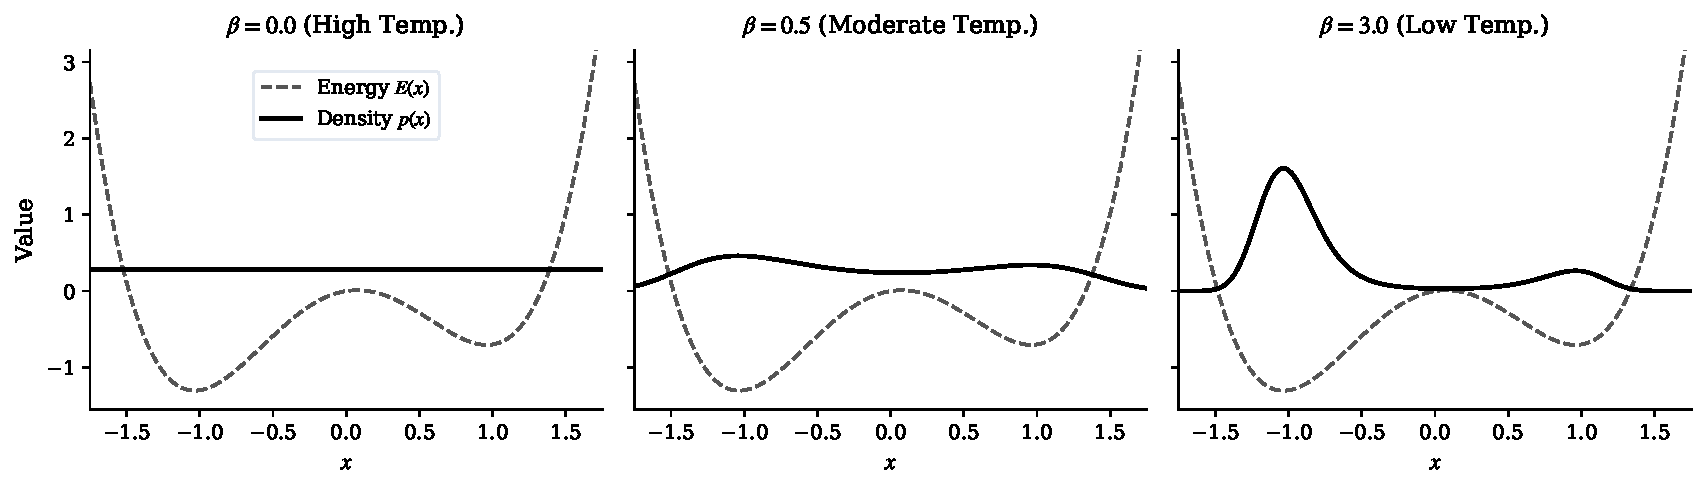
\includegraphics[width=0.95\textwidth]{beta_temperature.pdf}
    \caption{Evolution of the Boltzmann-Gibbs density associated with the example energy function $E(x) = x^4 - 2x^2 + 0.3x$, for different values of $\beta$. Left: $\beta = 0.0$ (high temperature), uniform distribution. Center: $\beta = 0.5$ (medium temperature), smooth bimodality; probability mass transitions easily between valleys. Right: $\beta = 3.0$ (low temperature), probability mass strongly concentrates in the global energy minimum.}
    \label{fig:2.2}
\end{figure}

\section{Jaynes' Principle of Maximum Entropy}
\label{sec:2.3}

The choice of the conditional Boltzmann-Gibbs distribution in \Cref{eq:2.3} can be grounded in information-theoretic principles. It is the unique probability distribution that maximizes conditional entropy subject to first-moment constraints on the energy.

Jaynes' Principle of Maximum Entropy \cite{jaynes1957information} states that, for a fixed input $x \in \mathcal{X}$, the conditional probability distribution $p(y \mid x)$ that best represents our state of knowledge about the target variable $y$ is the one that maximizes Shannon's conditional entropy:
\begin{equation}
\label{eq:2.5}
\max_{p(\cdot \mid x)} H(p(y \mid x)) = -\sum_{y \in \mathcal{Y}} p(y \mid x) \log p(y \mid x),
\end{equation}
subject to the physical constraints imposed by the observations:
\begin{align}
\text{Normalization:} \quad & \sum_{y \in \mathcal{Y}} p(y \mid x) = 1, \label{eq:2.6} \\
\text{Energy moments:} \quad & \sum_{y \in \mathcal{Y}} p(y \mid x) f_{k}(x,y) = \mu_{k}(x), \quad \forall k = 1, \dots, K, \label{eq:2.7}
\end{align}
where $f_{k}(x,y)$ are feature functions and $\mu_{k}(x)$ are their known expected values.

Analytical resolution of this optimization problem via conditional Lagrange multipliers $\lambda_{k}(x)$ uniquely determines the maximum entropy conditional distribution as:
\begin{equation}
\label{eq:2.8}
p(y \mid x) = \frac{1}{Z(x)} \exp\left(-\sum_{k=1}^{K} \lambda_{k}(x) f_{k}(x,y)\right),
\end{equation}
with partition function $Z(x) = \sum_{y' \in \mathcal{Y}} \exp\left(-\sum_{k=1}^{K} \lambda_{k}(x) f_{k}(x,y')\right)$. This form coincides with the conditional Boltzmann-Gibbs distribution, where the multipliers $\lambda_{k}(x)$ play the role of the conditional inverse temperature $\beta$.

\subsection{Adaptive Connection with Deep Neural Networks}
\label{sec:2.3.1}

Jaynes' formulation uses a linear combination of physical features $f_{k}(x,y)$ chosen \textit{a priori}:
\begin{equation}
\label{eq:2.9}
E_{\text{Jaynes}}(x,y) = \sum_{k=1}^{K} \lambda_{k}(x) f_{k}(x,y).
\end{equation}
In Representation Learning, manually defining these joint features for complex data is impracticable. Deep Neural Networks resolve this limitation by replacing fixed functions $f_{k}(x,y)$ with adaptive representations learned from data.

As detailed in \Cref{app:A}, a deep neural network processes the joint input $(x,y)$ through its nonlinear hidden layers to compute the energy. The scalar output of the energy functional $E_{\theta}(x,y)$ can be interpreted at its output layer as a linear combination of the features from the last hidden layer, $\phi_{k}(x,y;\theta_{\text{feat}})$, weighted by weights $w_{k}$ and a bias $b$:
\begin{equation}
\label{eq:2.10}
E_{\theta}(x,y) = \sum_{k=1}^{d} w_{k} \phi_{k}(x,y;\theta_{\text{feat}}) + b,
\end{equation}
where $\theta = (\theta_{\text{feat}}, w, b)$ represents all network parameters. The neural network not only optimizes the multipliers $\lambda_{k}(x) = w_{k}$, but adaptively learns the features $f_{k}(x,y) = \phi_{k}(x,y)$ themselves via backpropagation.

\subsection{The Probabilistic Dilemma and the Leap to Geometry}
\label{sec:2.3.2}

Jaynes' thermodynamic formulation provides the ideal probability distribution representing our knowledge (Maximum Conditional Entropy). However, as detailed in the next section, the computational bottleneck of the partition integral in high-dimensional continuous spaces forces us to abandon this ``thermodynamic perfection.''

By dispensing with the normalization $Z$ and the ``probabilistic wrapper'' $p_{\theta}(y \mid x)$, the model is left with an energy surface that is not probabilistically bounded. Energy comes to be interpreted purely geometrically, with the network directly computing a value $E_{\theta}(x,y)$. This abandonment of probability explains why in subsequent chapters (addressing practical implementations of these systems) the language of probabilities disappears almost entirely in favor of linear algebra, variance, and spatial Euclidean distance.

\section{The Probabilistic Bottleneck: Intractability of $Z(x;\theta)$}
\label{sec:2.4}

Although the conditional Boltzmann-Gibbs measure elegantly formalizes the conditional probability $p_{\theta}(y \mid x)$ from the energy $E_{\theta}(x,y)$, the conditional partition function $Z(x;\theta)$ represents a severe computational bottleneck in high-dimensional continuous spaces.

\subsection{Discrete vs. Continuous Scenario}
\label{sec:2.4.1}

In finite discrete spaces $\mathcal{Y} = \{y_{1}, \dots, y_{K}\}$ (such as the vocabulary of an LLM), the partition function reduces to a finite sum:
\begin{equation}
\label{eq:2.11}
Z(x;\theta) = \sum_{k=1}^{K} e^{-\beta E_{\theta}(x,y_{k})}.
\end{equation}
Applying normalization over this sum yields the Softmax operator, which is tractable in discrete domains. Conversely, in continuous domains such as images or videos $\mathcal{Y} \subseteq \mathbb{R}^{D}$, the dimension of the space (the number of pixels or continuous variables) can easily reach the order of $D \approx 10^{6}$. It is crucial to distinguish this dimensionality from the total number of possible configurations: even if we discretized each variable into just 256 intensity levels, the cardinality of the search space would be $256^{D} \approx 10^{2.4 \times 10^{6}}$ combinations---a value exceeding by orders of magnitude the number of atoms in the observable universe (traditionally estimated at $\sim 10^{80}$). In the continuous case, the partition function is given by the Lebesgue integral:
\begin{equation}
\label{eq:2.12}
Z(x;\theta) = \int_{\mathcal{Y}} e^{-\beta E_{\theta}(x,y')}\,dy'.
\end{equation}
This integral lacks an analytical solution for nonlinear energy functions modeled by neural networks. Furthermore, any direct numerical approximation (such as quadrature) is infeasible due to the \textit{curse of dimensionality}, as the number of evaluation points grows exponentially with $D$.

\subsection{The Log-Partition Gradient and MCMC}
\label{sec:2.4.2}

When working with likelihood functions, the intractability of the normalization term $Z(x;\theta)$ propagates to the computation of the log-likelihood gradient. Since neural network training relies on gradient descent (\Cref{sec:A.3}), this intractability obstructs the optimization process. The gradient of the log-partition function with respect to the parameters $\theta$ is obtained as:
\begin{align}
\nabla_{\theta} \log Z(x;\theta) &= \frac{1}{Z(x;\theta)} \nabla_{\theta} \int_{\mathcal{Y}} e^{-\beta E_{\theta}(x,y')}\,dy' \nonumber \\
&= -\beta \int_{\mathcal{Y}} \frac{e^{-\beta E_{\theta}(x,y')}}{Z(x;\theta)} \nabla_{\theta} E_{\theta}(x,y')\,dy' \nonumber \\
&= -\beta \mathbb{E}_{p_{\theta}(y \mid x)}[\nabla_{\theta} E_{\theta}(x,y)]. \label{eq:2.13}
\end{align}

Evaluating this gradient requires computing the mathematical expectation under the model's own distribution $p_{\theta}(y \mid x)$. Because we cannot evaluate $Z(x;\theta)$, we cannot sample from $p_{\theta}$ directly and must resort to Markov Chain Monte Carlo (MCMC) algorithms, such as Langevin dynamics. In realistic pixel-dimension scenarios, MCMC is prohibitive due to:
\begin{itemize}
    \item \textbf{Slow convergence:} It requires executing hundreds of neural network inference steps for each individual sample during the optimization loop.
    \item \textbf{Mode mixing:} The conditional density of real images is highly multimodal. MCMC chains become trapped in local energy minima and fail to transition between distant modes, biasing the gradient estimator.
\end{itemize}

This barrier motivates abandoning the probabilistic paradigm: JEAs dispense entirely with probabilistic normalization and $Z(x;\theta)$, operating in an unnormalized manner within the latent space.

\section{EBMs as a Framework for Compatibility Learning (SSL)}
\label{sec:2.5}

In Self-Supervised Learning (SSL), the objective is not to classify or predict external labels, but to capture the intrinsic structure of data from consistency relations. In this context, EBMs are formulated over the joint space $\mathcal{X} \times \mathcal{Y}$ to evaluate mutual compatibility of variables via the energy function $E_{\theta}(x,y)$. A low energy value $E_{\theta}(x,y)$ indicates that the pair of variables is consistent or compatible, whereas a high value represents incompatibility. This compatibility framework adapts naturally to SSL \textit{pretext tasks} (auxiliary tasks designed to extract supervisory signals from the data themselves):
\begin{enumerate}
    \item \textbf{Masked region prediction (Inpainting):} Let $x_{o} \in \mathcal{X}_{o}$ be the observed portion of an image and $x_{h} \in \mathcal{X}_{h}$ the hidden region to be predicted. The EBM learns an energy function $E_{\theta}(x_{o}, x_{h})$ that takes minimum values only when $x_{h}$ is a visually coherent continuation of $x_{o}$.

\begin{figure}[htbp]
    \centering
    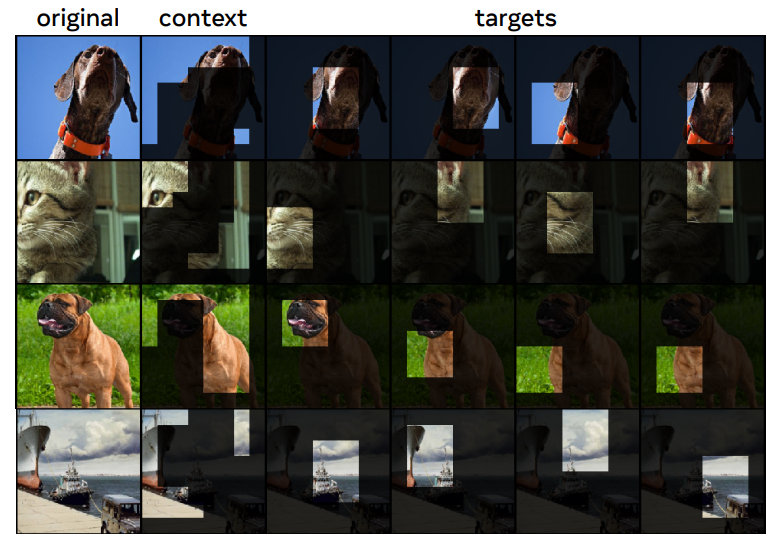
\includegraphics[width=0.8\textwidth]{SSL_inpainting.png}
    \caption{Representation of masked region prediction (Inpainting). The observed portion $x_o$ (context) and the true hidden portion $x_h$ (target) form a low-energy pair $E_\theta(x_o, x_h)$, while incorrect patches raise the energy.}
    \label{fig:2.3}
\end{figure}

    \item \textbf{Consistency across augmented views:} Given two augmented transformations of the same sample $x$, denoted $x_{1} = T_{1}(x)$ and $x_{2} = T_{2}(x)$, the model evaluates their compatibility via $E_{\theta}(x_{1}, x_{2})$. The EBM is optimized to assign low energies to views originating from the same source sample and high energies to views from distinct samples.
\end{enumerate}

\subsection{Compatibility Modeling Without Probability Densities}
\label{sec:2.5.1}

The success of EBMs in SSL lies in modeling compatibility directly via the unnormalized energy function $E_{\theta}(x,y)$, avoiding the estimation of normalized conditional densities $p_{\theta}(y \mid x)$. By dispensing with normalization, one completely circumvents the intractability of computing the conditional partition function $Z(x;\theta)$ in high-dimensional continuous spaces such as pixels (\Cref{sec:2.4}).

\subsection{JEAs as Non-Probabilistic EBMs}
\label{sec:2.5.2}

The Joint Embedding Architectures (JEA) paradigm is a concrete realization of non-probabilistic EBMs in latent space. Rather than evaluating input compatibility in the physical pixel space $\mathbb{R}^{D}$, JEAs project $x$ and $y$ into a low-dimensional latent space $\mathcal{Z} \subseteq \mathbb{R}^{d}$ ($d \ll D$) using two encoders $f_{\theta}$ and $g_{\phi}$.

The energy function of the JEA is defined as the squared Euclidean distance between the latent embeddings of both variables:
\begin{equation}
\label{eq:2.14}
E_{\theta,\phi}(x,y) = \mathcal{L}_{\text{JEA}}(x,y) = \lVert f_{\theta}(x) - g_{\phi}(y) \rVert_{2}^{2}.
\end{equation}

This formulation provides three crucial advantages:
\begin{enumerate}
    \item \textbf{Reconstruction is avoided:} Compatibility is measured directly in $\mathcal{Z}$. The encoders act as information filters that discard high-frequency stochastic noise (such as background details) and retain only robust semantic features.
    \item \textbf{Absence of normalization:} \Cref{eq:2.14} is strictly unnormalized. It avoids computing the conditional partition function $Z(x;\theta)$ over continuous images, resolving the predictive bottleneck of the Lebesgue integral in $\mathbb{R}^{D}$.
    \item \textbf{Semantic geometrization:} The energy surface is defined by the metric of $\mathcal{Z}$. Minimizing energy brings latent representations of coherent samples closer together, structuring the geometry of the embedding space.
\end{enumerate}

As detailed in \Cref{chap:3}, the major limitation of this non-probabilistic approach is that, lacking conditional normalization or negative samples, the system naturally tends toward \textbf{representation collapse}: a degenerate solution where the encoders become constant ($f_{\theta}(x) = g_{\phi}(y) = c$), trivially minimizing energy to zero without extracting any semantic information from reality.

% =========================================================================
% CHAPTER 3
% =========================================================================
\chapter{Origins of Joint Embedding: Siamese Networks and Representation Collapse}
\label{chap:3}

The idea of comparing representations rather than reconstructing physical inputs dates back to the early 1990s with the introduction of Siamese networks. However, this paradigm soon encountered a fundamental obstacle: \textbf{Representation Collapse}. In this chapter, we formally analyze Siamese networks and mathematically derive the causes of this collapse.

\section{Bromley's Siamese Networks (1993)}
\label{sec:3.1}

Siamese networks were conceived by Jane Bromley and Yann LeCun at Bell Labs \cite{bromley1993signature} to solve the practical problem of handwritten signature verification. The central idea is to construct an encoder that projects data belonging to the same person (same semantic class) to nearby points in the embedding space $\mathcal{Z}$, and signatures from different people (or forged signatures) to distant points.

\begin{definition}[Siamese Network Architecture]
\label{def:3.1}
Let $\mathcal{X} \subseteq \mathbb{R}^{D}$ be the input image space. Consider a single neural network model parameterized by a weight vector $W \in \mathbb{R}^{M}$, defining a differentiable function $f_{W} \colon \mathbb{R}^{D} \to \mathbb{R}^{d}$. The Siamese architecture consists of two identical copies of this function (sharing the exact same parameter vector $W$). Given two inputs $x_{1}, x_{2} \in \mathcal{X}$, the network computes their embeddings in parallel:
\begin{equation}
\label{eq:3.1}
z_{1} = f_{W}(x_{1}), \qquad z_{2} = f_{W}(x_{2}).
\end{equation}
The distance metric in the latent space is defined via the Euclidean distance:
\begin{equation}
\label{eq:3.2}
d_{W}(x_{1}, x_{2}) = \lVert f_{W}(x_{1}) - f_{W}(x_{2}) \rVert_{2}.
\end{equation}
\end{definition}

Although the Euclidean distance $d_{W}$ measures geometric dissimilarity, the loss formulation typically employs its square, known as the mean squared error, to guarantee gradient differentiability at the origin (quadratic distance, \Cref{sec:A.2} of \Cref{app:A}). This shared-weight structure ensures that two identical inputs $x_{1} = x_{2}$ are necessarily projected to the exact same point in $\mathcal{Z}$, $z_{1} = z_{2}$, preserving the reflexivity of the distance.

\section{Representation Collapse}
\label{sec:3.2}

Representation collapse occurs when the network finds a trivial solution that minimizes the distance $d_{W}$ between similar samples without extracting useful features from the data.

\begin{remark}[Population Notation]
\label{rem:3.1}
This section adopts a theoretical approach; therefore, empirical estimators over minibatches will often be replaced by their population counterparts---for instance, the sample average will be replaced by the mathematical expectation ($\mathbb{E}$) over the true data distribution ($p_{\text{pos}}$ and $p_{\text{data}}$). Although practical training is performed on finite sets, this approach allows a more rigorous analysis of the causes of collapse by eliminating the noise and limitations of empirical sampling.
\end{remark}

\subsection{Constant Collapse as a Global Minimum}
\label{sec:3.2.1}

Consider a training scenario where we only have access to an empirical set of compatible pairs (also called positive pairs) $\mathcal{D} = \{(x_{1}^{(i)}, x_{2}^{(i)})\}_{i=1}^{N}$. These pairs represent compatible instances, such as multiple views of the same object or, in the original Siamese networks, two signatures from the same person. In practice, the network's objective is to minimize the average of the squared distances over this set or over minibatches (\Cref{sec:A.2.3}):
\begin{equation}
\label{eq:3.3}
\hat{\mathcal{L}}_{\text{pos}}(W) = \frac{1}{N} \sum_{i=1}^{N} \lVert f_{W}(x_{1}^{(i)}) - f_{W}(x_{2}^{(i)}) \rVert_{2}^{2}.
\end{equation}

However, assuming the pairs are drawn from a joint distribution $p_{\text{pos}}(x_{1}, x_{2})$ over $\mathcal{X} \times \mathcal{X}$, the true purpose is to optimize the model over the entire underlying data population. Consequently, theoretical analysis requires abstracting away from the empirical sum and defining the global loss function as the mathematical expectation of the squared distance:
\begin{equation}
\label{eq:3.4}
\mathcal{L}_{\text{pos}}(W) = \mathbb{E}_{(x_{1}, x_{2}) \sim p_{\text{pos}}} \left[ \lVert f_{W}(x_{1}) - f_{W}(x_{2}) \rVert_{2}^{2} \right].
\end{equation}

This expectation-based formulation is the standard adopted in the literature \cite{wang2020understanding}. From this population objective, we can prove that constant collapse is both a global minimum and a stable attractor of the gradient for this loss function.

\begin{figure}[H]
\centering
\begin{tikzpicture}[node distance=1.5cm, auto, >=Stealth]
    \node (x1) [draw, rectangle, minimum width=2.5cm, minimum height=1.5cm] {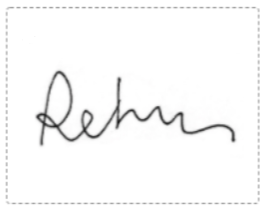
\includegraphics[width=2.3cm, height=1.3cm]{signature_Rodlf1.png}};
    \node (x2) [draw, rectangle, minimum width=2.5cm, minimum height=1.5cm, below=of x1, yshift=-0.5cm] {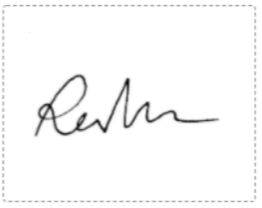
\includegraphics[width=2.3cm, height=1.3cm]{signature_Rodlf2.png}};
    
    \node [above=0.05cm of x1, font=\footnotesize] {Input $x_1$ (Signature A)};
    \node [below=0.05cm of x2, font=\footnotesize] {Input $x_2$ (Signature B)};
    
    \node (f1) [draw, rectangle, minimum width=2cm, minimum height=1cm, right=of x1, xshift=1cm] {Encoder $f_{W}$};
    \node (f2) [draw, rectangle, minimum width=2cm, minimum height=1cm, right=of x2, xshift=1cm] {Encoder $f_{W}$};
    
    \node (z) [circle, draw, double, USred, thick, minimum size=1.5cm] at ($(f1.east)!0.5!(f2.east) + (2.5cm,0)$) {$z_1 = z_2 = c$};
    \node [above=0.1cm of z, font=\footnotesize\bfseries, align=center, USred] {Latent Space $\mathcal{Z}$\\};
    
    \node (loss) [draw, diamond, minimum width=1.5cm, minimum height=1.5cm, right=of z, xshift=0cm] {Loss = 0}; 

    \draw[->] (x1) -- (f1);
    \draw[->] (x2) -- (f2);
    \draw[->] (f1.east) -- (z.north west);
    \draw[->] (f2.east) -- (z.south west);
    \draw[->] (z) -- (loss);
    \draw[dashed, <->] (f1) -- node[left] {Shared $W$} (f2);
\end{tikzpicture}
\caption{Illustration of constant representation collapse in a Siamese architecture with handwritten signatures. Two distinct inputs $x_1$ and $x_2$ corresponding to signatures of the same person are projected by identical encoders $f_W$ to a single constant point $c$ in the latent space $\mathcal{Z}$. Although this trivial mapping minimizes the distance $d_W(x_1, x_2)$ resulting in zero loss, the resulting representation is useless as it eliminates all semantic variation.}
\label{fig:3.1}
\end{figure}

\begin{theorem}[Constant Representation Collapse]
\label{thm:3.1}
Any constant mapping of the form $f_{W^{*}}(x) = c$ for all $x \in \mathcal{X}$, where $c \in \mathbb{R}^{d}$ is an arbitrary constant vector, is an absolute global minimum of the loss function $\mathcal{L}_{\text{pos}}(W)$.
\end{theorem}

\begin{proof}
Since the squared Euclidean norm is non-negative by definition, we have:
\begin{equation}
\label{eq:3.5}
\lVert f_{W}(x_{1}) - f_{W}(x_{2}) \rVert_{2}^{2} \geq 0, \qquad \forall x_{1}, x_{2} \in \mathcal{X}.
\end{equation}
Taking the mathematical expectation on both sides of the inequality directly yields that the loss function is bounded below by zero:
\begin{equation}
\label{eq:3.6}
\mathcal{L}_{\text{pos}}(W) \geq 0, \qquad \forall W \in \mathbb{R}^{M}.
\end{equation}
Evaluating the loss function for the constant mapping $f_{W^{*}}(x) = c$:
\begin{equation}
\label{eq:3.7}
\mathcal{L}_{\text{pos}}(W^{*}) = \mathbb{E}_{(x_{1}, x_{2}) \sim p_{\text{pos}}} \left[ \lVert c - c \rVert_{2}^{2} \right] = \mathbb{E}_{(x_{1}, x_{2})}[0] = 0.
\end{equation}
Since the loss attains its absolute global lower bound at $W^{*}$, the constant mapping $f_{W^{*}}(x) = c$ is a global minimum of $\mathcal{L}_{\text{pos}}(W)$.
\end{proof}

The theorem establishes the existence of collapse as a global minimum, but says nothing about whether gradient descent effectively converges toward it. Let us analyze the optimization dynamics under gradient descent.

Let $\theta_{k} \in W$ be an individual network parameter. Applying the chain rule under the expectation (Leibniz integral rule), the partial derivative of the loss with respect to $\theta_{k}$ is:
\begin{equation}
\label{eq:3.8}
\frac{\partial \mathcal{L}_{\text{pos}}(W)}{\partial \theta_{k}} = \mathbb{E}_{(x_{1}, x_{2}) \sim p_{\text{pos}}} \left[ 2 \left( f_{W}(x_{1}) - f_{W}(x_{2}) \right)^{\top} \left( \frac{\partial f_{W}(x_{1})}{\partial \theta_{k}} - \frac{\partial f_{W}(x_{2})}{\partial \theta_{k}} \right) \right].
\end{equation}
In the collapsed state $f_{W^{*}}(x) = c$, the difference factor vanishes for any pair:
\begin{equation}
\label{eq:3.9}
f_{W^{*}}(x_{1}) - f_{W^{*}}(x_{2}) = c - c = \vec{0}, \qquad \forall x_{1}, x_{2} \in \mathcal{X}.
\end{equation}
Substituting into the gradient expression gives:
\begin{equation}
\label{eq:3.10}
\frac{\partial \mathcal{L}_{\text{pos}}(W^{*})}{\partial \theta_{k}} = \mathbb{E}_{(x_{1}, x_{2}) \sim p_{\text{pos}}} \left[ 2 \cdot \vec{0}^{\top} \left( \frac{\partial f_{W^{*}}(x_{1})}{\partial \theta_{k}} - \frac{\partial f_{W^{*}}(x_{2})}{\partial \theta_{k}} \right) \right] = 0.
\end{equation}

The gradient vanishes identically for all $\theta_{k}$, halting the descent iterations: $W^{(t+1)} = W^{(t)} - \eta \nabla_{W} \mathcal{L}_{\text{pos}}(W^{(t)}) = W^{(t)}$. The collapsed state is therefore a fixed point of the optimizer.

That it is also an attractor follows from the structure of the loss $\mathcal{L}_{\text{pos}}$, which solely penalizes the distance between representations of positive pairs without any opposing force to disperse the embeddings. Each optimization step progressively reduces that distance, contracting the representations toward a single point.

This dynamic is accentuated when the network is initialized near collapse (e.g., with small weights), which produces nearly identical embeddings. In that regime, $f_{W}(x_{1}) - f_{W}(x_{2}) \approx \vec{0}$ makes the gradient already nearly zero, eliminating any signal that could diversify the representations. The only available update direction remains contractive, leaving the optimizer with no signal to escape toward more diverse representations. In the absence of mechanisms penalizing contraction, this dynamic favors convergence toward total collapse, although the specific outcome generally depends on initialization and data structure.

\section{Dimensional Collapse}
\label{sec:3.3}

Two forms of geometric degeneration can be distinguished in the representation space. \textbf{Total or trivial collapse} occurs when the encoder contracts the entire input manifold to a single invariant point. Conversely, \textbf{dimensional collapse} is a subtler pathology: representations escape the trivial point but remain confined to a proper lower-dimensional subspace, irreversibly losing expressive capacity.

\begin{definition}[Dimensional Collapse]
\label{def:3.2}
Let $\mathcal{X}$ be the input space and $f_{W} \colon \mathcal{X} \to \mathbb{R}^{d}$ an encoder parameterized by weights $W$, where $d$ represents the output dimensionality. Although the network loss is optimized by measuring distances over compatible pairs ($p_{\text{pos}}$), the richness or expressivity of the latent space is evaluated by checking the diversity of all images globally. Accordingly, we formally define the covariance matrix of the representation space by evaluating the expectation over the distribution $p_{\text{data}}$ (\Cref{sec:B.1}):
\begin{equation}
\label{eq:3.11}
\Sigma_{\mathcal{Z}} = \mathbb{E}_{x \sim p_{\text{data}}} \left[ (f_{W}(x) - \mu)(f_{W}(x) - \mu)^{\top} \right] \in \mathbb{R}^{d \times d},
\end{equation}
where $\mu = \mathbb{E}_{x \sim p_{\text{data}}}[f_{W}(x)] \in \mathbb{R}^{d}$ is the mean vector of the space $\mathcal{Z}$. We say that the representation suffers from \textbf{dimensional collapse} if:
\begin{equation}
\label{eq:3.12}
\rank(\Sigma_{\mathcal{Z}}) = r < d.
\end{equation}
\end{definition}

\begin{remark}[Sample Sufficiency and Empirical Rank]
\label{rem:3.2}
In the empirical setting over a batch of size $B$, one uses the estimator $\hat{\Sigma}_{\mathcal{Z}} = \frac{1}{B-1}(Z - \bar{Z})^{\top}(Z - \bar{Z})$, where $Z \in \mathbb{R}^{B \times d}$. Recall that if $B \leq d$, the matrix is singular by construction. Dimensional collapse is an asymptotic or population property wherein even for $B \gg d$, $\rank(\Sigma_{\mathcal{Z}}) = r < d$.
\end{remark}

We now apply the Spectral Theorem for Symmetric Matrices (\Cref{sec:B.2}). Since $\Sigma_{\mathcal{Z}}$ is symmetric and positive semidefinite, there exists an orthonormal basis of $\mathbb{R}^{d}$ formed by eigenvectors of $\Sigma_{\mathcal{Z}}$. We can diagonalize it as:
\begin{equation}
\label{eq:3.13}
\Sigma_{\mathcal{Z}} = Q \Lambda Q^{\top} = 
\begin{pmatrix}
\vert & & \vert \\
q_{1} & \cdots & q_{d} \\
\vert & & \vert
\end{pmatrix}
\begin{pmatrix}
\sigma_{1}^{2} & & & & & \\
& \ddots & & & 0 & \\
& & \sigma_{r}^{2} & & & \\
& & & 0 & & \\
& 0 & & & \ddots & \\
& & & & & 0
\end{pmatrix}
\begin{pmatrix}
\text{---} & q_{1}^{\top} & \text{---} \\
& \vdots & \\
\text{---} & q_{d}^{\top} & \text{---}
\end{pmatrix},
\end{equation}
where $\sigma_{1}^{2} \geq \dots \geq \sigma_{r}^{2} > 0$ represent the data variance along the principal directions $q_{i}$. By the Rank-Nullity Theorem (\Cref{app:B}):
\begin{equation}
\label{eq:3.14}
\dim(\Ker(\Sigma_{\mathcal{Z}})) = d - \rank(\Sigma_{\mathcal{Z}}) = d - r.
\end{equation}
Any vector $v \in \Ker(\Sigma_{\mathcal{Z}}) \subseteq \mathbb{R}^{d}$ constitutes a collapse direction along which the variance is zero. This means that the encoder concentrates the data representations onto the affine subspace $f_{W}(x) \in \mu + (\Ker(\Sigma_{\mathcal{Z}}))^{\perp}$ for almost every $x \sim p_{\text{data}}$. Geometrically, lacking variance along the kernel directions, the data do not deviate from their mean $\mu$, collapsing those dimensions to a constant.

\begin{proposition}[Stability of Dimensional Collapse]
\label{prop:3.1}
Let $f_{W}$ be an encoder parameterized by $W$, and let $W^{*}$ be a network state where $\rank(\Sigma_{\mathcal{Z}}) = r < d$. For every kernel vector $v \in \Ker(\Sigma_{\mathcal{Z}}) \subseteq \mathbb{R}^{d}$, the variance of the projections onto $v$ is zero; that is, $v^{\top} f_{W^{*}}(x)$ is constant for almost every $x \sim p_{\text{data}}$.

Since the marginal distributions of the pairs in $p_{\text{pos}}$ coincide with $p_{\text{data}}$ (each element of the pair is a sample from the true distribution), it holds that $v^{\top}(f_{W^{*}}(x) - f_{W^{*}}(x^{+})) = 0$ for almost every $(x, x^{+}) \sim p_{\text{pos}}$. By the chain rule, the component of the loss gradient with respect to the representation $z = f_{W^{*}}(x)$ attempting to update representations along direction $v$ is identically zero. Thus, the null subspace is an algebraic invariant under the optimization dynamics:
\begin{equation}
\label{eq:3.15}
v^{\top} \nabla_{z} \ell_{\text{pos}}(f_{W^{*}}(x), f_{W^{*}}(x^{+})) = 0, \quad \text{and for a linear output layer } W \in \mathbb{R}^{d \times m}, \quad v^{\top} \nabla_{W} \mathcal{L}_{\text{pos}}(W^{*}) = \vec{0}^{\top}.
\end{equation}
\end{proposition}

\subsection*{Dynamic Mechanism: Gradient Flow as a Contraction Operator}

The preceding proposition illustrates in general terms why collapse is an absorbing state, but does not explain the dynamic process by which the system precipitates toward it. Following the analytical framework established by Jing et al.\ \cite{jing2022understanding} for studying gradient flow in Siamese networks, we decompose the linear factor of the final layer as $f_{W}(x) = W \phi(x)$ (\Cref{sec:A.1.1}), with weights $W \in \mathbb{R}^{d \times m}$ and $\phi(x) \in \mathbb{R}^{m}$ being the output of layer $L-1$ (where $L$ is the total number of layers).

\begin{figure}[H]
\centering
\begin{tikzpicture}[node distance=0.8cm, auto, >=Stealth]
    \node (x) [draw, rectangle, rounded corners, minimum width=1.2cm, minimum height=1cm, fill=gray!10, font=\footnotesize] {Input $x$};
    \node (encoder) [draw, rectangle, minimum width=2.4cm, minimum height=1.2cm, right=of x, fill=blue!5, align=center, font=\footnotesize] {Nonlinear Encoder\\(Layers $1$ to $L-1$)};
    \node (phi) [draw, circle, inner sep=1pt, minimum size=0.9cm, right=of encoder, fill=green!5, font=\footnotesize] {$\phi(x)$};
    \node [above=0.1cm of phi, font=\scriptsize, align=center] {Pre-activ.\\$\mathbb{R}^m$};
    \node (W) [draw, rectangle, minimum width=1.8cm, minimum height=1.2cm, right=of phi, fill=orange!5, align=center, font=\footnotesize] {Linear\\Projection $W$};
    \node (f) [draw, circle, double, inner sep=1pt, minimum size=0.9cm, right=of W, fill=red!5, font=\footnotesize] {$f_W(x)$};
    \node [above=0.1cm of f, font=\scriptsize, align=center] {Latent space\\$\mathbb{R}^d$};

    \draw[->, thick] (x) -- (encoder);
    \draw[->, thick] (encoder) -- (phi);
    \draw[->, thick] (phi) -- (W);
    \draw[->, thick] (W) -- (f);
    
    \draw[dashed, gray] ($(encoder.north west)+(-0.2,0.8)$) rectangle ($(W.south east)+(0.2,-0.4)$);
    \node[gray, font=\footnotesize] at ($(encoder.north)!0.5!(W.north) + (0, 1.1)$) {Complete Neural Network $f_W$};
\end{tikzpicture}
\caption{Structural decomposition of the neural network for collapse analysis. Processing of input $x$ is divided into a complex feature extractor generating vector $\phi(x)$, followed by a purely linear operator parameterized by matrix $W$ projecting representations into the final space.}
\label{fig:3.2}
\end{figure}

The goal of this analysis is to show formally that the loss $\mathcal{L}_{\text{pos}}$ acts as a contractive operator pushing the network toward dimensional collapse. To mathematically expose this contraction force, it is essential to separate the contribution of the parameters $W$ from the intrinsic geometric structure of the data. Including the standard $\frac{1}{2}$ factor used in optimization to cancel the exponent upon differentiation, the quadratic loss takes the form:
\begin{equation}
\label{eq:3.16}
\mathcal{L}_{\text{pos}}(W) = \frac{1}{2} \mathbb{E}_{p_{\text{pos}}} \left[ \lVert W \phi(x) - W \phi(x^{+}) \rVert_{2}^{2} \right].
\end{equation}
Let $\Delta \phi = \phi(x) - \phi(x^{+})$. Then:
\begin{equation}
\label{eq:3.17}
\mathcal{L}_{\text{pos}}(W) = \frac{1}{2} \mathbb{E}_{p_{\text{pos}}} \left[ \lVert W \Delta \phi \rVert_{2}^{2} \right].
\end{equation}
Applying the trace identities $v^{\top} v = \lVert v \rVert_{2}^{2}$, $v^{\top} v = \Tr(v v^{\top})$, and $\Tr(AB) = \Tr(BA)$:
\begin{equation}
\label{eq:3.18}
\lVert W \Delta \phi \rVert_{2}^{2} = \Tr\left( (W \Delta \phi)(W \Delta \phi)^{\top} \right) = \Tr\left( W (\Delta \phi \Delta \phi^{\top}) W^{\top} \right).
\end{equation}
Substituting this expression and applying linearity of expectation:
\begin{equation}
\label{eq:3.19}
\mathcal{L}_{\text{pos}}(W) = \frac{1}{2} \mathbb{E}_{p_{\text{pos}}} \left[ \lVert W \Delta \phi \rVert_{2}^{2} \right] = \frac{1}{2} \Tr\left( W \mathbb{E}_{p_{\text{pos}}}[\Delta \phi \Delta \phi^{\top}] W^{\top} \right).
\end{equation}
We now define the differential covariance matrix at layer $L-1$ as:
\begin{equation}
\label{eq:3.20}
\Sigma_{\Delta} = \mathbb{E}_{p_{\text{pos}}} \left[ (\phi(x) - \phi(x^{+}))(\phi(x) - \phi(x^{+}))^{\top} \right] \in \mathbb{R}^{m \times m}.
\end{equation}
Substituting this definition, the loss is expressed as a quadratic form:
\begin{equation}
\label{eq:3.21}
\mathcal{L}_{\text{pos}}(W) = \frac{1}{2} \Tr\left( W \Sigma_{\Delta} W^{\top} \right).
\end{equation}

To study the dynamics of gradient descent, it is convenient to consider the associated continuous dynamical system, known as \textit{Gradient Flow} (\Cref{sec:B.3}):
\begin{equation}
\label{eq:3.22}
\dot{W}(t) = -\nabla_{W} \mathcal{L}_{\text{pos}}(W(t)).
\end{equation}
Since $\mathcal{L}_{\text{pos}}$ is a quadratic form, $-\nabla_{W} \mathcal{L}_{\text{pos}}(W(t)) = -W(t) \Sigma_{\Delta}$, and therefore:
\begin{equation}
\label{eq:3.23}
\dot{W}(t) = -W(t) \Sigma_{\Delta}.
\end{equation}

Next, we solve the system to study its convergence. Following Jing et al.\ \cite{jing2022understanding}, we assume that the differential covariance matrix $\Sigma_{\Delta}$ is constant in time, which allows obtaining a closed-form analytical solution.

Since $\Sigma_{\Delta}$ is defined as the expectation of an outer product, it is by construction a positive semidefinite symmetric matrix. Applying the Spectral Theorem, we decompose $\Sigma_{\Delta} = U \Lambda_{\Delta} U^{\top}$, where $U \in \mathbb{R}^{m \times m}$ is an orthogonal matrix ($U^{\top} U = I_{m}$) and $\Lambda_{\Delta} = \diag(\lambda_{1}, \dots, \lambda_{m})$ contains its eigenvalues. Because the matrix is positive semidefinite, all its eigenvalues are guaranteed to be non-negative ($\lambda_{j} \geq 0$), representing the magnitude of the variance of changes along each principal geometric direction. We introduce the change of variables:
\begin{equation}
\label{eq:3.24}
\tilde{W}(t) = W(t) U.
\end{equation}
Multiplying the differential equation on the right by $U$ and using $\Sigma_{\Delta} U = U \Lambda_{\Delta}$, we obtain:
\begin{equation}
\label{eq:3.25}
\dot{W}(t) U = -W(t) \Sigma_{\Delta} U = -W(t) U \Lambda_{\Delta}.
\end{equation}
By definition of $\tilde{W}(t)$, this is equivalent to:
\begin{equation}
\label{eq:3.26}
\dot{\tilde{W}}(t) = -\tilde{W}(t) \Lambda_{\Delta}.
\end{equation}
In matrix form:
\begin{equation}
\label{eq:3.27}
\begin{pmatrix}
\dot{\tilde{w}}_{11}(t) & \cdots & \dot{\tilde{w}}_{1m}(t) \\
\vdots & \ddots & \vdots \\
\dot{\tilde{w}}_{d1}(t) & \cdots & \dot{\tilde{w}}_{dm}(t)
\end{pmatrix}
= -
\begin{pmatrix}
\tilde{w}_{11}(t) & \cdots & \tilde{w}_{1m}(t) \\
\vdots & \ddots & \vdots \\
\tilde{w}_{d1}(t) & \cdots & \tilde{w}_{dm}(t)
\end{pmatrix}
\begin{pmatrix}
\lambda_{1} & \cdots & 0 \\
\vdots & \ddots & \vdots \\
0 & \cdots & \lambda_{m}
\end{pmatrix}.
\end{equation}
Solving the decoupled system, each component is expressed as:
\begin{equation}
\label{eq:3.28}
\tilde{w}_{ij}(t) = \tilde{w}_{ij}(0) e^{-\lambda_{j} t}.
\end{equation}

Since $\lambda_{j} \geq 0$, we conclude that $\mathcal{L}_{\text{pos}}$ acts as a \textbf{contraction operator}. However, the rate of this contraction depends critically on the variance of the augmentations. Observing the decay term $e^{-\lambda_{j} t}$, it is evident that directions $j$ associated with large eigenvalues ($\lambda_{j} \gg 0$)---i.e., pre-activation features that vary strongly between an image and its augmented version---undergo rapid exponential contraction toward the origin. Conversely, features associated with small eigenvalues ($\lambda_{j} \approx 0$), which are naturally invariant to the augmentations, experience virtually no contraction.

Unless the self-supervised learning framework introduces a repulsive force mechanism, the network will aggressively suppress any latent direction that is not strictly invariant. Once the non-invariant components are completely extinguished ($t \to \infty$), if the number of surviving features is smaller than the output dimensionality $d$, the rank of the output covariance $\Sigma_{\mathcal{Z}}$ decays. The representation becomes irreversibly trapped in the degenerate subspace protected by \Cref{prop:3.1}.

\begin{figure}[!ht]
\resizebox{\linewidth}{!}{%
\begin{tikzpicture}[
    node distance=0.5cm,
    problem/.style={draw=red!70!black, rounded corners, minimum width=2cm, minimum height=1.2cm, align=center, fill=red!8, font=\scriptsize, text=black},
    solution/.style={draw=blue!70!black, rounded corners, minimum width=2cm, minimum height=1.2cm, align=center, fill=blue!8, font=\scriptsize, text=black},
    assumption/.style={draw=yellow!70!black, rounded corners, minimum width=2cm, minimum height=1.2cm, align=center, fill=yellow!10, font=\scriptsize, text=black},
    final/.style={draw=green!60!black, rounded corners, minimum width=2cm, minimum height=1.2cm, align=center, fill=green!10, font=\scriptsize, thick, text=black},
    arrow/.style={->, >=stealth, thick, gray!70},
    label/.style={font=\tiny, text=black, align=center}
]

\node[problem] (collapse) {Trivial and\\Dimensional\\Collapse};
\node[label, above=0.1cm of collapse] {Chap.~3\\(1993)};

\node[solution, right=of collapse] (contrastive) {Contrastive\\Losses\\$\mathcal{L}_{\text{neg}}$};
\node[label, above=0.1cm of contrastive] {Chap.~4\\(2006)};

\node[problem, right=of contrastive] (exp) {Exponential\\Scaling\\$\mathcal{O}(e^d)$};

\node[solution, right=of exp] (barlow) {Barlow Twins\\VICReg\\(decorrelation)};
\node[label, above=0.1cm of barlow] {Chap.~5\\(2021--2022)};

\node[assumption, right=of barlow] (gauss) {Unverified\\Gaussian\\Hypothesis};

\node[solution, right=of gauss] (jepa) {V-JEPA\\(ad-hoc\\heuristics)};
\node[label, above=0.1cm of jepa] {Chap.~6\\(2022--2025)};

\node[final, right=of jepa] (sigreg) {\textbf{SIGReg}\\Enforced\\Normality};
\node[label, above=0.1cm of sigreg] {Chap.~7\\(2025--2026)};

\draw[arrow] (collapse) -- (contrastive);
\draw[arrow] (contrastive) -- (exp);
\draw[arrow] (exp) -- (barlow);
\draw[arrow] (barlow) -- (gauss);
\draw[arrow] (gauss) -- (jepa);
\draw[arrow] (jepa) -- (sigreg);

\draw[->, >=stealth, thick, green!50!black, dashed] (sigreg.south) to[out=-90, in=-90, looseness=0.5] node[below, font=\scriptsize\itshape, text=green!50!black, yshift=-0.1cm] {Closing Barlow's Principle} (barlow.south);

\node[below=1.8cm of collapse, font=\scriptsize, anchor=west] (leg) {
    {\tikz\draw[fill=red!8, draw=red!70!black, rounded corners] (0,0) rectangle (0.4,0.25);} Problem \quad
    {\tikz\draw[fill=blue!8, draw=blue!70!black, rounded corners] (0,0) rectangle (0.4,0.25);} Solution \quad
    {\tikz\draw[fill=yellow!10, draw=yellow!70!black, rounded corners] (0,0) rectangle (0.4,0.25);} Pending hypothesis \quad
    {\tikz\draw[fill=green!10, draw=green!60!black, rounded corners] (0,0) rectangle (0.4,0.25);} Final resolution
};

\end{tikzpicture}%
}
\caption{Conceptual flow of the thesis and roadmap. The representation collapse described in this chapter (red) motivated the search for repulsive forces. Subsequent chapters structure later proposals and their limitations.}
\label{fig:3.3}
\end{figure}

This chapter has demonstrated that the loss $\mathcal{L}_{\text{pos}}$ alone inevitably leads to the collapse of the representation space, both in its trivial (constant) form and in its dimensional (rank-reduction) form. \Cref{fig:3.3} illustrates the flow of ideas that will be developed throughout the remaining chapters to resolve this central problem in JEAs:
\begin{itemize}
    \item \textbf{Chapter 3 (1993--2006):} Formalizes trivial collapse (where the network maps all samples to a constant) and dimensional collapse (rank reduction of the latent space).
    \item \textbf{Chapter 4 (2006--2020):} Introduces contrastive learning, which prevents collapse via losses that push negative samples apart, but requires a number of negative samples that scales exponentially with dimension, $\mathcal{O}(e^{d})$.
    \item \textbf{Chapter 5 (2021--2022):} Proposes non-contrastive methods (Barlow Twins and VICReg) that eliminate negative pairs and pursue a new path inspired by neuroscientist Horace Barlow's hypothesis, seeking independence across representation dimensions. However, their practical application relies on a simplification grounded in a Gaussian hypothesis that is never formally verified.
    \item \textbf{Chapter 6 (2022--2025):} Extends the framework to the temporal dimension via World Models and JEPAs with planning windows, resorting to heuristic architectural mechanisms (such as EMA and stop-gradient) to delay collapse; however, these ad-hoc solutions are purely empirical and lack a formal statistical foundation.
    \item \textbf{Chapter 7 (2025--2026):} Consolidates the paradigm with SIGReg, which mathematically enforces normality of representations via the Epps-Pulley test and the Cram\'er-Wold Theorem. The dashed green arc indicates how this final, heuristic-free solution formally closes the gap opened by the unverified hypothesis of Chapter 5.
\end{itemize}

% =========================================================================
% CHAPTER 4
% =========================================================================
\chapter{Contrastive Learning as the First Solution to Collapse}
\label{chap:4}

Having shown in the previous chapter that $\mathcal{L}_{\text{pos}}$ acts as a contraction operator that degenerates the representation space, we now introduce \textit{Contrastive Learning} as the first technique to resolve the collapse of $\mathcal{Z}$. This paradigm counteracts the contractive dynamics via a repulsive term in the loss function that penalizes proximity between representations of disparate concepts, thereby inducing a more uniform distribution over $\mathcal{Z}$.

\section{Margin-Based Contrastive Methods}
\label{sec:4.1}

Since the original conception of Siamese networks in 1993, the problem of representation collapse remained unresolved for over a decade until the proposal by Hadsell, Chopra, and LeCun in 2006 \cite{hadsell2006dimensionality}. This approach refines pairwise learning by introducing \textbf{negative pairs} (semantically distinct samples) whose representations are forced apart in the latent space.

\begin{definition}[Margin Negative Loss]
\label{def:4.1}
Let $(x_{1}, x_{2})$ be a negative pair, $d_{W}(x_{1}, x_{2}) = \lVert f_{W}(x_{1}) - f_{W}(x_{2}) \rVert_{2}$ the Euclidean distance in the representation space, and $m > 0$ a scalar hyperparameter called the \textbf{margin}. The margin negative loss is defined as:
\begin{equation}
\label{eq:4.1}
\mathcal{L}_{\text{neg}}(x_{1}, x_{2}) = \max\left(0, m - d_{W}(x_{1}, x_{2})\right)^{2}.
\end{equation}
\end{definition}

This function penalizes negative pairs whenever the separation between their representations is smaller than the safety margin $m$. Since in \Cref{chap:3} we used the positive loss $\mathcal{L}_{\text{pos}}$ to bring representations of similar pairs closer together:
\begin{equation}
\label{eq:4.2}
\mathcal{L}_{\text{pos}}(x_{1}, x_{2}) = d_{W}(x_{1}, x_{2})^{2},
\end{equation}
we can now define a global objective function by assigning a binary label variable $Y \in \{0, 1\}$ to each pair of inputs $(x_{1}, x_{2})$:
\begin{equation}
\label{eq:4.3}
Y = 
\begin{cases}
1 & \text{if the pair is positive (semantically similar)}, \\
0 & \text{if the pair is negative (semantically distinct)}.
\end{cases}
\end{equation}

\begin{definition}[Margin Contrastive Loss]
\label{def:4.2}
The population contrastive loss is constructed by combining both dynamics under the expectation over the joint distribution $p(x_{1}, x_{2}, Y)$:
\begin{equation}
\label{eq:4.4}
\mathcal{L}_{\text{cont}}(W) = \frac{1}{2} \mathbb{E}\left[ Y \cdot \mathcal{L}_{\text{pos}} + (1 - Y) \cdot \mathcal{L}_{\text{neg}} \right].
\end{equation}
Its empirical counterpart over a set of $N$ pairs is given by:
\begin{equation}
\label{eq:4.5}
\hat{\mathcal{L}}_{\text{cont}}(W) = \frac{1}{2N} \sum_{i=1}^{N} \left[ Y_{i} \mathcal{L}_{\text{pos}}^{(i)} + (1 - Y_{i}) \mathcal{L}_{\text{neg}}^{(i)} \right].
\end{equation}
\end{definition}

Optimizing $\mathcal{L}_{\text{cont}}$ induces both attractive and repulsive dynamics (\Cref{fig:4.1}):
\begin{itemize}
    \item \textbf{Attractive dynamics ($Y = 1$):} Positive pairs activate $\mathcal{L}_{\text{pos}}$ exclusively, minimizing $d_{W}^{2}$ to reduce the distance between embeddings of similar samples. Consequently, its gradient acts as an attractive force.
    \item \textbf{Repulsive dynamics ($Y = 0$):} Negative pairs activate $\mathcal{L}_{\text{neg}}$ exclusively, minimizing $\max(0, m - d_{W})^{2}$. When two distinct samples lie at a distance smaller than the margin ($d_{W} < m$), the term becomes active and generates a gradient that pushes their embeddings apart. Otherwise, $\mathcal{L}_{\text{neg}} = 0$; that is, the network does not push apart representations that are already sufficiently ``distinct,'' forcing the model to concentrate its capacity on unresolved negative pairs.
\end{itemize}

\begin{figure}[H]
\centering
\begin{tikzpicture}[>=Stealth, node distance=2cm]

    % --- Attraction Forces (Positive Pairs) ---
    \node[align=center, font=\small] (title_pos) at (-4, 2.2) {\textbf{Positive Pairs} ($Y=1$) \\ Spring-like Attraction};
    
    \node[circle, fill=blue!15, draw=blue, thick, minimum size=0.8cm] (p1) at (-5.4, 0) {$z_1$};
    \node[circle, fill=blue!15, draw=blue, thick, minimum size=0.8cm] (p2) at (-2.6, 0) {$z_2$};
    
    \draw[->, ultra thick, blue] (p1.east) -- ++(0.9, 0);
    \draw[->, ultra thick, blue] (p2.west) -- ++(-0.9, 0);
    \node[blue, font=\small\bfseries] at (-4, -2.2) {Attraction: $\mathbf{F} \propto d_W$};

    % --- Repulsion Forces (Negative Pairs, d < m) ---
    \node[align=center, font=\small] (title_neg_in) at (1, 2.2) {\textbf{Negative Pairs} ($Y=0$) \\ Active Repulsion ($d_W < m$)};
    
    \node[circle, fill=red!15, draw=red, thick, minimum size=0.8cm] (n1_in) at (1, 0) {$z_1$};
    
    \draw[dashed, red, thick] (n1_in) circle (1.6cm);
    \draw[->, red, densely dotted] (n1_in.center) -- ++(-1.6, 0) node[midway, above, font=\footnotesize] {$m$};
    
    \node[circle, fill=red!15, draw=red, thick, minimum size=0.8cm] (n2_in) at (2.1, 0.7) {$z_2$};
    
    \draw[->, ultra thick, red] (n1_in) -- ++(-1.0, -0.7);
    \draw[->, ultra thick, red] (n2_in) -- ++(1.0, 0.7);
    \node[red, font=\small\bfseries] at (1, -2.0) {Repulsion ($\mathbf{F} > 0$)};

    % --- No Forces (Negative Pairs, d >= m) ---
    \node[align=center, font=\small] (title_neg_out) at (6, 2.2) {\textbf{Negative Pairs} ($Y=0$) \\ Inactive ($d_W \ge m$)};
    
    \node[circle, fill=gray!15, draw=gray, thick, minimum size=0.8cm] (n1_out) at (6, 0) {$z_1$};
    \node[circle, fill=gray!15, draw=gray, thick, minimum size=0.8cm] (n2_out) at (8.0, 0.8) {$z_2$};
    
    \draw[dashed, gray, thick] (n1_out) circle (1.6cm);
    \draw[->, gray, densely dotted] (n1_out.center) -- ++(-1.6, 0) node[midway, above, font=\footnotesize] {$m$};
    
    \node[gray, font=\small\bfseries] at (6, -2.0) {Rest ($\mathbf{F} = 0$)};
\end{tikzpicture}
\caption{Physical analogy of the Contrastive Loss. \textbf{Left:} Similar samples ($Y=1$) experience an elastic attractive force. \textbf{Center:} If two distinct samples ($Y=0$) lie within the safety margin $m$, they experience a repulsive force pushing them apart. \textbf{Right:} Once they exceed distance $m$, the repulsive force vanishes and the system does not push them further.}
\label{fig:4.1}
\end{figure}

\section{Dynamics of Attractive and Repulsive Forces in $\mathbb{R}^{d}$}
\label{sec:4.2}

The margin $m > 0$ acts as a minimum energy barrier that breaks the stability of the collapsed state. Suppose the encoder collapses to the constant state $f_{W}(x) = c$. In this degenerate state, the distance for any pair is $d_{W} = 0$. Evaluating the weighted negative loss term for a negative pair under collapse yields:
\begin{equation}
\label{eq:4.6}
\frac{1}{2}\mathcal{L}_{\text{neg}} = \frac{1}{2}\max(0, m - 0)^{2} = \frac{1}{2}m^{2} > 0.
\end{equation}
This implies that constant collapse is strongly penalized by the negative term. Let us analyze step by step the gradient of this weighted term, $\tilde{\mathcal{L}}_{\text{neg}} = \frac{1}{2}\mathcal{L}_{\text{neg}}$, for a pair $(x_{1}, x_{2})$ in the active regime, i.e., when $d_{W} < m$.

Let $v_{W} = f_{W}(x_{1}) - f_{W}(x_{2})$ be the difference vector in the representation space $\mathbb{R}^{d}$. We can express the Euclidean distance as $d_{W} = \lVert v_{W} \rVert_{2}$ and rewrite the active loss factor as $\tilde{\mathcal{L}}_{\text{neg}} = \frac{1}{2}(m - \lVert v_{W} \rVert_{2})^{2}$. To compute the gradient of the loss with respect to the network parameters $W$, $\nabla_{W} \tilde{\mathcal{L}}_{\text{neg}}$, we apply the chain rule:
\begin{equation}
\label{eq:4.7}
\nabla_{W} \tilde{\mathcal{L}}_{\text{neg}} = \nabla_{W}\left[ \frac{1}{2}(m - \lVert v_{W} \rVert_{2})^{2} \right] = \left( \nabla_{v}\left[ \frac{1}{2}(m - \lVert v_{W} \rVert_{2})^{2} \right] \right)^{\top} \nabla_{W} v_{W},
\end{equation}
\begin{equation}
\label{eq:4.8}
\nabla_{W} \tilde{\mathcal{L}}_{\text{neg}} = (\nabla_{v} \tilde{\mathcal{L}}_{\text{neg}})^{\top} \nabla_{W} v_{W},
\end{equation}
where $\nabla_{v} \tilde{\mathcal{L}}_{\text{neg}} \in \mathbb{R}^{d \times 1}$ is the gradient of the loss with respect to the difference vector, and $\nabla_{W} v_{W} \in \mathbb{R}^{d \times |W|}$ is the Jacobian matrix of that vector with respect to the network weights. We proceed to compute each of these two components on the right-hand side independently.

First, differentiating with respect to the vector $v_{W}$ via the chain rule on the norm:
\begin{equation}
\label{eq:4.9}
\nabla_{v} \tilde{\mathcal{L}}_{\text{neg}} = \frac{\partial}{\partial \lVert v_{W} \rVert_{2}}\left[ \frac{1}{2}(m - \lVert v_{W} \rVert_{2})^{2} \right] \cdot \nabla_{v} \lVert v_{W} \rVert_{2}.
\end{equation}
Since the gradient of the Euclidean norm is $\nabla_{v} \lVert v_{W} \rVert_{2} = \frac{v_{W}}{\lVert v_{W} \rVert_{2}}$, we have:
\begin{equation}
\label{eq:4.10}
\nabla_{v} \tilde{\mathcal{L}}_{\text{neg}} = -(m - \lVert v_{W} \rVert_{2}) \cdot \frac{v_{W}}{\lVert v_{W} \rVert_{2}}.
\end{equation}
Second, by definition $\nabla_{W} v_{W} = \nabla_{W}(f_{W}(x_{1}) - f_{W}(x_{2}))$; applying linearity yields:
\begin{equation}
\label{eq:4.11}
\nabla_{W} v_{W} = \nabla_{W} f_{W}(x_{1}) - \nabla_{W} f_{W}(x_{2}),
\end{equation}
where each term $\nabla_{W} f_{W}(x)$ represents the encoder Jacobian matrix of dimensions $d \times |W|$. Substituting $\nabla_{v} \tilde{\mathcal{L}}_{\text{neg}}$ and $\nabla_{W} v_{W}$ into \Cref{eq:4.8}, and recalling that $d_{W} = \lVert v_{W} \rVert_{2}$, we obtain the expression for $\nabla_{W} \tilde{\mathcal{L}}_{\text{neg}}$:
\begin{equation}
\label{eq:4.12}
\nabla_{W} \tilde{\mathcal{L}}_{\text{neg}} = -\underbrace{(m - d_{W})}_{\text{magnitude}} \cdot \underbrace{\frac{(f_{W}(x_{1}) - f_{W}(x_{2}))^{\top}}{\lVert f_{W}(x_{1}) - f_{W}(x_{2}) \rVert_{2}}}_{\text{direction}} \left( \nabla_{W} f_{W}(x_{1}) - \nabla_{W} f_{W}(x_{2}) \right).
\end{equation}

Under the hypothesis of total collapse, where $f_{W}(x_{1}) = f_{W}(x_{2})$ and the distance vanishes ($d_{W} = 0$), taking the limit $f_{W}(x_{1}) \to f_{W}(x_{2})$ along any ray shows that the direction of the repulsive force is given by the unit vector:
\begin{equation}
\label{eq:4.13}
u_{12} = \frac{f_{W}(x_{1}) - f_{W}(x_{2})}{\lVert f_{W}(x_{1}) - f_{W}(x_{2}) \rVert_{2}}.
\end{equation}
Although the denominator tends to zero, the vector $u_{12}$ preserves unit norm ($\lVert u_{12} \rVert_{2} = 1$). Simultaneously, the magnitude of the repulsive term converges to the margin value: $(m - d_{W}) \to m$.

Therefore, near a collapsed state ($d_{W} \to 0$), the gradient of the positive loss vanishes ($\nabla_{W} \mathcal{L}_{\text{pos}} \to 0$), whereas the repulsive term maintains a non-zero gradient in representation space of norm proportional to $m$. Because the total gradient does not vanish, the collapsed state ceases to be a stable attractor; the net active force drives optimization away from this region, dispersing representations across $\mathbb{R}^{d}$.

\section{Limits of Negative Sampling and Dimensional Collapse}
\label{sec:4.3}

This contrastive loss formulation introduced by Hadsell, Chopra, and LeCun \cite{hadsell2006dimensionality} delegates collapse prevention to repulsive forces generated by negative samples. However, this static-margin approach faces severe limitations as dimensionality grows. As LeCun \cite{lecun2022path} notes in his manifesto on Energy-Based Models (EBMs), attempting to shape the energy surface by pushing up on discrete points is unscalable in high dimensions.

\subsection{Margin Saturation and Space Coverage}
\label{sec:4.3.1}

Unlike global probabilistic formulations, the contrastive loss (\Cref{eq:4.5}) operates via locally truncated repulsion. Two distinct representations experience a repulsive gradient in the direction of the unit vector $u_{12}$ (\Cref{eq:4.13}) only if their Euclidean distance is strictly smaller than the margin $m$.

The minimum-energy state of the system requires negative representations to repel one another until reaching a mutual separation of at least $m$. For this dynamic to prevent collapse across all directions, the space must be densely populated with negative samples; otherwise, entire regions will exist where no sample violates the margin $m$. Such directions, being devoid of repulsive gradients, remain susceptible to indefinite contraction by attractive forces as shown in the previous chapter. To guarantee that the repulsive gradient blocks collapse in every direction, any point in the space must lie within a maximum distance $\epsilon \leq m$ of at least one negative sample. We now formalize this geometric concept \cite{vershynin2018high}.

\begin{definition}[$\epsilon$-net and Covering Number]
\label{def:4.3}
Let $(T, d)$ be a metric space and let $\epsilon > 0$. A subset $\mathcal{N} \subseteq T$ is called an \textbf{$\epsilon$-net} of $T$ if every point in $T$ lies at a distance less than or equal to $\epsilon$ from some point in $\mathcal{N}$. The \textbf{covering number} $\mathcal{N}(T, d, \epsilon)$ is defined as the minimum cardinality that an $\epsilon$-net of $T$ can have.
\end{definition}

\begin{proposition}[Covering Bound for the Sphere]
\label{prop:4.1}
If we model the bounded latent space as the unit hypersphere $\mathbb{S}^{d-1} \subset \mathbb{R}^{d}$, the covering number for the Euclidean distance, denoted $\mathcal{N}(\mathbb{S}^{d-1}, \epsilon)$, is bounded by:
\begin{equation}
\label{eq:4.14}
\left( \frac{1}{\epsilon} \right)^{d} \leq \mathcal{N}(\mathbb{S}^{d-1}, \epsilon) \leq \left( 1 + \frac{2}{\epsilon} \right)^{d}.
\end{equation}
\end{proposition}

\begin{proof}[Proof (Geometric intuition via volumetric argument)]
The complete proof of these bounds is based on a volumetric argument detailed by Vershynin \cite{vershynin2018high}:
\begin{itemize}
    \item \textbf{Lower bound $(1/\epsilon)^{d}$:} To cover the unit space, the sum of the volumes of the $\mathcal{N}$ balls of radius $\epsilon$ must be at least equal to the total volume of the original space. Since the volume of each ball in $\mathbb{R}^{d}$ scales with the $d$-th power of its radius, the minimum number of balls required is of order $(1/\epsilon)^{d}$.
    \item \textbf{Upper bound $(1 + 2/\epsilon)^{d}$:} Established via a three-step packing argument:
    \begin{enumerate}
        \item Take a maximal set of points on the unit sphere separated from each other by a distance of at least $\epsilon$. Being maximal, it automatically forms an $\epsilon$-net (if any point were uncovered, it could be added to the set).
        \item Surround each of these centers with a small ball of radius $\epsilon/2$. Since the centers are at least $\epsilon$ apart, all these small balls are strictly disjoint (non-overlapping).
        \item The original space has unit radius ($\mathbb{S}^{d-1}$). Because the small balls may protrude slightly, the entire collection fits inside a slightly dilated ball of radius $1 + \epsilon/2$.
    \end{enumerate}
    Since the small balls do not overlap, the sum of their volumes cannot exceed the volume of the dilated ball. In $d$ dimensions, volume is proportional to the radius raised to the power $d$, yielding the inequality:
    \[
        \mathcal{N} \cdot \left(\frac{\epsilon}{2}\right)^{d} \leq \left(1 + \frac{\epsilon}{2}\right)^{d}.
    \]
    Solving for $\mathcal{N}$ directly gives the upper bound $\mathcal{N} \leq \left( \frac{1 + \epsilon/2}{\epsilon/2} \right)^{d} = \left( 1 + \frac{2}{\epsilon} \right)^{d}$.
\end{itemize}
\end{proof}

By induction, as orthogonal dimensions are added, the total volume grows exponentially, multiplying the required number of centers by a factor proportional to $1/\epsilon$ with each new orthogonal axis introduced (\Cref{fig:4.2}).

Since the effective coverage radius is bounded above by the margin ($\epsilon < m$), the required number of negative samples scales exponentially with the dimension $d$. If the training batch size is insufficient relative to this $\mathcal{O}((1/\epsilon)^{d})$ growth, the spatial net fractures and blind spots appear (regions where the repulsive gradient vanishes due to the absence of nearby negatives).

\begin{figure}[H]
\centering
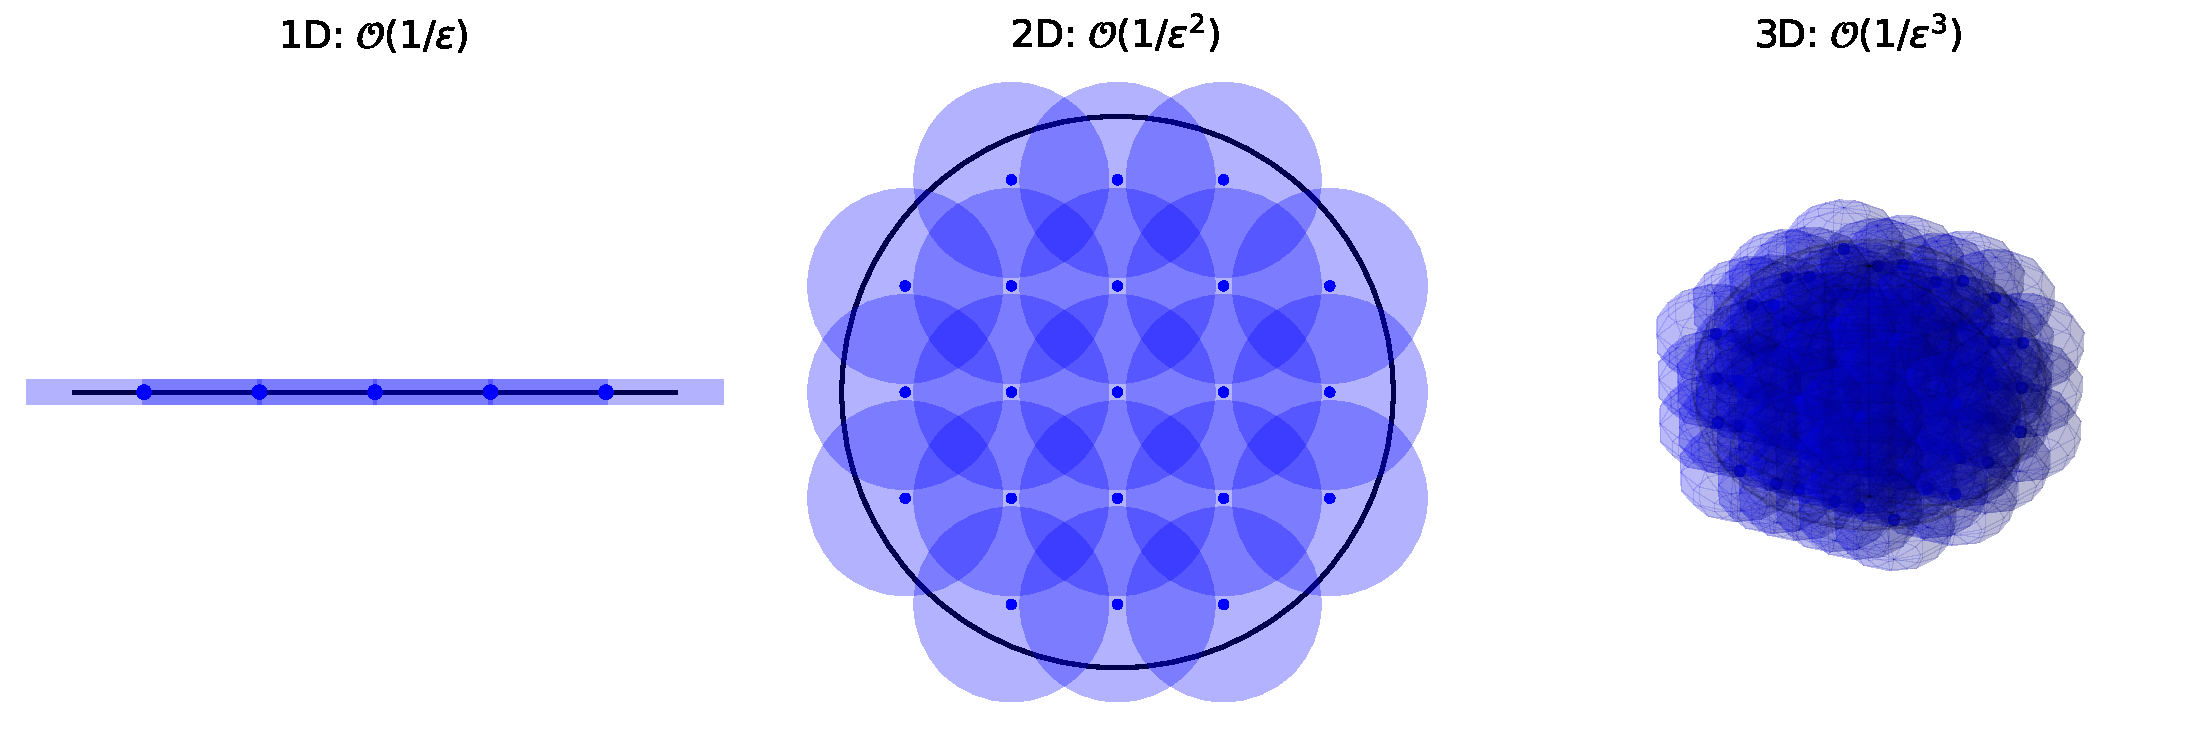
\includegraphics[width=0.95\textwidth]{epsilon_net.pdf}
\caption{Visual representation of the exponential growth of the covering number $\mathcal{N}(\mathbb{S}^{d-1}, \epsilon)$. As dimension $d$ increases, the number of samples (centers in blue) of radius $\epsilon$ required to cover the entire volume without leaving holes grows exponentially as $\mathcal{O}((1/\epsilon)^d)$.}
\label{fig:4.2}
\end{figure}

% =========================================================================
% CHAPTER 5
% =========================================================================
\chapter{The Non-Contrastive Revolution: Decorrelation and Barlow's Principle}
\label{chap:5}

The search for methods independent of negative samples led to one of the richest intersections between theoretical neurobiology and representation learning: the application of Barlow's principle. This chapter details the mathematical foundations of cross-correlation losses (Barlow Twins) and explicit covariance regularization (VICReg).

\section{Barlow's Redundancy Reduction Hypothesis (1961)}
\label{sec:5.1}

In 1961, neurobiologist Horace Barlow formulated the \textbf{efficient coding hypothesis}, proposing that the nervous system does not process sensory stimuli in the raw, but recodes them so that the activity of individual neurons is, as far as possible, statistically independent \cite{barlow1961possible}. The idea drew upon earlier work by Shannon, who had shown that natural signals such as language contain considerable redundancy: much of the signal is predictable from the rest and therefore contributes no new information in Shannon's sense. An optimal code, from this perspective, eliminates such redundancy and represents the signal using the fewest possible statistically correlated symbols.

Translating this principle to biology, Barlow observed that our environment exhibits strong spatiotemporal correlations. For example, luminance in contiguous regions of the visual field rarely changes abruptly, so transmitting every pixel or time instant independently would waste much of the neural channel's capacity on redundant information, incurring a metabolic cost the brain cannot afford. To resolve this, the sensory cortex acts as a filter that suppresses redundancy, projecting input signals onto a new space of mutually independent features. The network thus avoids expending resources on what is already predictable from the immediate context, reserving them for genuinely novel information.

\subsection{Mutual Information as the Ideal Measure of Independence}
\label{sec:5.1.1}

To formalize Barlow's redundancy reduction hypothesis, the goal is to ensure that the components of the embedding vector $Z = (z_{1}, z_{2}, \dots, z_{d})$ extracted by a model are as mutually independent as possible.

In elementary statistics, independence is often approximated by Pearson's linear correlation ($\rho$). However, its main limitation is that it only detects linear relationships. To measure dependence exhaustively and faithfully, the ideal metric is \textbf{Mutual Information} ($I$) from Shannon's information theory \cite{shannon1948mathematical}. Unlike linear correlation, mutual information captures any form of dependence (linear or nonlinear) and is invariant under invertible transformations, guaranteeing an exact measure of redundancy.

According to Shannon, the individual information of a feature $z_{i}$ is defined by its differential entropy $H(z_{i}) = \mathbb{E}[-\log p(z_{i})]$. Analogously, the joint entropy $H(z_{i}, z_{j})$ measures the total information of the pair, where $p(z_{i})$ and $p(z_{i}, z_{j})$ denote the marginal and joint population densities, respectively. Note that these formulations assume knowledge of the underlying probability law governing the data, which is strictly unobservable and must be inferred from a finite data sample.

Mutual information is then defined as the information shared by two variables or symbols of the representation:
\begin{equation}
\label{eq:5.1}
I(z_{i}; z_{j}) = H(z_{i}) + H(z_{j}) - H(z_{i}, z_{j}).
\end{equation}
If $z_{i}$ and $z_{j}$ are completely independent, their mutual information is zero, $I(z_{i}; z_{j}) = 0$, and their joint entropy equals the sum of their marginal entropies: $H(z_{i}, z_{j}) = H(z_{i}) + H(z_{j})$. This idea can be extended to the entire feature vector by constructing the mutual information matrix $\mathcal{I}(Z) \in \mathbb{R}^{d \times d}$:
\begin{equation}
\label{eq:5.2}
\mathcal{I}(Z)_{ij} = 
\begin{cases}
H(z_{i}) & \text{if } i = j, \\
I(z_{i}; z_{j}) & \text{if } i \neq j.
\end{cases}
\end{equation}

Barlow's ideal theoretically amounts to making $\mathcal{I}(Z)$ a diagonal matrix. This means no information is shared between distinct features ($I(z_{i}; z_{j}) = 0$ for $i \neq j$), while each individual neuron (recall that in our architecture each component $z_{i}$ represents the activation of a neuron in the output projection layer) retains maximum individual entropy $H(z_{i})$, thereby preventing representation collapse (\Cref{fig:5.1}).

\begin{figure}[h!]
    \centering
    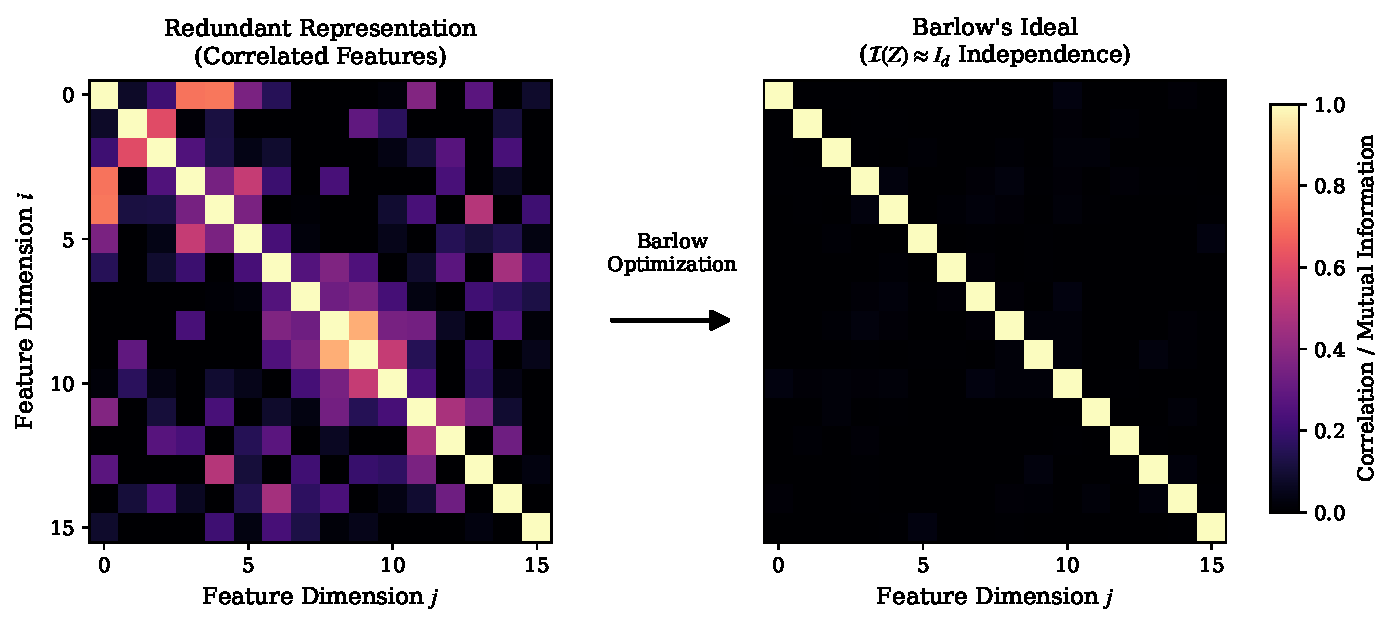
\includegraphics[width=0.9\textwidth]{heatmaps_IZ.pdf}
    \caption{Conceptual visualization of the mutual information matrix $\mathcal{I}(Z)$ (symmetric), where axes represent output neurons, or equivalently, encoding dimensions. The first matrix corresponds to a redundant representation, where significant dependencies exist between different components (non-negligible off-diagonal values). In Barlow's Ideal, the matrix exhibits a nearly diagonal structure, where components are mutually independent and each retains its maximum individual entropy.}
    \label{fig:5.1}
\end{figure}

\subsection{Jaynes' Bridge}
\label{sec:5.1.2}

Estimating mutual information and Shannon entropy is computationally intractable in high-dimensional spaces when the underlying data distribution is unknown. However, when the data follow a joint Gaussian distribution, the mutual information expression reduces to a closed form depending solely on Pearson's linear correlation coefficient ($\rho_{ij}$).

\begin{proposition}[Jaynes' Bridge]
\label{prop:5.1}
Let $(z_{i}, z_{j})$ be a pair of representations jointly distributed according to a bivariate normal distribution with Pearson correlation coefficient $\rho_{ij}$. Then the Shannon mutual information between the two variables is given by:
\begin{equation}
\label{eq:5.3}
I(z_{i}; z_{j}) = -\frac{1}{2} \log\left(1 - \rho_{ij}^{2}\right).
\end{equation}
\end{proposition}

\begin{proof}
Let $(z_{i}, z_{j})$ follow a bivariate normal distribution:
\begin{equation}
\label{eq:5.4}
\begin{pmatrix} z_{i} \\ z_{j} \end{pmatrix} \sim \mathcal{N}\left( \begin{pmatrix} \mu_{i} \\ \mu_{j} \end{pmatrix}, \Sigma \right).
\end{equation}
Recall the multivariate normal density in the general $k$-dimensional case:
\begin{equation}
\label{eq:5.5}
p(Z) = \frac{1}{\sqrt{(2\pi)^{k} \det(\Sigma)}} e^{-\frac{1}{2}(Z - \mu)^{\top} \Sigma^{-1} (Z - \mu)}.
\end{equation}
Applying the definition of Shannon differential entropy and logarithm properties:
\begin{align}
H(Z) &= \mathbb{E}[-\log p(Z)] \nonumber \\
&= \mathbb{E}\left[ \frac{1}{2}\log\left((2\pi)^{k} \det(\Sigma)\right) + \frac{1}{2}(Z - \mu)^{\top} \Sigma^{-1} (Z - \mu) \right] \label{eq:5.6} \\
&= \frac{1}{2}\log\left((2\pi)^{k} \det(\Sigma)\right) + \frac{1}{2}\mathbb{E}\left[ (Z - \mu)^{\top} \Sigma^{-1} (Z - \mu) \right]. \nonumber
\end{align}
Using $a \in \mathbb{R} \implies \tr(a) = a$, $\tr(AB) = \tr(BA)$, and $\Sigma = \mathbb{E}[(Z - \mu)(Z - \mu)^{\top}]$:
\begin{align}
\mathbb{E}\left[ (Z - \mu)^{\top} \Sigma^{-1} (Z - \mu) \right] &= \mathbb{E}\left[ \tr\left( (Z - \mu)^{\top} \Sigma^{-1} (Z - \mu) \right) \right] \nonumber \\
&= \tr\left( \Sigma^{-1} \mathbb{E}\left[ (Z - \mu)(Z - \mu)^{\top} \right] \right) \label{eq:5.7} \\
&= \tr(\Sigma^{-1} \Sigma) = \tr(I_{k}) = k. \nonumber
\end{align}
Substituting back and applying logarithm properties:
\begin{align}
H(Z) &= \frac{1}{2}\log\left((2\pi)^{k} \det(\Sigma)\right) + \frac{k}{2} \nonumber \\
&= \frac{1}{2}\log\left((2\pi)^{k} \det(\Sigma)\right) + \frac{1}{2}\log(e^{k}) \label{eq:5.8} \\
&= \frac{1}{2}\log\left((2\pi e)^{k} \det(\Sigma)\right). \nonumber
\end{align}

To evaluate the joint entropy $H(z_{i}, z_{j})$, we specialize the above formula to $k = 2$. Using the relation $\Sigma_{ij} = \rho_{ij}\sqrt{\Sigma_{ii}\Sigma_{jj}}$, we compute the determinant of the covariance matrix:
\begin{align}
\det(\Sigma) &= \Sigma_{ii}\Sigma_{jj} - \Sigma_{ij}^{2} \nonumber \\
&= \Sigma_{ii}\Sigma_{jj} - \left( \rho_{ij}\sqrt{\Sigma_{ii}\Sigma_{jj}} \right)^{2} \label{eq:5.9} \\
&= \Sigma_{ii}\Sigma_{jj} - \rho_{ij}^{2}\Sigma_{ii}\Sigma_{jj} = \Sigma_{ii}\Sigma_{jj}\left(1 - \rho_{ij}^{2}\right). \nonumber
\end{align}
Thus, the joint entropy is:
\begin{equation}
\label{eq:5.10}
H(z_{i}, z_{j}) = \frac{1}{2}\log\left( (2\pi e)^{2} \Sigma_{ii}\Sigma_{jj}(1 - \rho_{ij}^{2}) \right).
\end{equation}
Meanwhile, the marginal distributions $p(z_{i})$ and $p(z_{j})$ are univariate Gaussians ($k = 1$) with variances $\Sigma_{ii}$ and $\Sigma_{jj}$, respectively. Their individual marginal entropies are:
\begin{equation}
\label{eq:5.11}
H(z_{i}) = \frac{1}{2}\log(2\pi e \Sigma_{ii}), \qquad H(z_{j}) = \frac{1}{2}\log(2\pi e \Sigma_{jj}).
\end{equation}
Applying the definition of mutual information and algebraic properties of logarithms:
\begin{align}
I(z_{i}; z_{j}) &= H(z_{i}) + H(z_{j}) - H(z_{i}, z_{j}) \nonumber \\
&= \frac{1}{2}\log(2\pi e \Sigma_{ii}) + \frac{1}{2}\log(2\pi e \Sigma_{jj}) - \frac{1}{2}\log\left( (2\pi e)^{2}\Sigma_{ii}\Sigma_{jj}(1 - \rho_{ij}^{2}) \right) \nonumber \\
&= \frac{1}{2}\log\left( \frac{(2\pi e)^{2}\Sigma_{ii}\Sigma_{jj}}{(2\pi e)^{2}\Sigma_{ii}\Sigma_{jj}(1 - \rho_{ij}^{2})} \right) \nonumber \\
&= -\frac{1}{2}\log\left(1 - \rho_{ij}^{2}\right). \label{eq:5.12}
\end{align}
\end{proof}

Consequently, under the assumption that representations follow a multivariate Gaussian distribution, linear correlation suffices to capture all statistical dependencies. In this setting, enforcing linear decorrelation is sufficient to guarantee full statistical independence. The following corollary shows how this simplifies the optimization of the mutual information matrix $\mathcal{I}(Z)$:

\begin{corollary}[Matrix Equivalence]
\label{cor:5.1}
Let $Z \in \mathbb{R}^{d}$ be a representation vector following a multivariate normal distribution, $\mathcal{I}(Z) \in \mathbb{R}^{d \times d}$ its mutual information matrix, and $R \in \mathbb{R}^{d \times d}$ its linear correlation matrix. Under the normality hypothesis, guaranteeing statistical independence is equivalent to imposing linear decorrelation:
\begin{equation}
\label{eq:5.13}
\mathcal{I}(Z) \text{ is diagonal} \iff R = I_{d},
\end{equation}
where $I_{d}$ denotes the $d$-dimensional identity matrix.
\end{corollary}

\begin{proof}
By definition, the main diagonal elements of any correlation matrix $R$ equal unity ($R_{ii} = \rho_{ii} = 1$). For off-diagonal elements ($i \neq j$), Jaynes' Bridge (\Cref{prop:5.1}) establishes that:
\begin{equation}
\label{eq:5.14}
I(z_{i}; z_{j}) = -\frac{1}{2}\log\left(1 - \rho_{ij}^{2}\right).
\end{equation}
The matrix $\mathcal{I}(Z)$ is diagonal if and only if the mutual information between distinct features is zero, i.e., $I(z_{i}; z_{j}) = 0$ for all $i \neq j$. Setting the expression to zero yields:
\begin{equation}
\label{eq:5.15}
-\frac{1}{2}\log\left(1 - \rho_{ij}^{2}\right) = 0 \iff \log\left(1 - \rho_{ij}^{2}\right) = 0 \iff 1 - \rho_{ij}^{2} = 1 \iff \rho_{ij} = 0.
\end{equation}
Therefore, requiring $I(z_{i}; z_{j}) = 0$ for all $i \neq j$ is equivalent to imposing $\rho_{ij} = 0$ for all $i \neq j$. Since the diagonal elements of $R$ equal $1$, this condition is equivalent to $R = I_{d}$.
\end{proof}

\section{The Barlow Twins Architecture}
\label{sec:5.2}

Proposed by Zbontar et al.\ in 2021 \cite{zbontar2021barlow}, the \textbf{Barlow Twins} method translates Barlow's redundancy reduction principle from the preceding section into a practical self-supervised learning framework.

\begin{figure}[H]
    \centering
    \begin{tikzpicture}[
        node distance=1.5cm and 2cm,
        box/.style={draw, rectangle, rounded corners, minimum width=2.2cm, minimum height=1.2cm, align=center, fill=blue!5},
        img/.style={draw, rectangle, rounded corners, minimum width=1.5cm, minimum height=1.5cm, fill=orange!10, align=center},
        mat/.style={draw, rectangle, minimum width=2.5cm, minimum height=2.5cm, fill=green!5, align=center},
        arrow/.style={->, >=stealth, thick}
    ]
        \node (x) {Observation $x$};
        \node[img, above right=0.5cm and 0.8cm of x] (ya) {View $A$\\$x_1 = t^A(x)$};
        \node[img, below right=0.5cm and 0.8cm of x] (yb) {View $B$\\$x_2 = t^B(x)$};
        \node[box, right=0.8cm of ya] (enc_a) {Network\\$f_\theta$};
        \node[box, right=0.8cm of yb] (enc_b) {Network\\$f_\theta$};
        \node[right=0.6cm of enc_a] (za) {$z^A$};
        \node[right=0.6cm of enc_b] (zb) {$z^B$};
        \node[mat, right=1.2cm of za, yshift=-1.6cm] (matrix) {Cross-correlation\\$C$};
        \node[right=0.8cm of matrix, font=\Large] (identidad) {$I_d$};
        
        \draw[arrow] (x.east) to[out=0, in=180] (ya.west);
        \draw[arrow] (x.east) to[out=0, in=180] (yb.west);
        \draw[arrow] (ya) -- (enc_a);
        \draw[arrow] (yb) -- (enc_b);
        \draw[arrow] (enc_a) -- (za);
        \draw[arrow] (enc_b) -- (zb);
        \draw[arrow] (za.east) to[out=0, in=180] (matrix.150);
        \draw[arrow] (zb.east) to[out=0, in=180] (matrix.210);
        \draw[<->, >=stealth, thick, red] (matrix.east) -- node[above, text=black] {$\mathcal{L}_{\text{BT}}$} (identidad.west);
        \draw[<->, dashed, thick, gray] (enc_a.south) -- node[right, text=black, align=center, text width=2.5cm] {Shared weights} (enc_b.north);
    \end{tikzpicture}
    \caption{Architecture diagram of Barlow Twins. Two random transformations $t^A$ and $t^B$ generate distorted views of $x$. Both are processed by Siamese networks $f_\theta$ to obtain $z^A$ and $z^B$. The cross-correlation matrix $C$ is computed over the minibatch and its discrepancy from $I_d$ is minimized.}
    \label{fig:5.2}
\end{figure}

\subsection{Construction of Views and Representations}
\label{sec:5.2.1}

Given an observation $x$, two views $x_{1}$ and $x_{2}$ are generated via independent random transformations $t^{A}, t^{B}$ (e.g., cropping, masking, color jittering). Both views $x_{1} = t^{A}(x)$ and $x_{2} = t^{B}(x)$ are processed by the same network $f_{\theta}$ (shared weights), producing two vector representations in $\mathbb{R}^{d}$:
\begin{equation}
\label{eq:5.16}
z^{A} = f_{\theta}(x_{1}), \qquad z^{B} = f_{\theta}(x_{2}).
\end{equation}
In an ideal scenario where the model is completely invariant to the applied transformations, $z^{A} = z^{B}$ would hold. Over a minibatch of $N$ compatible pairs $\{(x_{1}^{(i)}, x_{2}^{(i)})\}_{i=1}^{N}$, we stack the representations of each view into a batch matrix:
\begin{equation}
\label{eq:5.17}
Z^{A}, Z^{B} \in \mathbb{R}^{N \times d}, \quad \text{where row } i \text{ of } Z^{A} \text{ is } z^{A,(i)} = f_{\theta}(x_{1}^{(i)}) \in \mathbb{R}^{d},
\end{equation}
and analogously for $Z^{B}$ with $z^{B,(i)} = f_{\theta}(x_{2}^{(i)})$. Each row is a minibatch observation; each column represents a dimension of the latent space. We denote by $z_{k}^{A,(i)}$ the $(i,k)$ entry of $Z^{A}$, i.e., the value of the $k$-th representation dimension of view $A$ for observation $i$.

\subsection{Mean Centering}
\label{sec:5.2.2}

Before speaking of correlation, the representations must be mean-centered: for each view and each dimension $k$, its empirical mean over the minibatch is subtracted:
\begin{equation}
\label{eq:5.18}
z_{k}^{A,(i)} \leftarrow z_{k}^{A,(i)} - \frac{1}{N}\sum_{m=1}^{N} z_{k}^{A,(m)}, \qquad z_{k}^{B,(i)} \leftarrow z_{k}^{B,(i)} - \frac{1}{N}\sum_{m=1}^{N} z_{k}^{B,(m)}.
\end{equation}
This centers each column of $Z^{A}$ and $Z^{B}$ to zero mean. The reason for requiring this is straightforward: if representations were not centered, the inner product between columns would be dominated by a large mean offset, masking the true covariance across dimensions. Centering guarantees that what we subsequently optimize are genuine correlations rather than uncentered second-order moments.

\subsection{The Cross-Correlation Matrix}
\label{sec:5.2.3}

With $Z^{A}, Z^{B} \in \mathbb{R}^{N \times d}$ (already column-centered), let $z_{k}^{A}, z_{l}^{B} \in \mathbb{R}^{N}$ denote the $k$-th column of $Z^{A}$ and the $l$-th column of $Z^{B}$, respectively; that is, $z_{k}^{A} = (z_{k}^{A,(1)}, \dots, z_{k}^{A,(N)})^{\top}$.

\begin{definition}[Empirical Cross-Correlation Matrix]
\label{def:5.1}
The cross-correlation matrix $C \in \mathbb{R}^{d \times d}$ is defined entrywise as the cosine similarity between the $k$-th column of $Z^{A}$ and the $l$-th column of $Z^{B}$:
\begin{equation}
\label{eq:5.19}
C_{kl} = \frac{\langle z_{k}^{A}, z_{l}^{B} \rangle}{\lVert z_{k}^{A} \rVert_{2} \lVert z_{l}^{B} \rVert_{2}} = \frac{\sum_{i=1}^{N} z_{k}^{A,(i)} z_{l}^{B,(i)}}{\sqrt{\sum_{i=1}^{N} (z_{k}^{A,(i)})^{2}} \sqrt{\sum_{i=1}^{N} (z_{l}^{B,(i)})^{2}}}, \qquad C_{kl} \in [-1, 1].
\end{equation}
Equivalently, in matrix notation: $C = (\tilde{Z}^{A})^{\top} \tilde{Z}^{B}$ after normalizing each column of $Z^{A}$ and $Z^{B}$ to unit Euclidean norm.
\end{definition}

\begin{figure}[H]
    \centering
    \resizebox{\linewidth}{!}{
    \begin{tikzpicture}[
        every node/.style={font=\footnotesize},
        mathnode/.style={font=\footnotesize, minimum width=0.6cm, minimum height=0.45cm},
        highlight/.style={fill=orange!15, draw=orange!70!black, thick},
        highlightB/.style={fill=blue!10, draw=blue!60!black, thick},
        cellhighlight/.style={fill=green!15, draw=green!50!black, thick}
    ]

    \matrix (ZA) [
        matrix of math nodes,
        nodes={mathnode},
        ampersand replacement=\&,
        left delimiter={(}, right delimiter={)},
        column sep=1pt, row sep=1pt,
        anchor=center
    ]
    {
        z_1^{A,(1)} \& \cdots \& z_k^{A,(1)} \& \cdots \& z_d^{A,(1)} \\
        z_1^{A,(2)} \& \cdots \& z_k^{A,(2)} \& \cdots \& z_d^{A,(2)} \\
        \vdots      \&        \& \vdots      \&        \& \vdots      \\
        z_1^{A,(N)} \& \cdots \& z_k^{A,(N)} \& \cdots \& z_d^{A,(N)} \\
    };
    \begin{scope}[on background layer]
        \node[highlight, fit=(ZA-1-3)(ZA-4-3), inner sep=1pt] (colA) {};
    \end{scope}
    \node[above=0.1cm of ZA] {$Z^A \in \mathbb{R}^{N \times d}$};
    \node[below=0.1cm of colA, text=orange!70!black] {dimension $k$: $\mathbf{z}_k^A$};
    \node[font=\footnotesize, text=gray!80!black, rotate=90] at ([xshift=-0.6cm]ZA.west) {$\longleftarrow$ observations $\longrightarrow$};

    \matrix (ZB) [
        matrix of math nodes,
        nodes={mathnode},
        ampersand replacement=\&,
        left delimiter={(}, right delimiter={)},
        column sep=1pt, row sep=1pt,
        anchor=center,
        right=0.6cm of ZA
    ]
    {
        z_1^{B,(1)} \& \cdots \& z_l^{B,(1)} \& \cdots \& z_d^{B,(1)} \\
        z_1^{B,(2)} \& \cdots \& z_l^{B,(2)} \& \cdots \& z_d^{B,(2)} \\
        \vdots      \&        \& \vdots      \&        \& \vdots      \\
        z_1^{B,(N)} \& \cdots \& z_l^{B,(N)} \& \cdots \& z_d^{B,(N)} \\
    };
    \begin{scope}[on background layer]
        \node[highlightB, fit=(ZB-1-3)(ZB-4-3), inner sep=1pt] (colB) {};
    \end{scope}
    \node[above=0.1cm of ZB] {$Z^B \in \mathbb{R}^{N \times d}$};
    \node[below=0.1cm of colB, text=blue!60!black] {dimension $l$: $\mathbf{z}_l^B$};

    \matrix (C) [
        matrix of math nodes,
        nodes={mathnode},
        ampersand replacement=\&,
        left delimiter={(}, right delimiter={)},
        column sep=1pt, row sep=1pt,
        anchor=center,
        right=0.6cm of ZB
    ]
    {
        C_{11} \& \cdots \& C_{1l} \& \cdots \& C_{1d} \\
        \vdots \&        \& \vdots \&        \& \vdots \\
        C_{k1} \& \cdots \& C_{kl} \& \cdots \& C_{kd} \\
        \vdots \&        \& \vdots \&        \& \vdots \\
        C_{d1} \& \cdots \& C_{dl} \& \cdots \& C_{dd} \\
    };
    \begin{scope}[on background layer]
        \node[cellhighlight, fit=(C-3-3), inner sep=1pt] (cellKL) {};
    \end{scope}
    \node[above=0.1cm of C] {$C \in \mathbb{R}^{d \times d}$};

    \node[
        below=0.6cm of C,
        anchor=center
    ] (dotprod) {
        \textcolor{green!50!black}{$C_{kl}$} $= \dfrac{\langle {\mathbf{z}_k^A}, {\mathbf{z}_l^B} \rangle}
        {\|{\mathbf{z}_k^A}\|_2 \, \|{\mathbf{z}_l^B}\|_2}$
    };

    \end{tikzpicture}
    }
    \caption{Construction of the cross-correlation matrix $C$ via normalized inner product (cosine similarity) between columns of $Z^A$ and $Z^B$.}
    \label{fig:5.3}
\end{figure}




\begin{definition}[Barlow Twins Loss Function]
\label{def:5.2}
The loss penalizes the discrepancy between $C$ and the identity matrix $I_{d}$:
\begin{equation}
\label{eq:5.20}
\mathcal{L}_{\text{BT}} = \underbrace{\sum_{k=1}^{d} (1 - C_{kk})^{2}}_{\text{Invariance}} + \lambda \underbrace{\sum_{k=1}^{d} \sum_{l \neq k} C_{kl}^{2}}_{\text{Redundancy}},
\end{equation}
where $\lambda > 0$ is a hyperparameter weighting the two loss objectives. Analogously to how the margin in contrastive losses regulates repulsion between negative samples, here $\lambda$ modulates repulsion between features.
\end{definition}

Each term of $\mathcal{L}_{\text{BT}}$ has a clear geometric interpretation derived from the construction of $C$:
\begin{itemize}
    \item \textbf{Invariance ($C_{kk} \to 1$):} $C_{kk}$ is the cosine similarity between column $k$ of $Z^{A}$ and column $k$ of $Z^{B}$, i.e., between the values that dimension $k$ assumes in view $A$ and in view $B$ across the entire minibatch. Forcing $C_{kk} \to 1$ requires both columns to be positively proportional in $\mathbb{R}^{N}$; by the Cauchy-Schwarz inequality, this holds if and only if $z_{k}^{A} = c \cdot z_{k}^{B}$ with $c > 0$, meaning that the network extracts the same information in dimension $k$ regardless of the view processed.
    \item \textbf{Redundancy reduction ($C_{kl} \to 0, \, k \neq l$):} During training, the views differ ($Z^{A} \neq Z^{B}$), so $C_{kl}$ captures the cross-correlation between dimension $k$ of view $A$ and dimension $l$ of view $B$. Forcing $C_{kl} \to 0$ amounts to imposing $\langle z_{k}^{A}, z_{l}^{B} \rangle \to 0$, i.e., cross-orthogonality between distinct dimensions of the two views. Each dimension is thus forced to encode information not captured by the others, spreading semantic variance across all of $\mathbb{R}^{d}$ in accordance with Barlow's principle.
\end{itemize}

The empirical matrix $C$ approximates, on each minibatch, the population cross-correlation $C_{kl} = \mathbb{E}[z_{k}^{A} z_{l}^{B}] / \sqrt{\mathbb{E}[(z_{k}^{A})^{2}]\mathbb{E}[(z_{l}^{B})^{2}]}$ defined over the positive-pair distribution $p_{\text{pos}}(x_{1}, x_{2})$. Barlow Twins employs cross-correlation rather than autocorrelation precisely because, during training, $Z^{A} \neq Z^{B}$; by operating on $C$, the method simultaneously measures and minimizes inter-view discrepancy along the diagonal and inter-feature redundancy off the diagonal.

The connection with Barlow's theory becomes exact in the limit of perfect invariance. When the model assimilates both views identically ($Z^{A} = Z^{B} = Z$), each pair of columns collapses to a single vector ($z_{k}^{A} = z_{k}^{B} = z_{k}$), and the cross-correlation $C$ reduces to Pearson's autocorrelation matrix $R$ of \Cref{sec:5.1}. In that limit, forcing $C \to I_{d}$ is strictly equivalent to imposing $R \to I_{d}$, achieving the decorrelation required by the original principle.

\section{VICReg: Decoupling Variance, Invariance, and Covariance}
\label{sec:5.3}

Choosing the cross-correlation matrix $C$ as the central optimization object in Barlow Twins entails certain design limitations. Recall that each entry $C_{kl}$ is obtained by dividing the inner product between columns $z_{k}^{A}$ and $z_{l}^{B}$ by the product of their Euclidean norms. This causes the optimization objective to ignore the scale of the representations, focusing solely on directions.

\begin{proposition}[Scale Invariance of $C$]
\label{prop:5.2}
Let $C$ be the cross-correlation matrix defined in \Cref{sec:5.2}. For any positive dimension-wise rescaling $z_{j} \mapsto \alpha_{j} z_{j}$ with $\alpha_{j} > 0$, the matrix $C$ remains unaltered.
\end{proposition}

\begin{proof}
Let $\tilde{z}_{k}^{A} = \alpha_{k} z_{k}^{A}$ and $\tilde{z}_{l}^{B} = \alpha_{l} z_{l}^{B}$ be the rescaled columns. Then:
\begin{equation}
\label{eq:5.21}
\tilde{C}_{kl} = \frac{\langle \alpha_{k} z_{k}^{A}, \alpha_{l} z_{l}^{B} \rangle}{\lVert \alpha_{k} z_{k}^{A} \rVert_{2} \lVert \alpha_{l} z_{l}^{B} \rVert_{2}} = \frac{\alpha_{k} \alpha_{l} \langle z_{k}^{A}, z_{l}^{B} \rangle}{\alpha_{k} \lVert z_{k}^{A} \rVert_{2} \alpha_{l} \lVert z_{l}^{B} \rVert_{2}} = C_{kl}.
\end{equation}
The factors $\alpha_{k}$ and $\alpha_{l}$ cancel out exactly due to normalization.
\end{proof}

Consequently, the Barlow Twins formulation based on the cross-correlation matrix $C$ exhibits two fundamental issues limiting its regularization capacity:
\begin{enumerate}
    \item \textbf{Dimensional collapse due to lack of scale sensitivity.}
    \item \textbf{Objective coupling (entanglement).}
\end{enumerate}

Regarding the first issue, \Cref{prop:5.2} implies that $C$ discards all information about the scale of the dimensions of $\mathcal{Z}$. In particular, reducing the variance of a dimension $j$ to an arbitrarily small value does not alter the diagonal elements $C_{jj}$, as they are normalized. Recall that if a dimension has zero variance, the network is emitting the exact same numerical value for all images along that coordinate---precisely the empirical manifestation of dimensional collapse. A collapsed dimension (whose variance tends to zero because it encodes no useful information) can still maintain an optimal value $C_{jj} \approx 1$ as long as the residual numerical fluctuations in $z_{j}^{A}$ and $z_{j}^{B}$ remain aligned. The loss $\mathcal{L}_{\text{BT}}$ does not distinguish between a dimension with unit variance and one with negligible variance; both contribute identically to the diagonal of $C$. Thus, $\mathcal{L}_{\text{BT}}$ lacks an explicit mechanism to guarantee that all dimensions of $\mathcal{Z}$ maintain sufficient dispersion.

The second issue arises from condensing the invariance ($C_{kk} \to 1$) and decorrelation ($C_{kl} \to 0$) objectives into a single normalized object $C$. Because both terms share the same normalization denominator, they cannot be treated independently: any perturbation propagates simultaneously to the diagonal and off-diagonal entries of $C$, coupling two conceptually distinct objectives \cite{bardes2022vicreg}.

\textbf{VICReg} (Variance-Invariance-Covariance Regularization), proposed by Bardes, Ponce, and LeCun in 2022 \cite{bardes2022vicreg}, resolves these limitations by explicitly decoupling invariance, dimensional dispersion, and feature independence over an object that retains the scale information discarded by $C$.

\subsection{From Cross-Correlation to Covariance}
\label{sec:5.3.1}

\begin{definition}[Empirical Covariance Matrix]
\label{def:5.3}
Let $Z \in \mathbb{R}^{N \times d}$ be an embedding matrix corresponding to a batch of $N$ observations, and let $\bar{z} = \frac{1}{N}\sum_{i=1}^{N} z^{(i)} \in \mathbb{R}^{d}$ be its mean vector. The empirical covariance matrix is defined as:
\begin{equation}
\label{eq:5.22}
\Sigma_{\mathcal{Z}} = \frac{1}{N - 1}\sum_{i=1}^{N} (z^{(i)} - \bar{z})(z^{(i)} - \bar{z})^{\top} = \frac{1}{N - 1}(Z - \bar{Z})^{\top}(Z - \bar{Z}) \in \mathbb{R}^{d \times d},
\end{equation}
where $\bar{Z} \in \mathbb{R}^{N \times d}$ denotes the matrix whose $N$ rows are all equal to $\bar{z}^{\top}$. The entry $(\Sigma_{\mathcal{Z}})_{kl} = \Cov(z_{k}, z_{l})$ is the empirical covariance between dimensions $k$ and $l$ across the batch, and in particular $(\Sigma_{\mathcal{Z}})_{jj} = \Var(z_{j})$ is the empirical variance of dimension $j$.
\end{definition}

In the invariance limit analyzed at the end of \Cref{sec:5.2} ($Z^{A} = Z^{B} = Z$), the cross-correlation $C$ reduces to the autocorrelation matrix $R$ of a single view. The relationship between $R$ and the covariance $\Sigma_{\mathcal{Z}}$ of the same random vector is:
\begin{equation}
\label{eq:5.23}
R_{kl} = \frac{(\Sigma_{\mathcal{Z}})_{kl}}{\sqrt{(\Sigma_{\mathcal{Z}})_{kk}}\sqrt{(\Sigma_{\mathcal{Z}})_{ll}}}.
\end{equation}
\Cref{eq:5.23} shows that $R$ (and by extension $C$ in the invariance limit) can be reconstructed from $\Sigma_{\mathcal{Z}}$, whereas the inverse operation is impossible: given $R$, one cannot recover the variances eliminated by normalization:
\[
C = \begin{pmatrix}
1 & C_{12} & \cdots & C_{1d} \\
C_{21} & 1 & \cdots & C_{2d} \\
\vdots & \vdots & \ddots & \vdots \\
C_{d1} & C_{d2} & \cdots & 1
\end{pmatrix}, \qquad
\Sigma_{\mathcal{Z}} = \begin{pmatrix}
\sigma_{1}^{2} & \Sigma_{12} & \cdots & \Sigma_{1d} \\
\Sigma_{21} & \sigma_{2}^{2} & \cdots & \Sigma_{2d} \\
\vdots & \vdots & \ddots & \vdots \\
\Sigma_{d1} & \Sigma_{d2} & \cdots & \sigma_{d}^{2}
\end{pmatrix}.
\]
The diagonal of $\Sigma_{\mathcal{Z}}$ explicitly retains the individual variances $\sigma_{j}^{2} = (\Sigma_{\mathcal{Z}})_{jj}$, while the diagonal of $C$ is identically $1$ by construction. Thus, $\Sigma_{\mathcal{Z}}$ contains strictly more information than $R$.

\subsection{Invariance Term}
\label{sec:5.3.2}

As introduced in \Cref{chap:3}, the primary objective of any Joint Embedding Architecture is invariance: the network must learn that representations of two views of the same observation should be close ($z^{A} \approx z^{B}$). To capture both direction and magnitude without normalization, VICReg recovers the positive loss $\mathcal{L}_{\text{pos}}$ defined in \Cref{chap:3}.

\begin{definition}[VICReg Invariance Term]
\label{def:5.4}
Given two batches of embeddings $Z^{A}, Z^{B} \in \mathbb{R}^{N \times d}$ generated from positive pairs $\{(x_{1}^{(i)}, x_{2}^{(i)})\}_{i=1}^{N}$, the invariance term is defined as the mean squared error between the representations of each pair:
\begin{equation}
\label{eq:5.24}
\mathcal{L}_{\text{pos}}(Z^{A}, Z^{B}) = \frac{1}{N}\sum_{i=1}^{N} \lVert z^{A,(i)} - z^{B,(i)} \rVert_{2}^{2}.
\end{equation}
\end{definition}

\subsection{Variance Term}
\label{sec:5.3.3}

VICReg resolves the scale blind spot by introducing a hinge regularization term that acts directly on the diagonal of the covariance matrix $\Sigma_{\mathcal{Z}}$, i.e., the individual variances $\{(\Sigma_{\mathcal{Z}})_{jj}\}_{j=1}^{d}$ of each dimension of the latent space.

\begin{definition}[VICReg Variance Term]
\label{def:5.5}
Let $Z \in \mathbb{R}^{N \times d}$ be a batch of embeddings and let $\sigma_{j}(Z) = \sqrt{(\Sigma_{\mathcal{Z}})_{jj}}$, where $(\Sigma_{\mathcal{Z}})_{jj}$ is the empirical variance of dimension $j$. The variance term in the VICReg loss is defined by aggregating these values across all dimensions of $\mathcal{Z}$ whenever dispersion is insufficient:
\begin{equation}
\label{eq:5.25}
\mathcal{L}_{\text{var}}(Z) = \frac{1}{d}\sum_{j=1}^{d} \max\left(0, 1 - \sigma_{j}(Z)\right).
\end{equation}
\end{definition}

The $\max$ function sets a threshold $\gamma = 1$ on the standard deviation of each dimension:
\begin{itemize}
    \item If $\sigma_{j}(Z) < 1$, dimension $j$ has insufficient dispersion in the batch and the term becomes active: $\max(0, 1 - \sigma_{j}) = 1 - \sigma_{j} > 0$. The derivative $\partial \mathcal{L}_{\text{var}} / \partial \sigma_{j} = -1/d$ injects a gradient that expands representations along that dimension, counteracting the contractive force of $\mathcal{L}_{\text{pos}}$.
    \item If $\sigma_{j}(Z) \geq 1$, the dimension already possesses sufficient dispersion and deactivates: $\max(0, 1 - \sigma_{j}) = 0$.
\end{itemize}

\subsection{Covariance Term}
\label{sec:5.3.4}

The third objective is redundancy reduction. Following Barlow's hypothesis \cite{barlow1961possible}, dimensions of the latent space must encode independent information. VICReg pursues this goal by operating on the unnormalized covariance off-diagonal entries.

\begin{definition}[VICReg Covariance Term]
\label{def:5.6}
Let $\Sigma_{\mathcal{Z}} \in \mathbb{R}^{d \times d}$ be the empirical batch covariance matrix defined in \Cref{eq:5.22}. The covariance term in the VICReg loss aggregates the squared off-diagonal entries:
\begin{equation}
\label{eq:5.26}
\mathcal{L}_{\text{cov}}(Z) = \frac{1}{d}\sum_{k=1}^{d} \sum_{l \neq k} (\Sigma_{\mathcal{Z}})_{kl}^{2}.
\end{equation}
\end{definition}

\begin{remark}
\label{rem:5.1}
As established at the beginning of the chapter, Jaynes' Bridge shows that, under the normality hypothesis, mutual information between two dimensions depends exclusively on Pearson's correlation coefficient: $I(z_{k}; z_{l}) = -\frac{1}{2}\log(1 - \rho_{kl}^{2})$. Since the correlation coefficient is expressed as:
\begin{equation}
\label{eq:5.27}
\rho_{kl} = \frac{(\Sigma_{\mathcal{Z}})_{kl}}{\sqrt{(\Sigma_{\mathcal{Z}})_{kk}(\Sigma_{\mathcal{Z}})_{ll}}},
\end{equation}
and the variance term ensures $(\Sigma_{\mathcal{Z}})_{kk} > 0$, we have $\rho_{kl} = 0$ if and only if $(\Sigma_{\mathcal{Z}})_{kl} = 0$. Therefore, forcing $(\Sigma_{\mathcal{Z}})_{kl} \to 0$ via $\mathcal{L}_{\text{cov}}(Z)$ is equivalent to forcing $\rho_{kl} \to 0$, which by Jaynes' Bridge guarantees $I(z_{k}; z_{l}) \to 0$ under normality.
\end{remark}

\subsection{The Complete VICReg Loss Function}
\label{sec:5.3.5}

\begin{definition}[VICReg Loss Function]
\label{def:5.7}
The total VICReg loss is defined as the inner product between the hyperparameter weight vector $\mu$ and the vector of individual loss components $L(Z^{A}, Z^{B})$:
\begin{align}
\mathcal{L}_{\text{VICReg}} &= \langle \mu, L(Z^{A}, Z^{B}) \rangle \nonumber \\
&= \mu_{1}\mathcal{L}_{\text{pos}}(Z^{A}, Z^{B}) + \mu_{2}\left[\mathcal{L}_{\text{var}}(Z^{A}) + \mathcal{L}_{\text{var}}(Z^{B})\right] + \mu_{3}\left[\mathcal{L}_{\text{cov}}(Z^{A}) + \mathcal{L}_{\text{cov}}(Z^{B})\right], \label{eq:5.28}
\end{align}
where $\mu = (\mu_{1}, \mu_{2}, \mu_{3})^{\top}$ with $\mu_{1}, \mu_{2}, \mu_{3} > 0$ weighting each component.
\end{definition}

\begin{figure}[H]
\centering
\resizebox{\linewidth}{!}{
\begin{tikzpicture}[
    node distance=1cm,
    inputbox/.style={draw, rectangle, rounded corners, minimum width=1.8cm, minimum height=0.7cm, align=center, fill=gray!5, font=\footnotesize},
    matbox/.style={draw, rectangle, rounded corners, minimum width=2.5cm, minimum height=1cm, align=center, fill=green!5, font=\footnotesize},
    termbox/.style={draw, rectangle, rounded corners, minimum width=1.8cm, minimum height=0.9cm, align=center, font=\footnotesize},
    arrow/.style={->, >=stealth, thick}
]

% ===== BARLOW TWINS =====
\node[font=\small\bfseries\sffamily] (bt_title) at (0, 0) {$\mathcal{L}_{\text{BT}}$};
\node[inputbox] (bt_input) at (0, -1.2) {$Z^A, Z^B$};
\node[matbox] (bt_C) at (0, -3) {Cross-correlation $C$\\{\scriptsize normalized: $C_{kl} \in [-1,1]$}};
\node[termbox, fill=orange!12] (bt_inv) at (-1.8, -5) {$C_{kk} \to 1$\\{\scriptsize Invariance}};
\node[termbox, fill=blue!10] (bt_red) at (1.8, -5) {$C_{kl} \to 0$\\{\scriptsize Redundancy}};

\draw[arrow] (bt_input) -- (bt_C);
\draw[arrow] (bt_C) to[out=-150, in=90] (bt_inv);
\draw[arrow] (bt_C) to[out=-30, in=90] (bt_red);

\begin{scope}[on background layer]
    \node[draw=gray, dashed, rounded corners, fit=(bt_inv)(bt_red), inner sep=8pt, fill=gray!3] {};
\end{scope}

% ===== SEPARATOR =====
\draw[dashed, gray!50, thick] (3.75, 0.5) -- (3.75, -7.5);

% ===== VICREG =====
\node[font=\small\bfseries\sffamily] (vic_title) at (9, 0) {$\mathcal{L}_{\text{VICReg}}$};
\node[inputbox] (vic_input) at (9, -1.2) {$Z^A, Z^B$};

\node[matbox] (vic_sigma) at (10.5, -3) {Covariance $\Sigma_\mathcal{Z}$\\{\scriptsize $\Sigma_{Z^A}, \Sigma_{Z^B}$}};

\node[termbox, fill=orange!12] (vic_s) at (6, -5) {$\mathcal{L}_{\text{pos}}(Z^A, Z^B)$\\{\scriptsize Invariance}};
\node[termbox, fill=red!10] (vic_v) at (9, -5) {$\mathcal{L}_{\text{var}}(Z)$\\{\scriptsize Variance}};
\node[termbox, fill=blue!10] (vic_c) at (12, -5) {$\mathcal{L}_{\text{cov}}(Z)$\\{\scriptsize Covariance}};

\draw[arrow] (vic_input.south) to[out=-150, in=90] (vic_s.north);
\draw[arrow] (vic_input.south) to[out=-30, in=90] (vic_sigma.north);

\draw[arrow] (vic_sigma.south) to[out=-150, in=90] (vic_v.north);
\draw[arrow] (vic_sigma.south) to[out=-30, in=90] (vic_c.north);

\begin{scope}[on background layer]
    \node[draw=gray, dashed, rounded corners, fit=(vic_s)(vic_v)(vic_c), inner sep=10pt, fill=gray!3] {};
\end{scope}

\end{tikzpicture}
}
\caption{Comparison of regularizations. Left: Barlow Twins couples invariance and redundancy reduction through the normalized cross-correlation matrix $C$. Right: VICReg decouples invariance ($\mathcal{L}_{\text{pos}}$), variance ($\mathcal{L}_{\text{var}}$), and covariance ($\mathcal{L}_{\text{cov}}$), acting on the unnormalized covariance matrix $\Sigma_\mathcal{Z}$.}
\label{fig:5.4}
\end{figure}

\section{Limitations: Dependence on the Gaussian Hypothesis}
\label{sec:5.4}

All the theory presented in this chapter rests upon Jaynes' Bridge, which establishes the equivalence between linear decorrelation and statistical independence \textit{only when the representations follow a multivariate normal distribution}. In practice, this hypothesis is not automatically satisfied. Deep nonlinear networks can produce complex, multimodal distributions or higher-order nonlinear dependencies that Pearson correlation fails to capture. In such scenarios, two dimensions may exhibit zero linear correlation ($\rho_{kl} = 0$) while maintaining positive mutual information $I(z_{k}; z_{l}) > 0$, invalidating the equivalence of Jaynes' Bridge. Consequently, the redundancy reduction achieved by Barlow Twins and VICReg is, in the general case, only a second-order approximation to Barlow's ideal, exact solely under normality.

% =========================================================================
% CHAPTER 6
% =========================================================================
\chapter{World Models}
\label{chap:6}

In \Cref{chap:5} we showed how Barlow Twins and VICReg learn representations without resorting to negative samples by directly regularizing second-order moments. However, both methods operate on static pairs of views of the same observation: they do not account for the temporal evolution of the environment. Once we wish to build a system capable of predicting how conceptual representations evolve over time, the symmetric architecture of two encoders with shared weights becomes structurally insufficient.

This transition---from static representation learning \cite{bengio2013representation} to processes that emulate abstract reasoning over dynamics \cite{lecun2022path,lecun2025objectives}---constitutes the central conceptual leap of this chapter. The key element is the introduction of a new component, the \textbf{predictor} $g_{\phi}$, which transforms the Joint Embedding architecture into a \textbf{World Model} capable of simulating transitions in representation space. As we shall see, this structural shift reopens the collapse problem (\Cref{sec:3.2}) in forms that the matrix regularizations of \Cref{chap:5} were not designed to handle.

\section{World Models (Temporal JEPAs)}
\label{sec:6.1}

Structurally, moving from the symmetric architectures of \Cref{chap:5} to a World Model introduces a fundamental asymmetry. In Barlow Twins and VICReg (\Cref{fig:5.2}), the two network branches share the same encoder $f_{\theta}$ and play interchangeable roles: there is no notion of ``before'' and ``after.'' In a World Model, by contrast, the architecture comprises two functionally distinct components: an \textbf{encoder} that compresses sensory observations into abstract representations, and a \textbf{predictor} that simulates the dynamic transition of the environment within representation space.

\begin{definition}[World Model or Temporal JEPA]
\label{def:6.1}
A World Model consists of two main components:
\begin{enumerate}
    \item \textbf{Encoder ($f_{\theta}$):} A differentiable mapping that projects the real-world observation to the abstract state:
    \begin{equation}
    \label{eq:6.1}
    z_{t} = f_{\theta}(o_{t}) \in \mathcal{Z} \subseteq \mathbb{R}^{d}.
    \end{equation}
    \item \textbf{Predictor ($g_{\phi}$):} A mapping $g_{\phi} \colon \mathcal{Z} \to \mathcal{Z}$ (optionally conditioned on an action $a_{t}$) that models the physical transition of the environment, predicting the abstract representation of the next state from the representation of the current state:
    \begin{equation}
    \label{eq:6.2}
    \hat{z}_{t+1} = g_{\phi}(z_{t}) \in \mathcal{Z} \subseteq \mathbb{R}^{d},
    \end{equation}
    where $\theta$ and $\phi$ are the optimizable parameters of the encoder and predictor, respectively.
\end{enumerate}
\end{definition}

\begin{figure}[H]
\centering
\resizebox{\linewidth}{!}{
\begin{tikzpicture}[
    every node/.style={font=\footnotesize},
    box/.style={draw=blue!40!black, rectangle, rounded corners=4pt, minimum width=2.2cm, minimum height=1.0cm, align=center, fill=blue!8, thick},
    predbox/.style={draw=violet!40!black, rectangle, rounded corners=4pt, minimum width=2.2cm, minimum height=1.0cm, align=center, fill=violet!12, thick},
    obs/.style={draw=gray!45!black, rectangle, rounded corners=4pt, minimum width=1.8cm, minimum height=1.0cm, align=center, fill=gray!8, thick},
    lossbox/.style={draw=red!40!black, rectangle, rounded corners=4pt, fill=red!8, thick, minimum width=3.4cm, minimum height=1.2cm, align=center},
    arrow/.style={->, >=stealth, line width=1.2pt, black!75}
]

    \node[obs] (ot) {Observation\\$o_t$};
    \node[box, right=1.0cm of ot] (enc_t) {Encoder\\$f_\theta$};
    \node[right=0.8cm of enc_t] (zt) {$z_t$};
    \node[predbox, right=1.0cm of zt] (pred) {Predictor\\$g_\phi$};
    \node[right=0.8cm of pred] (zhat) {$\hat{z}_{t+1}$};

    \node[obs, below=1.8cm of ot] (ot1) {Observation\\$o_{t+1}$};
    \node[box, right=1.0cm of ot1] (enc_t1) {Encoder\\$f_\theta$};
    \node[right=0.8cm of enc_t1] (zt1) {$z_{t+1}$};

    \node[lossbox, right=1.5cm of zhat, yshift=-1.4cm] (loss_asym) {Prediction Loss\\$\mathcal{L}_{\text{pred}} = \|\hat{z}_{t+1} - z_{t+1}\|_2^2$};

    \draw[arrow] (ot) -- (enc_t);
    \draw[arrow] (enc_t) -- (zt);
    \draw[arrow] (zt) -- (pred);
    \draw[arrow] (pred) -- (zhat);

    \draw[arrow] (ot1) -- (enc_t1);
    \draw[arrow] (enc_t1) -- (zt1);

    \draw[arrow] (zhat.east) to[out=0, in=180] (loss_asym.west);
    \draw[arrow] (zt1.east) to[out=0, in=180] (loss_asym.west);

    \draw[<->, dashed, line width=1.0pt, gray!70] (enc_t.south) -- node[left, text=black, align=center, font=\scriptsize] {shared\\weights} (enc_t1.north);

    \begin{scope}[on background layer]
        \node[draw=orange!30, fill=orange!5, dashed, thick, rounded corners=8pt, fit=(zt) (pred) (zhat), inner sep=6pt] (pred_zone) {};
        \node[text=orange!80!black, font=\scriptsize\bfseries, above=0.05cm of pred_zone] {Prediction in representation space};
    \end{scope}
\end{tikzpicture}
}
\caption{Base JEPA Architecture for World Models. Given observations $o_t$ and $o_{t+1}$, encoders $f_\theta$ map them to representations $z_t$ and $z_{t+1}$. The predictor $g_\phi$ forecasts $\hat{z}_{t+1}$ from $z_t$ in latent space.}
\label{fig:6.1}
\end{figure}

However, this formulation alone does not solve the collapse problem (\Cref{sec:3.2}): if the encoder $f_{\theta}$ projects all observations to a single constant vector $z_{t} = c$ for all $t$, the predictor $g_{\phi}$ can simply learn the identity function $g_{\phi}(c) = c$, causing the prediction loss $\lVert \hat{z}_{t+1} - z_{t+1} \rVert_{2}^{2}$ to vanish trivially. Regularizing the space $\mathcal{Z}$ to prevent this degeneration remains the central challenge.

\section{The Temporal Extension of VICReg and Its Instability (PLDM)}
\label{sec:6.2}

The first strategy historically explored to regularize a World Model was the most direct: extending VICReg regularization to the sequential setting. The \textbf{PLDM} (Predictive Latent Dynamics Model) architecture, proposed by Sobal et al.\ in 2022 \cite{sobal2022joint}, adopted this path. In the static setting of \Cref{chap:5}, batch representations are organized into a two-dimensional matrix $Z \in \mathbb{R}^{N \times d}$. Upon incorporating temporal evolution, however, a batch of trajectories is represented by a three-dimensional tensor $Z \in \mathbb{R}^{N \times T \times d}$, where $N$ is the batch size, $T$ is the temporal sequence length, and $d$ is the latent space dimensionality.

This transition from matrix to tensor multiplies the required VICReg terms. To prevent representation collapse, regularization can no longer be restricted to a single axis of variation. The variance and covariance framework must now be applied along two independent axes of the tensor structure: \textbf{spatially} (across the batch dimension $N$, preventing distinct trajectories from collapsing onto each other) and \textbf{temporally} (along the time dimension $T$, preventing a single trajectory from collapsing to a constant state over time).

Thus, for a batch of trajectories indexed by $i \in \{1, \dots, N\}$ and time steps $t \in \{1, \dots, T\}$, denoting true embeddings as $z_{t}^{(i)} = f_{\theta}(o_{t}^{(i)})$ and predictor outputs as $\hat{z}_{t+1}^{(i)} = g_{\phi}(z_{t}^{(i)}, a_{t}^{(i)})$, the total PLDM loss for jointly training the encoder $f_{\theta}$ and predictor $g_{\phi}$ comprises seven coupled loss terms:
\begin{equation}
\label{eq:6.3}
\mathcal{L}_{\text{PLDM}} = \mathcal{L}_{\text{pred}} + \alpha \mathcal{L}_{\text{var}} + \beta \mathcal{L}_{\text{cov}} + \gamma \mathcal{L}_{\text{time-sim}} + \zeta \mathcal{L}_{\text{time-var}} + \nu \mathcal{L}_{\text{time-cov}} + \mu \mathcal{L}_{\text{IDM}},
\end{equation}
where the individual terms are formally defined as follows:
\begin{enumerate}
    \item \textbf{Prediction Loss ($\mathcal{L}_{\text{pred}}$):} Mean squared error between predictions and true future state representations:
    \begin{equation}
    \label{eq:6.4}
    \mathcal{L}_{\text{pred}} = \frac{1}{N(T - 1)} \sum_{i=1}^{N} \sum_{t=1}^{T-1} \lVert \hat{z}_{t+1}^{(i)} - z_{t+1}^{(i)} \rVert_{2}^{2}.
    \end{equation}
    \item \textbf{Spatial Variance ($\mathcal{L}_{\text{var}}$):} Prevents spatial collapse by forcing the variance of each feature across the batch dimension $N$ to exceed $1$, directly inheriting the role of the VICReg variance term (\Cref{def:5.5}).
    \item \textbf{Spatial Covariance ($\mathcal{L}_{\text{cov}}$):} Minimizes feature covariance across the batch to reduce spatial redundancy, analogously to the VICReg covariance term (\Cref{def:5.6}).
    \item \textbf{Temporal Variance ($\mathcal{L}_{\text{time-var}}$):} Prevents temporal collapse by forcing representations to vary over time within each trajectory (applying the VICReg variance hinge along the temporal dimension $T$).
    \item \textbf{Temporal Covariance ($\mathcal{L}_{\text{time-cov}}$):} Minimizes feature covariance across the temporal dimension $T$.
    \item \textbf{Temporal Similarity ($\mathcal{L}_{\text{time-sim}}$):} Enforces smoothness along temporal trajectories by penalizing abrupt consecutive changes:
    \begin{equation}
    \label{eq:6.5}
    \mathcal{L}_{\text{time-sim}} = \frac{1}{N(T - 1)} \sum_{i=1}^{N} \sum_{t=1}^{T-1} \lVert z_{t}^{(i)} - z_{t+1}^{(i)} \rVert_{2}^{2}.
    \end{equation}
    \item \textbf{Inverse Dynamics Model Loss ($\mathcal{L}_{\text{IDM}}$):} In action-conditioned models where $\hat{z}_{t+1}^{(i)} = g_{\phi}(z_{t}^{(i)}, a_{t}^{(i)})$, an auxiliary neural network $\idm(\cdot, \cdot)$ is introduced inside the loss function to reconstruct the executed action $a_{t}^{(i)}$ solely from contiguous state representations $z_{t}^{(i)}$ and $z_{t+1}^{(i)}$:
    \begin{equation}
    \label{eq:6.6}
    \mathcal{L}_{\text{IDM}} = \frac{1}{N(T - 1)} \sum_{i=1}^{N} \sum_{t=1}^{T-1} \lVert \hat{a}_{t}^{(i)} - a_{t}^{(i)} \rVert_{2}^{2}, \qquad \text{where } \hat{a}_{t}^{(i)} = \idm\left(z_{t}^{(i)}, z_{t+1}^{(i)}\right).
    \end{equation}
\end{enumerate}

\section{Conflicting Gradient Dynamics and Intractability}
\label{sec:6.3}

Optimizing the PLDM loss entails severe practical challenges: the large number of competing objectives induces interference among their gradients \cite{yu2020gradient} and requires an expensive hyperparameter search in $(\alpha, \beta, \gamma, \zeta, \nu, \mu) \in \mathbb{R}_{+}^{6}$ to calibrate term weights \cite{sobal2025learning}. Furthermore, the IDM term increases system complexity by embedding an entire auxiliary neural network inside the loss function itself.

\subsection*{Gradient Interference}

Several loss terms pursue directly opposing geometric objectives along the temporal axis:
\begin{itemize}
    \item The \textbf{temporal similarity term} $\mathcal{L}_{\text{time-sim}}$ acts as a contractive attractive force attempting to pull $z_{t}$ and $z_{t+1}$ together to produce smooth trajectories.
    \item The \textbf{temporal variance term} $\mathcal{L}_{\text{time-var}}$ acts as an expansive force attempting to push $z_{t}$ and $z_{t+1}$ apart so the trajectory does not collapse to a constant point in $\mathcal{Z}$.
\end{itemize}
Consequently, their respective gradients with respect to the encoder parameters $\theta$ point in nearly opposite directions:
\begin{equation}
\label{eq:6.7}
\langle \nabla_{\theta} \mathcal{L}_{\text{time-sim}}, \nabla_{\theta} \mathcal{L}_{\text{time-var}} \rangle < 0.
\end{equation}
This conflict is an aggravated manifestation of the contraction operator problem studied in \Cref{sec:3.3}: here, not only is there a predictive contractive force ($\mathcal{L}_{\text{pred}}$) that the system must counteract, but the regularizing terms themselves contradict one another, giving rise to destructive \textit{gradient interference} during optimization \cite{yu2020gradient}.

\section{Architectural Mechanisms of V-JEPA to Avoid Collapse}
\label{sec:6.4}

In parallel with the development of PLDM, the JEPA family of visual architectures---introduced with I-JEPA for images by Assran et al.\ (2023) \cite{assran2023self} and extended to video with \textbf{V-JEPA} (Video Joint-Embedding Predictive Architecture) by Bardes et al.\ (2024) \cite{bardes2024revisiting}---adopted a radically different philosophy toward collapse in the visual domain. Rather than employing matrix regularization terms as in PLDM, V-JEPA replaces them with two complementary \textbf{architectural mechanisms} acting simultaneously: Exponential Moving Average (EMA) and Stop-Gradient.

\subsection{Exponential Moving Average (EMA) Update}
\label{sec:6.4.1}

Originating from BYOL (Bootstrap Your Own Latent) \cite{grill2020bootstrap}, this mechanism abandons weight sharing between the JEA encoders (\Cref{fig:6.1}) in favor of two asymmetric branches with separate parameters. An ``online'' branch with parameters $\theta$ processes the current state $o_{t}$ and is updated via standard backpropagation; meanwhile, a ``target'' branch with parameters $\bar{\theta}$ processes the future state $o_{t+1}$ and is updated exclusively via an Exponential Moving Average (EMA) of the online parameters:
\begin{equation}
\label{eq:6.8}
\bar{\theta} \leftarrow \tau \bar{\theta} + (1 - \tau)\theta, \qquad \tau \approx 1.
\end{equation}

Setting the momentum hyperparameter $\tau$ very close to $1$ ensures that the target network parameters ($\bar{\theta}$) evolve gradually, incorporating changes from the online network with a significant delay. The predictor's objective is to match its estimation, generated from the online branch, with the target representation produced by the target branch:
\begin{equation}
\label{eq:6.9}
\mathcal{L}_{\text{EMA}} = \lVert \hat{z}_{t+1} - \sg(z_{t+1}) \rVert_{2}^{2}, \qquad \text{where } \hat{z}_{t+1} = g_{\phi}(z_{t}) \text{ and } z_{t+1} = f_{\bar{\theta}}(o_{t+1}).
\end{equation}

\begin{figure}[H]
\centering
\resizebox{0.95\linewidth}{!}{
\begin{tikzpicture}[
    every node/.style={font=\footnotesize},
    online/.style={draw=green!50!black, rectangle, rounded corners=4pt, minimum width=2.4cm, minimum height=1.0cm, align=center, fill=green!10, thick},
    target/.style={draw=orange!45!black, rectangle, rounded corners=4pt, minimum width=2.4cm, minimum height=1.0cm, align=center, fill=orange!8, thick},
    predbox/.style={draw=green!50!black, rectangle, rounded corners=4pt, minimum width=2.2cm, minimum height=1.0cm, align=center, fill=green!10, thick},
    obs/.style={draw=gray!45!black, rectangle, rounded corners=4pt, minimum width=1.8cm, minimum height=1.0cm, align=center, fill=gray!8, thick},
    lossbox/.style={draw=red!40!black, rectangle, rounded corners=4pt, fill=red!5, thick, minimum width=3.4cm, minimum height=1.6cm, align=center},
    arrow/.style={->, >=stealth, line width=1.2pt, black},
    gradarrow/.style={->, >=stealth, line width=1.2pt, green!70!black, dashed},
    nogradarrow/.style={->, >=stealth, line width=1.2pt, red, dashed}
]

    \node[obs] (ot) {Observation\\$o_t$};
    \node[online, right=1.0cm of ot] (enc_on) {Online Encoder\\$f_\theta$};
    \node[right=0.8cm of enc_on] (zt) {$z_t$};
    \node[predbox, right=1.0cm of zt] (pred) {Predictor\\$g_\phi$};
    \node[right=0.8cm of pred] (zhat) {$\hat{z}_{t+1}$};

    \node[font=\small\bfseries\sffamily, green!70!black, above=0.3cm of enc_on] {Online Branch};

    \node[obs, below=1.8cm of ot] (ot1) {Observation\\$o_{t+1}$};
    \node[target] (enc_tgt) at (enc_on |- ot1) {Target Encoder\\$f_{\bar{\theta}}$};
    \node[right=0.8cm of enc_tgt] (zt1) {$z_{t+1}$};

    \node[font=\small\bfseries\sffamily, orange!70!black, below=0.3cm of enc_tgt] {Target Branch};

    \node[draw, circle, thick, red, minimum size=0.6cm, font=\footnotesize\bfseries, text=red, right=0.8cm of zt1] (sg) {$\otimes$};
    \node[below=0.1cm of sg, font=\scriptsize, red!70!black] {stop-grad};

    \node[lossbox, right=1.5cm of zhat, yshift=-1.4cm] (loss) {$\mathcal{L}_{\text{EMA}} = \|\hat{z}_{t+1} - \text{sg}(z_{t+1})\|_2^2$};

    \draw[arrow] ([yshift=5pt]ot.east) -- ([yshift=5pt]enc_on.west);
    \draw[arrow] ([yshift=5pt]enc_on.east) -- ([yshift=5pt]zt.west);
    \draw[arrow] ([yshift=5pt]zt.east) -- ([yshift=5pt]pred.west);
    \draw[arrow] ([yshift=5pt]pred.east) -- ([yshift=5pt]zhat.west);
    \draw[arrow] ([yshift=5pt]zhat.east) to[out=0, in=180] ([yshift=15pt]loss.west);

    \draw[arrow] (ot1.east) -- (enc_tgt.west);
    \draw[arrow] (enc_tgt.east) -- (zt1.west);
    \draw[arrow] (zt1.east) -- (sg.west);
    \draw[arrow] ([yshift=5pt]sg.east) to[out=0, in=180] ([yshift=-5pt]loss.west);

    \draw[gradarrow] ([yshift=5pt]loss.west) to[out=180, in=0] ([yshift=-5pt]zhat.east);
    \draw[gradarrow] ([yshift=-5pt]zhat.west) -- ([yshift=-5pt]pred.east);
    \draw[gradarrow] ([yshift=-5pt]pred.west) -- ([yshift=-5pt]zt.east) node[pos=0.7, below=12pt, font=\scriptsize, text=black] {$\nabla_\theta$ gradients};
    \draw[gradarrow] ([yshift=-5pt]zt.west) -- ([yshift=-5pt]enc_on.east);

    \draw[gradarrow] ([yshift=-15pt]loss.west) to[out=180, in=0] node[pos=0.25, below=12pt, font=\scriptsize, text=black] {gradient blocked} ([yshift=-5pt]sg.east);

    \draw[arrow, thick, orange!80!black, dashed] (enc_on.south) -- node[right, font=\scriptsize, text=black, align=left] {EMA update\\$\bar{\theta} \leftarrow \tau\bar{\theta} + (1-\tau)\theta$} (enc_tgt.north);
\end{tikzpicture}
}
\caption{Asymmetric architectural dynamics of V-JEPA. The online branch updates its parameters through gradients of $\mathcal{L}_{\text{EMA}}$, while the target branch updates via exponential moving average (EMA) and blocks backpropagation ($\text{sg}$).}
\label{fig:6.2}
\end{figure}

\subsection{Stop-Gradient}
\label{sec:6.4.2}

The second mechanism, represented by the operator $\sg(\cdot)$ in \Cref{eq:6.9}, acts in tandem with EMA. From an optimization standpoint, stop-gradient introduces a fundamental asymmetry: the target branch is decoupled from the loss function and treated as a constant target during each backpropagation step. Formally, $\sg(\cdot)$ blocks gradient flow through the target branch, implying that during parameter updates:
\begin{equation}
\label{eq:6.10}
\frac{\partial \mathcal{L}_{\text{EMA}}}{\partial \bar{\theta}} = 0.
\end{equation}
Without this asymmetry, gradients would descend simultaneously through both branches, causing the system to rapidly degenerate to a constant solution.

\section{Limitations of PLDM and V-JEPA}
\label{sec:6.5}

Both PLDM and V-JEPA share an underlying theoretical vulnerability when viewed through the lens of Energy-Based Models \cite{lecun2006tutorial}: neither guarantees that the system's energy surface will not collapse to a flat, trivial manifold in $\mathcal{Z}$.

The mechanisms of V-JEPA (EMA and stop-gradient) are dynamic heuristics that address collapse indirectly. They lack a variational or probabilistic interpretation, instead altering optimization dynamics to delay energy collapse, and provide no guarantees on how information is structured within $\mathcal{Z}$.

PLDM, conversely, attempts structured statistical regularization, but inherits from VICReg the fundamental limitation identified in \Cref{sec:5.4}: its decorrelation rests entirely upon Jaynes' Bridge (\Cref{sec:5.1}), which equates zero covariance to statistical independence \textit{only under the hypothesis of normality in $\mathcal{Z}$}---a hypothesis PLDM never verifies or enforces.

The two lines of work are thus fragile for complementary reasons: V-JEPA lacks a statistical principle, while PLDM fails to enforce the normality assumption upon which its statistical principle depends. This observation motivates the framework developed in the final chapter: \textit{is it possible to design an EBM whose regularization not only assumes the normality of $\mathcal{Z}$, but actively enforces it?} That is precisely the question that SIGReg answers.


% =========================================================================
% CHAPTER 7
% =========================================================================
\chapter{Probabilistic Simplification of Barlow's Principle}
\label{chap:7}

Throughout the preceding chapters we have witnessed a clear conceptual progression: trivial collapse in Siamese networks (\Cref{chap:3}) motivated the introduction of repulsive forces via negative samples (\Cref{chap:4}); the intractability of negative sampling in high dimensions drove non-contrastive methods based on second-order moments such as Barlow Twins and VICReg (\Cref{chap:5}); and their extension to the temporal setting (\Cref{chap:6}) exposed both the instability of complex matrix regularizations (PLDM) and the heuristic nature of architectural alternatives (V-JEPA).

All these second-order methods share an implicit assumption: the normality of the representation distribution in $\mathcal{Z}$ (which none of them verifies or enforces). Jaynes' Bridge establishes that linear decorrelation ($\rho_{kl} = 0$) implies statistical independence ($I(z_{k}; z_{l}) = 0$) if and only if the joint distribution is Gaussian. Barlow Twins operates on the cross-correlation $C$, and VICReg on the covariance $\Sigma_{\mathcal{Z}}$; both are second-order tools that capture linear dependence but remain blind to higher-order dependencies. As shown in \Cref{sec:5.4}, if the distribution of $\mathcal{Z}$ is non-Gaussian, two dimensions can exhibit zero covariance while retaining positive mutual information.

In this chapter we answer the following question: \textit{is it possible to design a regularizer that actively enforces Gaussian normality on $\mathcal{Z}$, rendering exact the approximation that Barlow Twins and VICReg merely assumed?} The answer is provided by \textbf{SIGReg}, proposed by Balestriero and LeCun (2025) \cite{balestriero2025lejepa}, which combines the \textbf{Cram\'er-Wold Theorem} (1936) \cite{cramer1936some} (relating a multivariate distribution to its univariate projections) and the \textbf{Epps-Pulley statistic} (1983) \cite{epps1983test} (a fully differentiable goodness-of-fit test for normality). The result is a single scalar functional that simultaneously replaces the three loss terms of VICReg and the seven terms of PLDM.

\section{Reformulation of Barlow's Principle}
\label{sec:7.1}

Directly enforcing that the latent distribution be an isotropic Gaussian encompasses and resolves the entire redundancy reduction problem, without having to explicitly regularize the covariance matrix or rely on unverified assumptions.

\begin{definition}[Isotropic Normal Distribution]
\label{def:7.1}
Let $Z \in \mathbb{R}^{d}$ be a continuous random vector. We say that $Z$ follows an \textbf{isotropic (or spherical) normal distribution}, denoted $Z \sim \mathcal{N}(\vec{0}, I_{d})$, if its joint probability density function is:
\begin{equation}
\label{eq:7.1}
p(z) = \frac{1}{(2\pi)^{d/2}} \exp\left( -\frac{1}{2} \lVert z \rVert_{2}^{2} \right).
\end{equation}
\end{definition}

\begin{proposition}[Independence and Barlow's Principle]
\label{prop:7.1}
If $Z \sim \mathcal{N}(\vec{0}, I_{d})$, then its components $\{z_{1}, \dots, z_{d}\}$ are mutually statistically independent. In the context of representation learning, this implies that Barlow's Principle is satisfied exactly.
\end{proposition}

\begin{proof}
As seen in the joint density of \Cref{def:7.1}, the exponential function factors analytically into the product of univariate marginal densities:
\[
p(z) = \frac{1}{(2\pi)^{d/2}} \exp\left( -\frac{1}{2} \sum_{i=1}^{d} z_{i}^{2} \right) = \prod_{i=1}^{d} \left( \frac{1}{\sqrt{2\pi}} \exp\left( -\frac{1}{2} z_{i}^{2} \right) \right) = \prod_{i=1}^{d} p(z_{i}).
\]
This exact factorization of the joint density into the product of marginals is the definition of mutual statistical independence, fulfilling Barlow's Principle by construction.
\end{proof}

In particular, $Z \sim \mathcal{N}(\vec{0}, I_{d})$ has zero mean ($\mathbb{E}[Z] = \vec{0}$) and identity covariance matrix ($\Sigma_{\mathcal{Z}} = I_{d}$), but these two moment conditions alone do not characterize the distribution: there exist non-Gaussian random vectors with zero mean and covariance $I_{d}$.\footnote{For instance, $Z = (Z_{1}, Z_{2})^{\top}$ with $Z_{1}, Z_{2}$ i.i.d.\ uniform on $(-\sqrt{3}, \sqrt{3})$ satisfies $\mathbb{E}[Z] = \vec{0}$ and $\Sigma_{\mathcal{Z}} = I_{2}$, yet its density is supported on a square rather than being Gaussian.} Directly testing multivariate normality on the joint density in $\mathbb{R}^{d}$ for $d \gg 1$ is computationally intractable, as multivariate goodness-of-fit tests suffer from the curse of dimensionality. The following classical theorem circumvents this obstacle by reducing the characterization of $Z$ to that of its one-dimensional projections.

\begin{theorem}[Cram\'er-Wold Theorem \cite{cramer1936some}]
\label{thm:7.1}
Let $P$ and $Q$ be two probability measures on $\mathbb{R}^{d}$. If for every unit vector $u \in \mathbb{S}^{d-1}$ (direction) the one-dimensional projected measures $P_{u}$ and $Q_{u}$ (induced by the mapping $z \mapsto u^{\top} z$) coincide, then $P = Q$.
\end{theorem}

\begin{figure}[H]
\centering
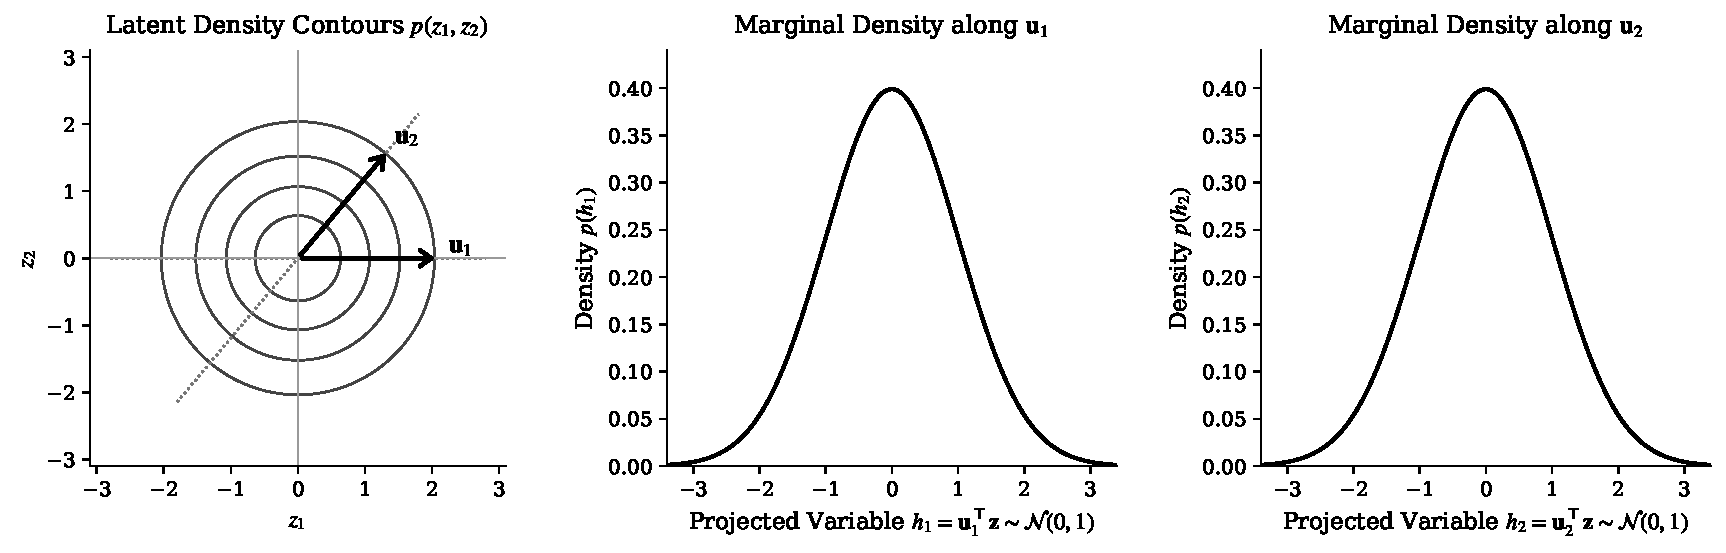
\includegraphics[width=\linewidth]{cramer_wold.pdf}
\caption{Illustration of the Cramér-Wold decomposition. Left: Density contours in latent space $\mathcal{Z}$, showing continuous decomposition along two arbitrary unit directions $\mathbf{u}_1$ and $\mathbf{u}_2$. Center: Marginal density projected along direction $\mathbf{u}_1$. Right: Marginal density projected along direction $\mathbf{u}_2$. The theorem establishes that the joint distribution is uniquely characterized by the complete set of its one-dimensional projections.}
\label{fig:7.1}
\end{figure}

\begin{proposition}[Characterization of the Standard Isotropic Gaussian via Projections]
\label{prop:7.2}
Let $Z \in \mathbb{R}^{d}$ be a random vector. The following statements are equivalent:
\begin{enumerate}[label=(\alph*)]
    \item For every unit direction $u \in \mathbb{S}^{d-1}$, the scalar projection $u^{\top} Z$ follows a standard normal distribution $\mathcal{N}(0, 1)$.
    \item $Z \sim \mathcal{N}(\vec{0}, I_{d})$.
\end{enumerate}
\end{proposition}

\begin{proof}
$(\text{b} \implies \text{a})$. If $Z \sim \mathcal{N}(\vec{0}, I_{d})$, any linear combination $u^{\top} Z$ with $\lVert u \rVert_{2} = 1$ is univariate Gaussian with mean $u^{\top} \vec{0} = 0$ and variance $u^{\top} I_{d} u = \lVert u \rVert_{2}^{2} = 1$. Thus $u^{\top} Z \sim \mathcal{N}(0, 1)$ for all $u \in \mathbb{S}^{d-1}$.

$(\text{a} \implies \text{b})$. Let $W \sim \mathcal{N}(\vec{0}, I_{d})$. By the preceding implication, $u^{\top} W \sim \mathcal{N}(0, 1)$ for all $u \in \mathbb{S}^{d-1}$, matching hypothesis (a) on $Z$. Thus, $Z$ and $W$ have the exact same univariate projection laws along every direction. By the Cram\'er-Wold Theorem (\Cref{thm:7.1}), the joint probability law of a random vector in $\mathbb{R}^{d}$ is uniquely determined by the family of its one-dimensional projections. Therefore $Z \stackrel{d}{=} W$, i.e., $Z \sim \mathcal{N}(\vec{0}, I_{d})$.
\end{proof}

These results shift the paradigm from imposing decorrelation while assuming normality (Jaynes' Bridge) to imposing normality across projections and obtaining statistical independence as an immediate consequence. Moreover, they reduce multivariate normality testing to solving multiple univariate tests in $\mathbb{R}$. All that remains is a univariate normality test that is fully differentiable and compatible with gradient descent.

\section{The Differentiable Epps-Pulley Test}
\label{sec:7.2}

\Cref{prop:7.2} reduces verifying the isotropic normality of $Z \in \mathbb{R}^{d}$ to checking that each univariate projection $u^{\top} Z$ follows a $\mathcal{N}(0, 1)$ distribution. Classical normality tests such as Shapiro-Wilk, Anderson-Darling, or Kolmogorov-Smirnov rely on sample sorting (order statistics) or empirical step cumulative distribution functions, involving non-differentiable comparisons and suprema incompatible with gradient descent.

In 2025, Balestriero and LeCun \cite{balestriero2025lejepa} proposed using the **Epps-Pulley statistic** \cite{epps1983test}, which formulates normality testing in the frequency domain via the characteristic function, achieving smooth differentiability everywhere.

\begin{definition}[Characteristic Function]
\label{def:7.2}
Let $X$ be a real random variable with probability distribution $P_{X}$. The characteristic function of $X$ is the mapping $\phi_{X} \colon \mathbb{R} \to \mathbb{C}$ given by:
\begin{equation}
\label{eq:7.2}
\phi_{X}(t) = \mathbb{E}\left[e^{itX}\right] = \int_{-\infty}^{\infty} e^{itx}\,dP_{X}(x),
\end{equation}
where $i = \sqrt{-1}$ is the imaginary unit.
\end{definition}

The characteristic function exists for any random variable and satisfies L\'evy's Uniqueness Theorem: two random variables have the same probability distribution if and only if they share the exact same characteristic function.

\begin{proposition}[Characteristic Function of $\mathcal{N}(0, 1)$]
\label{prop:7.3}
If $X \sim \mathcal{N}(0, 1)$, its characteristic function is:
\begin{equation}
\label{eq:7.3}
\phi_{0}(t) = e^{-t^{2}/2}.
\end{equation}
\end{proposition}

\begin{proof}
Evaluating the expectation in \Cref{def:7.2}:
\[
\phi_{0}(t) = \int_{-\infty}^{\infty} e^{itx} \frac{1}{\sqrt{2\pi}} e^{-x^{2}/2}\,dx = \frac{1}{\sqrt{2\pi}} \int_{-\infty}^{\infty} \exp\left( -\frac{x^{2} - 2itx}{2} \right) dx.
\]
Completing the square in the exponent, $x^{2} - 2itx = (x - it)^{2} + t^{2}$, yields:
\[
\phi_{0}(t) = e^{-t^{2}/2} \frac{1}{\sqrt{2\pi}} \int_{-\infty}^{\infty} e^{-(x - it)^{2}/2}\,dx = e^{-t^{2}/2},
\]
where the shifted Gaussian contour integral equals $\sqrt{2\pi}$ by Cauchy's Integral Theorem.
\end{proof}

The idea of the Epps-Pulley test is as follows: if $X \sim \mathcal{N}(0, 1)$, its characteristic function $\phi_{X}(t)$ coincides with $\phi_{0}(t) = e^{-t^{2}/2}$ for all $t \in \mathbb{R}$. We can quantify discrepancy via the weighted $L^{2}$ distance between $\phi_{X}$ and $\phi_{0}$:
\begin{equation}
\label{eq:7.4}
T = \int_{-\infty}^{\infty} \left\lvert \phi_{X}(t) - \phi_{0}(t) \right\rvert^{2} w(t)\,dt,
\end{equation}
where $w(t) = \sqrt{\frac{2}{\pi}} e^{-t^{2}}$ is a normalized Gaussian weighting function that concentrates the comparison around low-to-moderate frequencies and allows exact closed-form analytical integration. By the Uniqueness Theorem, $T = 0$ if and only if $X \sim \mathcal{N}(0, 1)$.

In practice, given a finite sample of observations $h_{1}, \dots, h_{n}$ drawn from $X$, we estimate the population characteristic function via the \textbf{Empirical Characteristic Function (ECF)}:
\begin{equation}
\label{eq:7.5}
\hat{\phi}_{n}(t) = \frac{1}{n} \sum_{j=1}^{n} e^{ith_{j}}.
\end{equation}
Substituting $\phi_{X}$ with $\hat{\phi}_{n}$ in the functional (\Cref{eq:7.4}) and evaluating the Gaussian integrals analytically yields the closed-form \textbf{Epps-Pulley statistic} for the sample:
\begin{equation}
\label{eq:7.6}
T(h_{1}, \dots, h_{n}) = 1 + \frac{\sqrt{2}}{n^{2}} \sum_{j=1}^{n} \sum_{k=1}^{n} \exp\left( -\frac{(h_{j} - h_{k})^{2}}{4} \right) - \frac{4}{\sqrt{3}\,n} \sum_{j=1}^{n} \exp\left( -\frac{h_{j}^{2}}{6} \right).
\end{equation}

Crucially, as seen in \Cref{eq:7.6}, the statistic is a smooth sum of radial basis exponential functions; every term is infinitely differentiable ($C^{\infty}$) with respect to the observations $h_{j}$, making it directly usable as a loss function for gradient descent.

\section{The SIGReg Algorithm and the LeWorldModel Loss}
\label{sec:7.3}

\subsection{From Latent Space to Univariate Projections}
\label{sec:7.3.1}

In general representation learning settings (such as video sequences of length $T$ across a batch of size $N$), the encoder $f_{\theta}$ produces a tensor of representations in $\mathbb{R}^{N \times T \times d}$. To apply regularization, this tensor is flattened into a single matrix $Z \in \mathbb{R}^{B \times d}$ with $B = N \cdot T$, gathering all $B$ $d$-dimensional embeddings of the batch. Each row $z_{b} \in \mathbb{R}^{d}$ is the embedding of a specific element.

To evaluate the normality of $Z$ along a unit direction $u \in \mathbb{S}^{d-1}$, we compute the univariate projection of each embedding:
\begin{equation}
\label{eq:7.7}
h_{b} = u^{\top} z_{b}, \qquad b = 1, \dots, B,
\end{equation}
obtaining a vector of $B$ real values $h_{u} = (h_{1}, \dots, h_{B})^{\top} = Z u \in \mathbb{R}^{B}$. Its departure from a standard normal $\mathcal{N}(0, 1)$ is quantified by evaluating the Epps-Pulley statistic $T(h_{u}) = T(h_{1}, \dots, h_{B})$.

\subsection{The SIGReg Regularizer}
\label{sec:7.3.2}

\textbf{SIGReg} (\textit{Sketched-Isotropic-Gaussian Regularizer}) combines the Cram\'er-Wold dimensional reduction with the Epps-Pulley test. At each training step, $M$ unit directions $u^{(1)}, \dots, u^{(M)}$ are sampled uniformly from the unit hypersphere $\mathbb{S}^{d-1}$, the $M$ univariate projections are computed:
\begin{equation}
\label{eq:7.8}
h^{(m)} = Z u^{(m)} \in \mathbb{R}^{B}, \qquad m = 1, \dots, M,
\end{equation}
and the Epps-Pulley statistic is averaged across all $M$ projections:
\begin{equation}
\label{eq:7.9}
\SIGReg(Z) = \frac{1}{M} \sum_{m=1}^{M} T\left(h^{(m)}\right).
\end{equation}

Minimizing this single scalar forces the multivariate distribution of $Z$ to converge toward $\mathcal{N}(\vec{0}, I_{d})$, realizing Barlow's Principle without explicitly computing or regularizing covariance matrices.

The total loss for training \textbf{LeWorldModel} end-to-end is simply:
\begin{equation}
\label{eq:7.10}
\mathcal{L}_{\text{LeWM}} = \mathcal{L}_{\text{pred}} + \lambda \SIGReg(Z),
\end{equation}
with $\mathcal{L}_{\text{pred}} = \frac{1}{N(T - 1)}\sum_{i=1}^{N}\sum_{t=1}^{T-1} \lVert \hat{z}_{t+1}^{(i)} - z_{t+1}^{(i)} \rVert_{2}^{2}$ (\Cref{chap:6}) and $\lambda > 0$ as the sole regularization hyperparameter.

\begin{figure}[H]
\centering
\resizebox{\linewidth}{!}{
\begin{tikzpicture}[
    node distance=1.5cm,
    inputbox/.style={draw, rectangle, rounded corners, minimum width=2.2cm, minimum height=0.8cm, align=center, fill=gray!5, font=\footnotesize\sffamily},
    matbox/.style={draw, rectangle, rounded corners, minimum width=2.5cm, minimum height=1cm, align=center, fill=gray!5, font=\footnotesize\sffamily},
    termbox/.style={draw, rectangle, rounded corners, minimum width=2.5cm, minimum height=1cm, align=center, font=\footnotesize\bfseries},
    arrow/.style={->, >=stealth, thick, rounded corners},
    operator/.style={draw, circle, fill=gray!10, font=\footnotesize\bfseries, inner sep=2pt}
]

\node[inputbox] (z_hat) at (-5.5, 0) {Predictions (Batch)\\$\hat{Z} \in \mathbb{R}^{B \times d}$};
\node[inputbox] (z_tgt) at (-2.0, 0) {Targets (Batch)\\$Z \in \mathbb{R}^{B \times d}$};
\node[inputbox] (z_all) at (5.5, 0) {Representations (Batch)\\$Z \in \mathbb{R}^{B \times d}$};

\node[termbox, fill=red!10] (l_pred) at (-3.75, -2.5) {MSE\\{\scriptsize Mean Squared Error}};
\draw[arrow] (z_hat) |- (l_pred);
\draw[arrow] (z_tgt) |- (l_pred);

\node[draw=blue!30, dashed, rounded corners, fill=blue!2, inner sep=10pt, minimum width=8.5cm, minimum height=4.2cm] (cw_box) at (5.5, -3.2) {};
\node[font=\footnotesize\bfseries, text=blue!80] at (3.8, -1.5) {Cramér-Wold (Projections)};

\node[align=left, font=\scriptsize] (u1) at (2.5, -2.4) {$\mathbf{h}^{(1)} = Z \mathbf{u}^{(1)}$};
\node[font=\scriptsize] at (2.5, -3.2) {$\vdots$};
\node[align=left, font=\scriptsize] (uM) at (2.5, -4.0) {$\mathbf{h}^{(M)} = Z \mathbf{u}^{(M)}$};

\node[inner sep=0pt] at (7.0, -3.2) {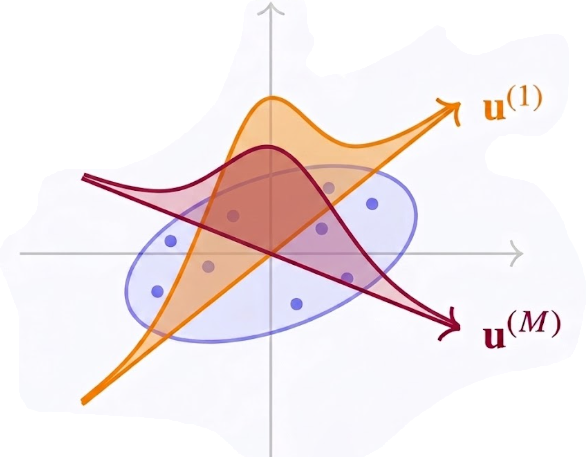
\includegraphics[width=4.5cm]{cramer_wold_new.png}};

\draw[arrow] (z_all) -- (cw_box);

\node[matbox, fill=orange!10, draw=orange!50] (ep1) at (2.5, -6.5) {Epps-Pulley\\$T(\mathbf{h}^{(1)})$};
\node[matbox, fill=purple!10, draw=purple!50] (epM) at (8.5, -6.5) {Epps-Pulley\\$T(\mathbf{h}^{(M)})$};
\node[font=\footnotesize\bfseries] (dots) at (5.5, -6.5) {$\dots$};

\draw[arrow, orange] (2.5, -5.3) -- (ep1.north);
\draw[arrow, purple] (8.5, -5.3) -- (epM.north);

\node[operator] (avg) at (5.5, -8) {$\frac{1}{M} \sum$};
\draw[arrow, orange] (ep1.south) |- (avg.west);
\draw[arrow, purple] (epM.south) |- (avg.east);

\node[termbox, fill=blue!10] (l_sigreg) at (5.5, -9.5) {$\SIGReg(Z)$\\{\scriptsize Normality}};
\draw[arrow] (avg) -- (l_sigreg);

\node[operator] (plus) at (0.9, -11) {$+$};
\draw[arrow] (l_pred.south) |- (plus.west);
\draw[arrow] (l_sigreg.south) |- (plus.east);
\node[anchor=south west, font=\footnotesize] at (plus.east) {$\times \lambda$};

\node[termbox, fill=green!15, minimum width=4cm] (l_total) at (0.9, -12.5) {$\mathcal{L}_{\text{LeWM}}$\\{\scriptsize $\mathcal{L}_{\text{pred}} + \lambda \SIGReg(Z)$}};
\draw[arrow] (plus) -- (l_total);

\begin{scope}[on background layer]
    \node[draw=gray, dashed, rounded corners, fit=(l_pred)(z_hat)(z_tgt), inner sep=12pt, fill=gray!3] (pred_bg) {};
    \node[anchor=south, font=\footnotesize\bfseries, text=gray!60] at (pred_bg.north) {$\mathcal{L}_{\text{pred}}$};
    \node[draw=blue!40, dashed, rounded corners, fit=(cw_box)(ep1)(epM)(avg)(l_sigreg), inner sep=12pt, fill=blue!1] (sigreg_bg) {};
    \node[anchor=south, font=\footnotesize\bfseries, text=blue!70] at (sigreg_bg.north) {$\SIGReg(Z)$};
\end{scope}

\end{tikzpicture}
}
\caption{Detailed diagram of the LeWorldModel loss function. Left: The prediction branch optimizes similarity in latent space via MSE. Right: The regularization branch applies SIGReg to batch representations $Z \in \mathbb{R}^{B \times d}$: via Cram\'er-Wold, multivariate data are projected onto $M$ random unit directions $\mathbf{u}^{(m)}$, univariate normality is evaluated with the Epps-Pulley statistic $T$ on each projection, and results are averaged. Both terms are combined weighted by $\lambda$.}
\label{fig:7.2}
\end{figure}

\begin{figure}[H]
\centering
\resizebox{\linewidth}{!}{
\begin{tikzpicture}[
    node distance=1.5cm,
    obsbox/.style={draw=gray!50, rectangle, rounded corners, minimum width=2cm, minimum height=1cm, align=center, fill=gray!5, font=\footnotesize\sffamily},
    encbox/.style={draw=blue!40, rectangle, rounded corners, minimum width=2cm, minimum height=1cm, align=center, fill=blue!5, font=\footnotesize\sffamily},
    predbox/.style={draw=violet!40, rectangle, rounded corners, minimum width=2.2cm, minimum height=1cm, align=center, fill=violet!5, font=\footnotesize\sffamily},
    lossbox/.style={draw=red!40, rectangle, rounded corners, minimum width=2.5cm, minimum height=1.2cm, align=center, fill=red!10, font=\footnotesize\bfseries},
    arrow/.style={->, >=stealth, thick, rounded corners},
    state/.style={font=\footnotesize\sffamily, align=center}
]

    \node[obsbox] (ot) at (0, 0) {Observation\\$o_t$};
    \node[encbox] (enc_t) at (2.8, 0) {Encoder\\$f_\theta$};
    \node[state] (zt) at (5.0, 0) {State\\$z_t$};
    \node[predbox] (pred) at (7.8, 0) {Predictor\\$g_\phi$};
    \node[state] (zhat) at (10.4, 0) {Prediction\\$\hat{z}_{t+1}$};

    \node[obsbox] (ot1) at (0, -2.2) {Observation\\$o_{t+1}$};
    \node[encbox] (enc_t1) at (2.8, -2.2) {Encoder\\$f_\theta$};
    \node[state] (zt1) at (10.4, -2.2) {Target\\$z_{t+1}$};

    \draw[arrow] (ot) -- (enc_t);
    \draw[arrow] (enc_t) -- (zt);
    \draw[arrow] (zt) -- (pred);
    \draw[arrow] (pred) -- (zhat);

    \draw[arrow] (ot1) -- (enc_t1);
    \draw[arrow] (enc_t1) -- (zt1);

    \node[lossbox] (loss_asym) at (13.5, -1.1) {$\mathcal{L}_{\text{LeWM}}$};
    \draw[arrow] (zhat.east) to[out=0, in=180] (loss_asym.west);
    \draw[arrow] (zt1.east) to[out=0, in=180] (loss_asym.west);

    \draw[<->, dashed, thick, gray!70] (enc_t.south) -- node[right, font=\scriptsize, text=gray!80] {shared weights} (enc_t1.north);

    \begin{scope}[on background layer]
        \node[draw=orange!30, dashed, rounded corners=8pt, fit=(zt) (zhat) (pred), inner sep=10pt, fill=orange!3] (pred_zone) {};
        \node[anchor=south, font=\scriptsize\bfseries, text=orange!80] at (pred_zone.north) {Latent dynamics};
    \end{scope}

\end{tikzpicture}
}
\caption{Base Joint Embedding Predictive Architecture (JEPA) used in LeWorldModel. An encoder $f_\theta$ (with shared weights, requiring no EMA or stop-gradient) extracts abstract representations from observations, while a predictor $g_\phi$ simulates the dynamic transition in latent space anticipating $\hat{z}_{t+1}$ from current state $z_t$.}
\label{fig:7.3}
\end{figure}

\section{Closing Barlow's Circle}
\label{sec:7.4}

This chapter culminates the evolutionary journey of representation learning within the Joint Embedding paradigm, resolving the primary theoretical limitation of the non-contrastive methods analyzed in \Cref{chap:5}.

Barlow's redundancy reduction principle \cite{barlow1961possible} demands mutual statistical independence among latent variables. Under the classical frameworks of Barlow Twins and VICReg, this condition was approximated by zeroing linear covariances (second-order moments)---a simplification that Jaynes' Bridge declares exact only under a multivariate normality hypothesis that those methods never actively guaranteed.

Through the SIGReg regularizer, this theoretical gap is definitively closed:
\begin{itemize}
    \item \textbf{Grounded in Cram\'er-Wold:} Projects the high-dimensional latent space onto multiple random one-dimensional directions, reducing an intractable multivariate problem to a parallel family of univariate evaluations.
    \item \textbf{Differentiability via Epps-Pulley:} Evaluates the normality of each projection in the space of characteristic functions analytically and with full differentiability, smoothly driving the latent distribution toward an isotropic Gaussian $\mathcal{N}(\vec{0}, I_{d})$.
\end{itemize}

By actively enforcing spherical normality of the representations, linear decorrelation and full statistical independence become strictly equivalent. In this way, SIGReg not only simplifies computational complexity and eliminates the conflicting gradients of PLDM/VICReg, but realizes Barlow's principle in its original mathematical purity.


\begin{figure}[H]
\centering
\resizebox{\linewidth}{!}{%
\begin{tikzpicture}[
    node distance=0.5cm,
    problem/.style={draw=red!70!black, rounded corners, minimum width=2cm, minimum height=1.2cm, align=center, fill=red!8, font=\scriptsize, text=black},
    solution/.style={draw=blue!70!black, rounded corners, minimum width=2cm, minimum height=1.2cm, align=center, fill=blue!8, font=\scriptsize, text=black},
    assumption/.style={draw=yellow!70!black, rounded corners, minimum width=2cm, minimum height=1.2cm, align=center, fill=yellow!10, font=\scriptsize, text=black},
    final/.style={draw=green!60!black, rounded corners, minimum width=2cm, minimum height=1.2cm, align=center, fill=green!10, font=\scriptsize, thick, text=black},
    arrow/.style={->, >=stealth, thick, gray!70},
    label/.style={font=\tiny, text=black, align=center}
]

\node[problem] (collapse) {Trivial and\\Dimensional\\Collapse};
\node[label, above=0.1cm of collapse] {Chap.~3\\(1993)};

\node[solution, right=of collapse] (contrastive) {Contrastive\\Losses\\$\mathcal{L}_{\text{neg}}$};
\node[label, above=0.1cm of contrastive] {Chap.~4\\(2006)};

\node[problem, right=of contrastive] (exp) {Exponential\\Scaling\\$\mathcal{O}(e^d)$};

\node[solution, right=of exp] (barlow) {Barlow Twins\\VICReg\\(decorrelation)};
\node[label, above=0.1cm of barlow] {Chap.~5\\(2021--2022)};

\node[assumption, right=of barlow] (gauss) {Unverified\\Gaussian\\Hypothesis};

\node[solution, right=of gauss] (jepa) {V-JEPA\\(ad-hoc\\heuristics)};
\node[label, above=0.1cm of jepa] {Chap.~6\\(2022--2025)};

\node[final, right=of jepa] (sigreg) {\textbf{SIGReg}\\Enforced\\Normality};
\node[label, above=0.1cm of sigreg] {Chap.~7\\(2025--2026)};

\draw[arrow] (collapse) -- (contrastive);
\draw[arrow] (contrastive) -- (exp);
\draw[arrow] (exp) -- (barlow);
\draw[arrow] (barlow) -- (gauss);
\draw[arrow] (gauss) -- (jepa);
\draw[arrow] (jepa) -- (sigreg);

\draw[->, >=stealth, thick, green!50!black, dashed] (sigreg.south) to[out=-90, in=-90, looseness=0.5] node[below, font=\scriptsize\itshape, text=green!50!black, yshift=-0.1cm] {Closing Barlow's Principle} (barlow.south);

\node[below=1.8cm of collapse, font=\scriptsize, anchor=west] (leg) {
    {\tikz\draw[fill=red!8, draw=red!70!black, rounded corners] (0,0) rectangle (0.4,0.25);} Problem \quad
    {\tikz\draw[fill=blue!8, draw=blue!70!black, rounded corners] (0,0) rectangle (0.4,0.25);} Solution \quad
    {\tikz\draw[fill=yellow!10, draw=yellow!70!black, rounded corners] (0,0) rectangle (0.4,0.25);} Pending hypothesis \quad
    {\tikz\draw[fill=green!10, draw=green!60!black, rounded corners] (0,0) rectangle (0.4,0.25);} Final resolution
};

\end{tikzpicture}%
}
\caption{Evolutionary narrative arc of Chapters~\ref{chap:3}--\ref{chap:7}. Each limitation (red) motivates the subsequent solution (blue). The Gaussian hypothesis (yellow), implicitly assumed by Barlow Twins and VICReg but never verified, is finally explicitly enforced by SIGReg (green), closing Barlow's principle in its original mathematical purity.}
\label{fig:7.4}
\end{figure}


\section{Limitations of the SIGReg / LeWorldModel Framework}
\label{sec:7.5}

\subsection{Theoretical and Practical Limitations}
\label{sec:7.5.1}

Although the framework developed in this chapter resolves the tension raised in \Cref{sec:6.5}, it is not free of assumptions that merit examination with the same rigor applied to PLDM and V-JEPA.

The first limitation concerns the choice of target distribution. SIGReg enforces isotropic Gaussianity on $\mathcal{Z}$ because it is the unique distribution under which Jaynes' Bridge guarantees the equivalence between zero covariance and statistical independence. This raises a natural question: is Gaussianity merely a convenient technical device to ensure statistical independence, or is it also the right distribution for recovering the true underlying latent variables of the environment? This question was recently addressed by Klindt, LeCun, and Balestriero \cite{klindt2026when}, who formally proved that, under dynamics with additive Gaussian noise, the Gaussian distribution is indeed the unique latent distribution allowing the model to linearly recover the true latent state variables of the system. Conversely, if the true underlying dynamics of the environment are strongly non-Gaussian (e.g., discrete topological transitions or heavy-tailed shocks), enforcing an isotropic Gaussian prior on $\mathcal{Z}$ loses this identifiability guarantee, suggesting that modeling non-Gaussian worlds will require architectural adaptations beyond hyperparameter tuning \cite{klindt2026when}.

The second limitation is computational. The differentiable Epps-Pulley test introduced in \Cref{sec:7.2} evaluates normality via $M$ random one-dimensional projections, relying on the Cram\'er-Wold Theorem (\Cref{sec:7.1}, \Cref{thm:7.1}). The number of random projections $M$ required for this sketched approximation to faithfully constrain all directions of $\mathbb{R}^{d}$ grows with the dimension of $\mathcal{Z}$, and the pairwise kernel sum in \Cref{eq:7.6} scales quadratically as $\mathcal{O}(B^{2})$ in the batch size $B$.

% =========================================================================
% CHAPTER 8
% =========================================================================
\chapter{Conclusions and Future Directions}
\label{chap:8}

\section{The Guiding Thread: From Collapse to Its Resolution}
\label{sec:8.1}

\Cref{chap:1} posed as the guiding thread of this thesis the resolution of the most persistent obstacle in the Joint Embedding paradigm: \textit{representation collapse}, wherein the network minimizes energy to zero by mapping all inputs to a trivial constant $f_{\theta}(x) = c$. Each chapter addressed a distinct stage of this problem:

\begin{itemize}
    \item \textbf{\Cref{chap:2}} introduced EBMs as a unifying framework for compatibility learning and established, through Jaynes' Principle of Maximum Entropy, the physical basis for probability assignments over $\mathcal{Z}$. That same principle reappears in concrete form in \Cref{chap:7}: the isotropic Gaussian distribution $\mathcal{N}(\vec{0}, I_{d})$ that SIGReg enforces over $\mathcal{Z}$ is precisely the maximum entropy distribution under fixed unit variance.
    \item \textbf{\Cref{chap:3}} analytically proved the vulnerability of Siamese networks to both constant and dimensional collapse when trained solely with positive alignment ($\mathcal{L}_{\text{pos}}$), showing via spectral gradient flow that $\mathcal{L}_{\text{pos}}$ acts as a contraction operator.
    \item \textbf{\Cref{chap:4}} showed that contrastive learning prevents collapse via repulsive forces generated by negative samples, at the cost of an exponential sample complexity $\mathcal{O}((1/\epsilon)^{d})$ dictated by the covering number of the hypersphere $\mathbb{S}^{d-1}$.
    \item \textbf{\Cref{chap:5}} examined the non-contrastive revolution inspired by Barlow's hypothesis, demonstrating that Barlow Twins and VICReg avoid collapse via second-order matrix regularizations, but rely on Jaynes' Bridge---whose guarantee of statistical independence holds only under an unverified normality assumption on $\mathcal{Z}$.
    \item \textbf{\Cref{chap:6}} extended the framework to temporal World Models and JEPAs, showing that PLDM inherits this unverified Gaussian dependence alongside severe gradient interference across its seven loss terms, whereas V-JEPA avoids collapse via dynamic architectural heuristics (EMA and stop-gradient) lacking a unified statistical foundation.
    \item \textbf{\Cref{chap:7}} presented LeWorldModel and its isotropic probabilistic regularizer, SIGReg, which combines the Cram\'er-Wold Theorem and the differentiable Epps-Pulley characteristic-function test to actively enforce multivariate normality, closing Barlow's circle rigorously and without heuristics.
\end{itemize}

\section{Future Directions}
\label{sec:8.2}

While this thesis establishes the theoretical foundations of Joint Embedding World Models, their practical deployment is only beginning to unfold. The limitations analyzed throughout this work point toward two major avenues for future research, aligned with the contemporary vision of \textbf{H-JEPA} (Hierarchical JEPA) and its extension to complex dynamical systems:

\begin{enumerate}
    \item \textbf{Transition to Hierarchical World Models (H-JEPA):} Current Vision-Language-Action (VLA) models in robotics rely heavily on behavioral cloning and lack explicit planning capabilities because they do not possess an internal predictive model of the consequences of their actions. While action-conditioned JEPAs enable latent-space planning, flat predictive architectures such as LeWorldModel remain unstable over long planning horizons \cite{klindt2026when}. A promising direction is hierarchical prediction: structuring the latent space across multiple levels of temporal and spatial abstraction. In H-JEPA, lower levels perform short-term predictions retaining fine-grained detail for millisecond motor control, while higher levels operate over extended temporal horizons, generating abstract subgoals for lower-level planners. Integrating rigorous probabilistic regularizers like SIGReg across multiple hierarchical levels without inducing inter-level collapse remains a central open problem.
    \item \textbf{Application to Complex Dynamical Systems:} Classical optimal control requires system dynamics to be described by a small set of explicit differential equations. JEPA-based World Models open the door to learning latent simulators purely from observational data in domains where analytical modeling is intractable---ranging from aerodynamic turbulence prediction in jet engines and chemical plant control to materials design, macroeconomic dynamics, and personalized clinical treatment planning.
\end{enumerate}

Both lines ultimately converge on a single foundational challenge: endowing the representation space with a statistical geometry that is simultaneously rich and stable, capable of sustaining multi-step prediction without collapsing under its own weight. If differential calculus provided the language to describe the continuous systems of classical physics, the statistical geometry of latent spaces may well be called upon to play an analogous role for machines that, in the coming decades, will learn to anticipate the future before acting upon it.

% =========================================================================
% APPENDICES
% =========================================================================
\appendix

\chapter{Foundations of Deep Learning}
\label{app:A}

This appendix summarizes the fundamental deep learning concepts that serve as the technical basis for the developments in the main text. For comprehensive treatments, we refer the reader to Goodfellow et al.\ \cite{goodfellow2016deep}, the foundational work on backpropagation by Rumelhart et al.\ \cite{rumelhart1986learning}, and the review on representation learning by Bengio et al.\ \cite{bengio2013representation}.

\section{The Multilayer Perceptron (MLP)}
\label{sec:A.1}

The fundamental building block of the architectures studied in this work is the feedforward neural network or \textbf{Multilayer Perceptron (MLP)} \cite{goodfellow2016deep}. An $L$-layer MLP defines a parameterized mapping $f_{\theta} \colon \mathbb{R}^{d_{0}} \to \mathbb{R}^{d_{L}}$ through the composition of affine transformations and elementwise nonlinearities.

\begin{definition}[Feedforward Neural Network]
\label{def:A.1}
Let $d_{0}, d_{1}, \dots, d_{L} \in \mathbb{N}$ be the sequence of layer dimensions. For each layer $l = 1, \dots, L$, define a weight matrix $W^{(l)} \in \mathbb{R}^{d_{l} \times d_{l-1}}$ and a bias vector $b^{(l)} \in \mathbb{R}^{d_{l}}$. Denoting the pre-activation vector at layer $l$ by $z^{(l)} = W^{(l)} h^{(l-1)} + b^{(l)}$, the forward pass is defined recursively as:
\begin{equation}
\label{eq:A.1}
h^{(0)} = x, \qquad h^{(l)} = \sigma\left(W^{(l)} h^{(l-1)} + b^{(l)}\right), \; l = 1, \dots, L-1, \qquad f_{\theta}(x) = W^{(L)} h^{(L-1)} + b^{(L)},
\end{equation}
where $\sigma \colon \mathbb{R} \to \mathbb{R}$ is a nonlinear activation function applied componentwise. The set of trainable parameters is $\theta = \{W^{(l)}, b^{(l)}\}_{l=1}^{L}$.
\end{definition}

Common activation functions include:
\begin{itemize}
    \item \textbf{ReLU (Rectified Linear Unit):} $\sigma(z) = \max(0, z)$. The default choice in modern architectures due to its computational efficiency and mitigation of vanishing gradients in the positive regime.
    \item \textbf{Sigmoid:} $\sigma(z) = (1 + e^{-z})^{-1} \in (0, 1)$. Historically used in output layers for binary classification.
    \item \textbf{GELU (Gaussian Error Linear Unit):} $\sigma(z) = z \cdot \Phi(z)$, where $\Phi$ is the standard normal cumulative distribution function. Widely used in Transformers.
\end{itemize}

\subsection{Final Projection Layer and Pre-Activation Features}
\label{sec:A.1.1}

In theoretical analyses of deep learning architectures (such as our study of dimensional collapse in \Cref{sec:3.3}), it is standard practice to abstract the nonlinear complexity of the first $L-1$ layers into a feature extractor mapping the input $x$ to a feature vector $\phi(x) \in \mathbb{R}^{m}$, followed by a purely linear final projection layer parameterized by $W \in \mathbb{R}^{d \times m}$ (omitting the bias without loss of generality for centered features):
\begin{equation}
\label{eq:A.2}
f_{W}(x) = W \phi(x).
\end{equation}

\section{Loss Functions}
\label{sec:A.2}

\subsection{Mean Squared Error (MSE)}
\label{sec:A.2.1}

In regression and continuous prediction tasks, the least-squares loss over a dataset $\{(x_{i}, y_{i})\}_{i=1}^{N}$ is defined as:
\begin{equation}
\label{eq:A.3}
\mathcal{L}_{\text{MSE}}(\theta) = \frac{1}{N} \sum_{i=1}^{N} \lVert f_{\theta}(x_{i}) - y_{i} \rVert_{2}^{2}.
\end{equation}
Under multimodal uncertainty in pixel space, minimizing \Cref{eq:A.3} forces the model to predict the conditional expectation $\mathbb{E}[y \mid x]$, which averages over plausible futures and produces visual blurriness.

\subsection{Cross-Entropy}
\label{sec:A.2.2}

For classification tasks with $C$ classes, the cross-entropy loss measures the Kullback-Leibler divergence between the true one-hot distribution $y_{i}$ and the predicted categorical distribution $q_{\theta}(\cdot \mid x_{i})$:
\begin{equation}
\label{eq:A.4}
\mathcal{L}_{\text{CE}}(\theta) = -\frac{1}{N} \sum_{i=1}^{N} \sum_{c=1}^{C} y_{ic} \log q_{\theta}(c \mid x_{i}),
\end{equation}
where $q_{\theta}(c \mid x_{i}) = \softmax(f_{\theta}(x_{i}))_{c}$. This is the discrete analogue of the negative log-likelihood under the Boltzmann-Gibbs distribution (\Cref{eq:2.3}).

\subsection{Minibatch Approximation}
\label{sec:A.2.3}

Given a subsample (minibatch) $\mathcal{B} = \{x_{i}\}_{i=1}^{B} \subset \mathcal{X}$ of size $B \ll N$ drawn uniformly from the training distribution, the population expectation of the loss is approximated by the empirical average:
\begin{equation}
\label{eq:A.5}
\mathbb{E}_{x \sim p(x)}[\mathcal{L}(x)] \approx \frac{1}{B} \sum_{i=1}^{B} \mathcal{L}(x_{i}).
\end{equation}

\section{Error Backpropagation}
\label{sec:A.3}

\subsection{The Chain Rule on Computational Graphs}
\label{sec:A.3.1}

Backpropagation \cite{rumelhart1986learning} is the systematic application of the multivariable chain rule to the compositional structure of an MLP. Defining the pre-activation vector at layer $l$ as $z^{(l)} = W^{(l)} h^{(l-1)} + b^{(l)}$ and the local error sensitivity with respect to pre-activations as $\delta^{(l)} = \nabla_{z^{(l)}} \mathcal{L} \in \mathbb{R}^{d_{l}}$, the gradient with respect to the weight matrix $W^{(l)} \in \mathbb{R}^{d_{l} \times d_{l-1}}$ is given by the outer product:
\begin{equation}
\label{eq:A.6}
\frac{\partial \mathcal{L}}{\partial W^{(l)}} = \frac{\partial \mathcal{L}}{\partial z^{(l)}} \frac{\partial z^{(l)}}{\partial W^{(l)}} = \delta^{(l)} \left(h^{(l-1)}\right)^{\top},
\end{equation}
where $\delta^{(l)}$ is computed recursively backward from the output layer $L$:
\begin{equation}
\label{eq:A.7}
\delta^{(L)} = \nabla_{z^{(L)}} \mathcal{L}, \qquad \delta^{(l)} = \left( (W^{(l+1)})^{\top} \delta^{(l+1)} \right) \odot \sigma'\left(W^{(l)} h^{(l-1)} + b^{(l)}\right),
\end{equation}
with $\odot$ denoting the elementwise Hadamard product and $\sigma'$ the derivative of the activation function.

\subsection{Stochastic Gradient Descent (SGD) and Adam}
\label{sec:A.3.2}

Once gradients are computed via \Cref{eq:A.6,eq:A.7}, parameters are updated iteratively. The Stochastic Gradient Descent (SGD) update rule is:
\begin{equation}
\label{eq:A.8}
\theta_{t+1} = \theta_{t} - \eta \nabla_{\theta} \mathcal{L}_{\mathcal{B}_{t}}(\theta_{t}),
\end{equation}
where $\eta > 0$ is the learning rate and $\mathcal{L}_{\mathcal{B}_{t}}$ is the loss evaluated on minibatch $\mathcal{B}_{t}$. In practice, the \textbf{Adam} optimizer \cite{goodfellow2016deep} maintains exponential moving averages of the first and second moments of the gradient to adapt the learning rate per parameter.

% =========================================================================
% APPENDIX B
% =========================================================================
\chapter{Notions of Linear Algebra}
\label{app:B}

This appendix compiles the core linear algebra concepts used throughout this thesis to analyze dimensional collapse and learning dynamics in Siamese architectures.

\section{Covariance Matrix, Rank, and Kernel}
\label{sec:B.1}

Let $Z = f_{W}(X) \in \mathbb{R}^{d}$ be a random vector with mean vector $\mu = \mathbb{E}[Z]$. Its population covariance matrix is defined as:
\begin{equation}
\label{eq:B.1}
\Sigma_{\mathcal{Z}} = \mathbb{E}\left[ (Z - \mu)(Z - \mu)^{\top} \right] \in \mathbb{R}^{d \times d}.
\end{equation}
By construction, $\Sigma_{\mathcal{Z}}$ is symmetric ($\Sigma_{\mathcal{Z}} = \Sigma_{\mathcal{Z}}^{\top}$) and positive semidefinite ($v^{\top} \Sigma_{\mathcal{Z}} v \geq 0$ for all $v \in \mathbb{R}^{d}$). The quadratic form $v^{\top} \Sigma_{\mathcal{Z}} v$ equals the variance of the scalar projection of $Z$ onto the direction $v$:
\begin{equation}
\label{eq:B.2}
\Var(v^{\top} Z) = v^{\top} \Sigma_{\mathcal{Z}} v.
\end{equation}

The \textbf{kernel} (or null space) of $\Sigma_{\mathcal{Z}}$, denoted $\Ker(\Sigma_{\mathcal{Z}})$, is the vector subspace of $\mathbb{R}^{d}$ comprising all directions along which the representation has zero variance:
\begin{equation}
\label{eq:B.3}
\Ker(\Sigma_{\mathcal{Z}}) = \left\{ v \in \mathbb{R}^{d} \;\middle|\; \Sigma_{\mathcal{Z}} v = \vec{0} \right\}.
\end{equation}
By the \textbf{Rank-Nullity Theorem}, for any $d \times d$ matrix:
\begin{equation}
\label{eq:B.4}
d = \rank(\Sigma_{\mathcal{Z}}) + \dim(\Ker(\Sigma_{\mathcal{Z}})).
\end{equation}
Thus, rank deficiency ($\rank(\Sigma_{\mathcal{Z}}) = r < d$) inevitably implies the existence of a non-trivial null subspace of dimension $d - r$, corresponding to dimensional collapse (\Cref{sec:3.3}).

\section{Spectral Theorem for Symmetric Matrices}
\label{sec:B.2}

\begin{theorem}[Spectral Theorem]
\label{thm:B.1}
Every real symmetric matrix $A \in \mathbb{R}^{d \times d}$ is orthogonally diagonalizable. That is, there exist an orthogonal matrix $Q \in \mathbb{R}^{d \times d}$ ($Q^{\top} Q = Q Q^{\top} = I_{d}$) and a real diagonal matrix $\Lambda = \diag(\lambda_{1}, \dots, \lambda_{d})$ such that:
\begin{equation}
\label{eq:B.5}
A = Q \Lambda Q^{\top},
\end{equation}
where the columns of $Q$ form an orthonormal basis of eigenvectors of $A$, and the diagonal entries of $\Lambda$ are the corresponding real eigenvalues $\lambda_{i} \in \mathbb{R}$.
\end{theorem}

If $A$ is also positive semidefinite (as is any covariance matrix $\Sigma_{\mathcal{Z}}$), all its eigenvalues are non-negative ($\lambda_{i} \geq 0$), and $\rank(A)$ equals the number of strictly positive eigenvalues.

\section{Gradient Flow and Spectral Decoupling}
\label{sec:B.3}

In discrete-time gradient descent with learning rate $\eta > 0$ and loss $\mathcal{L}(W)$, the weight update rule is:
\begin{equation}
\label{eq:B.6}
W_{t+1} = W_{t} - \eta \nabla_{W} \mathcal{L}(W_{t}),
\end{equation}
which can be rearranged as a finite-difference quotient:
\begin{equation}
\label{eq:B.7}
\frac{W_{t+1} - W_{t}}{\eta} = -\nabla_{W} \mathcal{L}(W_{t}).
\end{equation}
Taking the infinitesimal step limit ($\eta \to 0$) yields the continuous-time ordinary differential equation (ODE) known as \textbf{Gradient Flow}:
\begin{equation}
\label{eq:B.8}
\dot{W}(t) = -\nabla_{W} \mathcal{L}(W(t)).
\end{equation}

When the loss gradient is linear in $W$, such as $\nabla_{W} \mathcal{L}(W) = W \Sigma$ for a symmetric positive semidefinite matrix $\Sigma = Q \Lambda Q^{\top}$, introducing the orthogonal change of variables $\tilde{W}(t) = W(t) Q$ transforms the coupled matrix ODE $\dot{W}(t) = -W(t) \Sigma$ into the completely decoupled diagonal system:
\begin{equation}
\label{eq:B.9}
\dot{\tilde{W}}(t) = -\tilde{W}(t) \Lambda.
\end{equation}
For each scalar entry $\tilde{w}_{ij}(t)$, the resulting equation is $\dot{\tilde{w}}_{ij}(t) = -\lambda_{j} \tilde{w}_{ij}(t)$, whose exact analytical solution is:
\begin{equation}
\label{eq:B.10}
\tilde{w}_{ij}(t) = \tilde{w}_{ij}(0) e^{-\lambda_{j} t}.
\end{equation}
This closed-form solution reveals that the rate of contraction along each principal axis is governed exclusively by the spectrum of $\Sigma$: large eigenvalues ($\lambda_{j} \gg 0$) drive rapid exponential decay toward the origin, whereas null-space directions ($\lambda_{j} = 0$) remain invariant (\Cref{sec:3.3}).

% =========================================================================
% BIBLIOGRAPHY
% =========================================================================

\backmatter

\bibliographystyle{acm}
\bibliography{referencias}

\end{document}
